% arara: xelatex: { shell: true, interaction: nonstopmode } if changed('tex') || changed(toFile('fefudoc.cls'))
%arara: biber if changed('bib') || changed('bcf') || changed('bbl')
%arara: xelatex: { synctex: true, shell: true } if changed('aux')
% !TeX document-id = {2e2f2d46-ef9b-47ad-990b-8fdc6dcf34fb}
% !TeX program = xelatex
% !TeX encoding = UTF-8
% !TeX spellcheck = ru_RU
% !TeX TXS-program:compile=txs:///xelatex/[--shell-escape]|txs:///view-pdf
% !TeX TXS-program:bibliography = txs:///biber

% Тип документа:
\documentclass[report, draught]{fefudoc}

% Используемые этим документом расширения языка Latex:
\usepackage{enumitem} %кастомизация списков (см. раздел "Списки")
% математика (см. раздел "формулы")
\usepackage{mathtools} %основные математикие операторы и шрифты
\usepackage{amsfonts} %доп. математические шрифты
\usepackage{amssymb, mathabx} %доп. математические символы
%Таблицы (см. раздел "Таблицы")
\usepackage{tabularx} %таблицы заданной ширины с ячейками с длинным текстом и автоматическим переносом строк
\usepackage{multirow} % объединение нескольких строк таблиц в одну
\usepackage{threeparttable} % выравнивание заголовков таблиц
\usepackage{longtable} %длинные таблицы в несколько страниц
\usepackage{makecell} %доп. форматирование ячеек таблиц
\renewcommand\theadfont{\normalsize\bfseries} %сделать заголовки таблиц из makecell нормального размера и выделить их жирным
\usepackage{hhline} % двойные горизонтальные линии в таблицах
%Рисунки, см. раздел "Рисунки"
\usepackage{graphicx} %вставка рисунков из файлов
\usepackage[font=normalsize]{subfig} %составные рисунки с подрисунками
\usepackage{tikz} %рисование в LaTeX с помощью TikZ (см. раздел "Рисование непосредственно в LaTeX")
%Заметки на полях документа (см. раздел "Заметки на полях")
\usepackage{marginnote}
\usetikzlibrary{shapes, arrows.meta, positioning, calc, datavisualization, datavisualization.formats.functions, , datavisualization.polar} %расширения TikZ
%Алгоритмы и исходный код (см. раздел "Алгоритмы и исходный код")
\usepackage[boxed]{algorithm2e}
\usepackage{pgf-umlsd}
\usepackage{listings}
\lstset{ %общие параметры расширения listings
	basicstyle=\ttfamily\small,
	keywordstyle=\bfseries,
	commentstyle=\itshape,
	keepspaces=true,
	showstringspaces=false,
	columns=flexible,
	inputencoding=utf-8,
	extendedchars=true,
	frame=single,
	tabsize=2,
	texcl=true
}
%Список литературы.
\usepackage{biblatex}
\addbibresource{example-sources.bib} %Файл со списком литературы.

\location{Владивосток}
\Institute{Политехнический институт (Школа)}
\Department{Департамент электроники, телекоммуникации и приборостроения}
\specialty{11.03.02} %коды специальностей приведены в Общероссийском классификаторе 009-2016,
                     % а также в файлах details/barchelorspecialties.def (бакалавры)
					 % и в details/masterspecialties.def (магистранты)
\profile{Системы радиосвязи и радиодоступа}
\discipline{Параллельное программирование}

%Автор:
\author{Б3121-11.03.02втц}{Сидоров Иван Петрович}
%Преподаватель:
\teacher{кандидат технических наук}{}{доцент департамента ЭТиП}{Чусов Андрей Александрович}

%Название работы
\title{Использование \LaTeX{} для написания рефератов} %Название

\year=2023

\begin{document}
\frontpage
\tableofcontents

\section*{Введение}
Система верстки текстов \LaTeX{} \cite{Lamport96} предназначена для автоматизации оформления текстовых документов согласно требованиям, которые предоставляются выпускающей организацией (например, издательством журнала или книг, университетом и~т.~п.) в виде правил на формальном языке (обычно хранящихся в текстовых файлах с расширением ".CLS").

Главным преимуществом \LaTeX{} по сравнению с WYSIWYG-редакторами ("What You See Is What You Get"), такими как Microsoft Word, является возможность абстрагировать автора набираемого текста от специфических правил оформления, налагаемых той или иной организацией, и дать возможность автору сосредоточить свои усилия на сути, которую он хочет передать, а не на оформлении.
Кроме этого, программное обеспечение языка \LaTeX{} является свободным, то есть не принадлежащим кому-либо, а значит несанкционируемым и бесплатным.

Ценой этого удобства является необходимость в некоторой степени освоить вероятно непривычный язык \LaTeX{} и, возможно, более фундаментальный  и нижележащий язык \TeX{} \cite{TheTexBook}.

Поскольку система верстки \LaTeX{} была создана в США, в России она распространена слабо, в основном на западе страны, в ВУЗах вроде МГУ и МФТИ \cite{ctan-disser-mipt}, а также в РАН \cite{RAS-latex}, вследствие существовавших долгое время проблем с шрифтами и специфическими правилами русского языка.
Вместе с тем, инструменты, реализующие язык \LaTeX{}, развиваются, и с их помощью сегодня уже можно создавать документы, удовлетворяющие общепринятым в России требованиям (за исключением, конечно, случаев когда то или иное издательство специально требует формата DOC).

Настоящий набор документов предоставляет набор правил для оформления документов в соответствии с нормативами ДВФУ.
Этот набор включает в себя правила для различных типов документов, часть которых еще не закончена.
Примеры оформления приведены в различных файлах с расширением "TEX" корневой директории, эти примеры не требуются для функционирования системы, и лишние, не нужные, файлы можно удалить, чтобы они не мешались.
Вместе с тем, эти примеры удобно модифицировать под собственные нужды, заменяя их содержание.

Настоящий файл является примером реферата.
В качестве содержимого, в нем описаны основные, наиболее часто необходимые компоненты системы \LaTeX{}.
Более полную документацию можно найти на английском языке, во-первых, в онлайн-учебниках \cite{latex-wikibooks, latex-overleaf}, а во-вторых --- в документации к специфическим расширениям языков \TeX{} и \LaTeX{}, доступным в глобальном репозитории CTAN \cite{CTAN}.
В теле настоящего документа указаны ссылки на документацию к некоторым из таких расширений.


\section{Программное обеспечение системы}
\subsection{Компиляторы и диалекты языка.}
Существует несколько реализаций языка.
Основные из них представлены в таблице \ref{таблица компиляторов}.
Каждый из компиляторов обладает собственными особенностями применения, доступными функциями и расширениями оригинального языка \LaTeX{}.
Настоящий комплект правил для автоматизированной верстки документов ДВФУ разработан для компиляции с помощью \texttt{xelatex}.

\begin{table}[ht]
\centering
\caption{Компиляторы языков \TeX{} и \LaTeX{}}
\label{таблица компиляторов}
\begin{tabularx}{\textwidth}{|l|X|}
\hline
\textbf{Название компилятора} & \textbf{Основные особенности} \\ \hline
\texttt{tex} и \texttt{latex} & Классические оригинальные компиляторы соответственно языков \TeX{} и \LaTeX{}. Генерируют файлы в формате DVI, а не PDF, и не поддерживают Юникод и, следовательно, алфавиты кроме латинского, поэтому сегодня практически не используются. \\ \hline
\texttt{pdftex} и \texttt{pdflatex} & Наиболее распространенные компиляторы, которые однако также имеют существенные ограничения, связанные с интернационализацией, шрифтами и поддержкой символов нелатинского алфавита, обладают скудными возможностями по настройке параметров отображения нелатинских текстов \cite{ПособиеLatex}. Вместе с этим, данные компиляторы используются очень широко, особенно издательствами зарубежных журналов, включая входящие в перечни Scopus и Web Of Science, в которых публикуются работы на английском языке. \\ \hline
\texttt{xetex} и \texttt{xelatex} & Более современные компиляторы, хорошо поддерживающие нелатинские алфавиты, включая кириллицу, а также предоставляющие намного более гибкие механизмы для выбора и установки шрифтов. \textit{Настоящий комплект правил для оформления документов в ДВФУ разработан для использования с компилятором} \texttt{xelatex}. \\ \hline
\texttt{luatex} и \texttt{lualatex} & Еще один современный компилятор с широкой поддержкой интернационализации, главной особенностью которого является встроенная поддержка языка программирования LUA. \\ \hline
\end{tabularx}
\end{table}

\subsection{Дистрибутивы.}\label{раздел про дистрибутивы}
Для использования указанных компиляторов, необходимо скачать и установить один из доступных дистрибутивов языка \LaTeX{} (и \TeX{}).
Существует несколько таких дистрибутивов, и они чаще всего являются комплектом сразу всех вышеуказанных компиляторов.
Наиболее часто используемые на практике дистрибутивы представлены в таблице \ref{таблица дистрибутивов} вместе с ссылками на официальные сайты, откуда дистрибутивы доступны для бесплатного скачивания.

После установки выбранного дистрибутива, частичная компиляция документов уже доступна, правда пока только из командной строки.
Например,
частичная\footnote{Процесс компиляции составных документов, в большинстве случаев включающих ссылки на рисунки и таблицы, возможно математические формулы, содержания или оглавления, списки литературы, требует (максимум) четырехэтапной компиляции, иначе ссылки по тексту могут быть заменены знаком \textbf{(??)}. Такая компиляция может запутывать, поэтому в настоящем описании она не рассматривается, вместо неё описана отдельная программа, TeXstudio, которая автоматизирует процесс полной компиляции документов и является средой, с графическим интерфейсом, в которой удобно выполнять печатный набор документов. Вместе с тем, она не требуется, и для компиляции можно легко обойтись более легковесной комбинацией "блокнот + командная строка".}
компиляция данного документа в PDF доступна с помощью командной строки:
\begin{lstlisting}
xelatex report-example
\end{lstlisting}

В данном документе описано использование компиляторов MikTeX под Windows, хотя MikTeX также доступен для Linux и macOS, соответствующие программы также доступны для скачивания с официальных сайтов.

\begin{table}[ht]
\centering
\caption{Бесплатные реализации компиляторов языков \TeX{} и \LaTeX{}}
\label{таблица дистрибутивов}
\begin{tabularx}{\textwidth}{|l|l|X|}
\hline
\textbf{Название} & \textbf{Использование} & \textbf{Ссылка для скачивания и документация}     \\ \hline
MikTeX            & Windows                & \url{https://miktex.org/download}                 \\ \hline
TeXLive           & Linux и подобные       & \url{https://tug.org/texlive/}                    \\ \hline
MacTeX            & Mac                    & \url{https://www.tug.org/mactex/downloading.html} \\ \hline
\end{tabularx}
\end{table}

Комплект программ MikTeX кроме непосредственно всех компиляторов, перечисленных в таблице \ref{таблица компиляторов}, является также системой доступа к расширениям языка \LaTeX{}, которые чаще всего необходимы в различной практике верстки документов.
Если компилируемым документом требуется наличие того или иного расширения языка \LaTeX, которое не установлено на компьютере, выполняющим компиляцию, возникает диалоговое окно, показанное на рис.~\ref{автоустановка расширений miktex} и позволяющее выполнить необходимую установку "на лету".

\begin{figure}[ht]
\centering
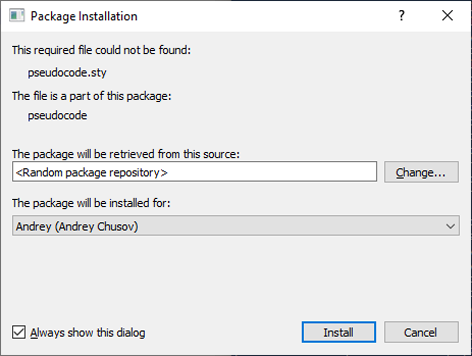
\includegraphics{workbook-extras/miktex-package-installation}
\caption{Автоматическая установка расширений языка \LaTeX, требуемых документом, в процессе его компиляции}
\label{автоустановка расширений miktex}
\end{figure}

\subsection{Среда разработки TeXstudio.}
Несмотря на то, что дистрибутива достаточно для сборки большинства документов, а для полноценного набора текста достаточно стандартного блокнота (хотя Notepad++ \cite{npp} удобнее), для набора документов и автоматизации их сборки можно использовать среды верстки документов \LaTeX.
В настоящем документе кратко описана бесплатная программа TeXstudio, распространяемая для Windows, и облегчающая набор и сборку.
Интерфейс программы представлен на рис. \ref{скриншот texstudio}.
\begin{figure}[ht]
\centering
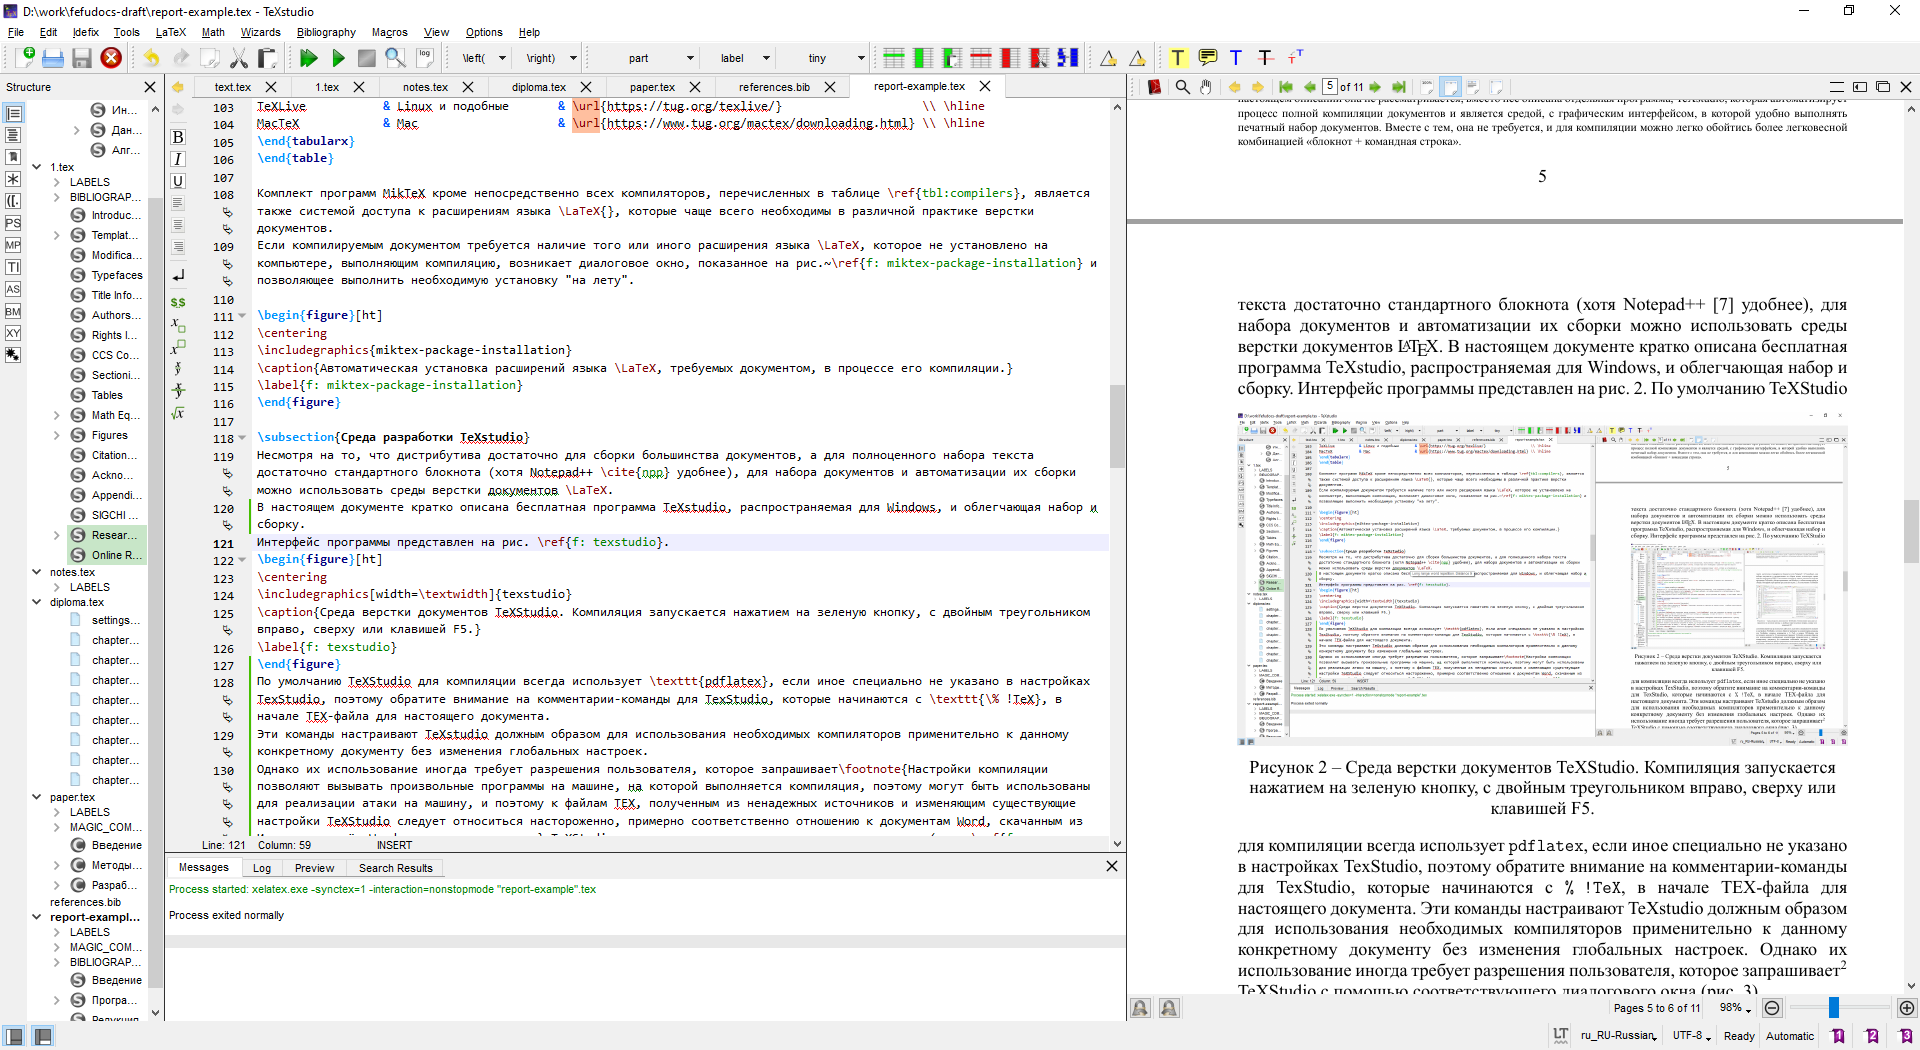
\includegraphics[width=\textwidth]{workbook-extras/texstudio}
\caption{Среда верстки документов TeXstudio. Компиляция запускается нажатием на зеленую кнопку, с двойным треугольником вправо, сверху или клавишей F5}
\label{скриншот texstudio}
\end{figure}
По умолчанию TeXstudio для компиляции всегда использует \texttt{pdflatex}, если иное специально не указано в настройках TeXstudio, поэтому обратите внимание на комментарии-команды для TeXstudio, которые начинаются с \texttt{\% !TeX}, в начале TEX-файла для настоящего документа.
Эти команды настраивают TeXstudio должным образом для использования необходимых компиляторов применительно к данному конкретному документу без изменения глобальных настроек.
Однако их использование иногда требует разрешения пользователя, которое запрашивает\footnote{Настройки компиляции позволяют вызывать произвольные программы на машине, на которой выполняется компиляция, поэтому могут быть использованы для реализации атаки на машину, и поэтому к файлам TEX, полученным из ненадежных источников и изменяющим существующие настройки TeXstudio следует относиться настороженно, примерно соответственно отношению к документам Word, скачанным из Интернет, о чём Word тоже предупреждает.} TeXstudio с помощью соответствующего диалогового окна (рис. \ref{скриншот предупреждения texstudio}).
\begin{figure}
\centering
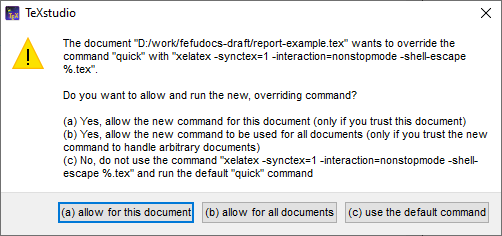
\includegraphics{workbook-extras/texstudio-rules-override}
\caption{Предупреждение TeXstudio о том, что файл TEX запрашивает изменение существующих настроек TeXstudio под себя. Для сборки документа требуется нажать "(a) allow for this document" или "(b) allow for all documents"}
\label{скриншот предупреждения texstudio}
\end{figure}

\section{Написание текста документа}
\subsection{Структура документа.}\label{раздел про структуру документа}
Исходный текст документа в формате \LaTeX{} имеет одну и ту же базовую структуру и состоит из двух основных частей --- преамбулы и тела документа (рис.~\ref{структура документа latex}).

\begin{figure}[ht]
\begin{lstlisting}[language={[LaTeX]TeX}]
%Преамбула
\documentclass[report]{fefudoc} %Класс документа
%Здесь:
% во-первых, с помощью директивы \textbackslash usepackage подключаются требуемые
% расширения, например:
\usepackage{subfig} %по одному
\usepackage{amsfonts, amssymb, amsthm} %или сразу несколько;
% во-вторых, выполняются настройки и параметризация:
\author{ Б8117-09.03.04 }{ Сидоров Иван Петрович } %документа;
\captionsetup[table]{position=top} %расширений
                          % - в данном случае расширения subfig.
%Некоторые расширения можно параметризовать сразу при включении
% в квадратных скобках
\usepackage[caption=false]{subfig}

% Тело документа
\begin{document}
	Привет!
\end{document}
\end{lstlisting}
\caption{Базовая структура документа на языке \LaTeX{}}
\label{структура документа latex}
\end{figure}

\paragraph{Преамбула} приводится в начале \LaTeX-файла, вплоть до директивы \verb+\begin{document}+ и содержит в себе основную и наиболее общую информацию о документе, а именно:
\begin{itemize}
\item категорию и тип документа.
\item используемые для сборки документа расширения языке --- те, что скачиваются при необходимости (при первой сборке, см.~рис.~\ref{автоустановка расширений miktex});
\item настройки и параметры расширений;
\item общую информацию о документе. Например, ФИО автора, его организация, название документа и.~т.~п. Конкретика в данном случае зависит от категории и типа документа, например, диплом или диссертация могут требовать указание научного руководителя, статьи --- ключевых слов.
\end{itemize}

Категория документа чаще всего определяется его классом, который вместе с параметрами указывается в начале с помощью директивы \verb+\documentclass+.
Наиболее распространены классы "article" (статья), "book" (книга), "proc" (материалы конференций) и другие.
Список наиболее распространенных классов приведен в \cite{ctan-standard-latex-classes}.\
Некоторые из этих классов (например, article, book, proc, letter) являются стандартными и устанавливаются на компьютер вместе с дистрибутивом \LaTeX{}.
Другие, в том числе распространенные (такие как "IEEEtran", "IEEEconf" журналов IEEE, "llncs" и "sn-jnl" у Springer, "acmart" у ACM), представлены в виде классов, хранящихся в файлах, обычно с расширением "CLS".
Это обычные текстовые файлы, содержащие правила компоновки документов, которые скачиваются с сайтов издательств. Чаще всего эти классы параметризуются значениями в квадратных скобках.

Таким файлом является и файл "fefudoc.cls", реализующий одноименный класс "fefudoc", которому принадлежит настоящий документ.

Например, чтобы создать доклад класса "fefudoc", необходимо начать документ с объявления его класса "fefudoc" (в фигурных скобках), указав при этом параметр "report" (в квадратных скобках) с помощью директивы
\begin{lstlisting}[language={[LaTeX]{TeX}}]
\documentclass[report]{fefudoc}
\end{lstlisting}

После объявления класса документа с помощью директив \verb+\usepackage+ указываются требуемые расширения языка \LaTeX{}.
Расширений существует большое множество, они решают совершенно разные задачи, и их выбор определяется автором документа по мере необходимости.
Все стандартные расширения бесплатны, дистрибутив MikTeX скачивает их по требованию документом после разрешения автором (см. рис. \ref{автоустановка расширений miktex}).

Популярными являются такие расширения, как \texttt{amsmath} и \texttt{mathtools}, предоставляющие гибкие инструменты для написания формул; \texttt{geometry} для гибкой установки геометрии документа (например, размер листа, поля, ориентация), \texttt{fontspec} для установки параметров используемых шрифтов, \texttt{graphicx} и \texttt{adjustbox} для манипуляций с включаемыми рисунками, \texttt{tikz} для рисования прямо в \LaTeX{}, \texttt{xcolor} для задания цвета текста, \texttt{url} для включения Интернет-ссылок, \texttt{tabularx} для гибкости работы с таблицами, \texttt{algorithm2e} для описания алгоритмов, \texttt{biblatex} для автоматизации создания и поддержки списков литературы и множество других.

Дистрибутив MikTeX предоставляет консоль (рис.~\ref{Консоль MikTeX}) для поиска, ручной установки, удаления и обновления требуемых расширений языка.
\begin{figure}[ht]
\centering
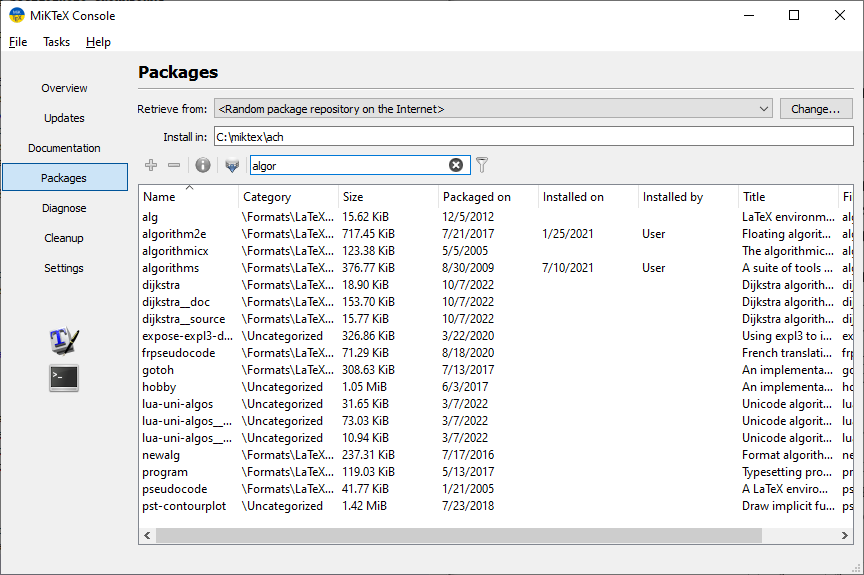
\includegraphics[width=12cm]{workbook-extras/miktex-console}
\caption{Консоль MikTeX для управления и ручной установки расширений \LaTeX{}}
\label{Консоль MikTeX}
\end{figure}
Также расширения \LaTeX{} могут поставляться в текстовых файлах, обычно имеющих тип "STY".
Некоторые расширения могут предоставлять возможность кастомизации предоставляемых функций указанием параметров, также в квадратных скобках или с помощью специальных директив, которые реализуются расширением (см.~рис.~\ref{структура документа latex}).
Например, расширение \texttt{biblatex} с помощью директивы \verb+\addbibresource+, указываемой в преамбуле, требует указания файла со списком литературы.

В преамбуле доклада "report" документа "fefudoc" указывается следующая информация.

\begin{itemize}
\item \texttt{\textbackslash location} --- город, в котором создан (собран, опубликован) документ: например,
\texttt{\textbackslash location\{Владивосток\}};
\item \texttt{\textbackslash Institute} --- институт ДВФУ, в котором обучается автор документа: например, \texttt{\textbackslash Institute\{Политехнический институт (Школа)\}};
\item \texttt{\textbackslash Department} --- департамент или кафедра, обучающая автора документа: например, \texttt{\textbackslash Department\{Департамент электроники, телекоммуникации и приборостроения\}};
\item \texttt{\textbackslash specialty} --- специальность автора реферата, например, \texttt{\textbackslash specialty\{09.03.04\}{[Программная инженерия]}};
второй параметр, в квадратных скобках опционален, если его опустить класс \texttt{fefudoc} попытается самостоятельно расшифровать специальность согласно общероссийскому классификатору 009-2016 и учебному плану, например: \texttt{\textbackslash specialty\{09.03.04\}};
\item \texttt{\textbackslash profile} --- профиль, по которому обучается автор, например \texttt{\textbackslash profile\{Системы радиосвязи и радиодоступа\}};
\item \texttt{\textbackslash discipline} --- дисциплина, по которой подготовлен реферат, например, \texttt{\textbackslash discipline\{Параллельное программирование\}};
\item \texttt{\textbackslash author} --- группа и ФИО автора, например, \texttt{\textbackslash author\{Б3121-11.03.02втц\}\{Сидоров Иван Петрович\}};
\item \texttt{\textbackslash teacher} --- учёная степень, учёное звание, должность и ФИО преподавателя по дисциплине, например, \texttt{\textbackslash teacher\{доктор физико-математических наук\}\{доцент\}\{профессор каф. ЭТиП\}\{Петров Петр Петрович\}};
\item \texttt{\textbackslash title} --- наименование (тема) работы, например, \texttt{\textbackslash title\{Использование \textbackslash LaTeX\{\}\ для написания рефератов\}};
\item \texttt{\textbackslash year} --- год написания работы, например \texttt{\textbackslash year=2023}. Если не указывать, то для получения года используется текущее время на компьютере, на котором выполняется сборка документа.
\end{itemize}

\paragraph{Тело документа} содержит в себе его основное наполнение.
Часто, но не всегда, тело документа начинается с директивы \texttt{\textbackslash frontmatter}, которая указывает на необходимость создать титульную страницу в начале собранного документа.
Остальной текст структурируется согласно требованиям организации, в которую сдается документ, и класса документа.
Например, тело реферата \texttt{fefudoc} начинается с директив
\begin{lstlisting}[language={[LaTeX]{TeX}}]
\frontmatter % заглавная страница
\tableofcontents % оглавление
\end{lstlisting}

Далее тело может содержать части (директива \texttt{\textbackslash part} для книг классов \texttt{book}), главы (для дипломов и диссертаций ДВФУ, а также для стандартных классов \texttt{book} и \texttt{report} доступна директива \texttt{\textbackslash chapter}), разделы (директива \texttt{\textbackslash section}), подразделы (директива \texttt{\textbackslash subsection}), под-подразделы (директива \texttt{\textbackslash subsubsection}), параграфы (\texttt{\textbackslash paragraph}) и подпараграфы (\texttt{\textbackslash subparagraph}) (рис. \ref{разделы-подразделы}\footnote{Пробелы возле фигурных скобок не требуются. Расстановка их на рисунке обусловлена тем, что нелатинские алфавиты плохо поддерживаются расширением \texttt{\footnotesize listings}, используемым здесь для отображения исходного кода на \LaTeX{}. Подробности в разделе \ref{раздел про исходный код}.}).
\begin{figure}[ht]
\begin{lstlisting}[language={[LaTeX]{TeX}}, literate={-}{-}1]
\section{ Заголовок раздела }
 Текст раздела.

 Следующий абзац раздела.
 Ссылка на раздел \ref{ содержимое label адресуемого раздела }.
\subsection{ Подраздел }
 Текст подраздела.
\subsubsection{ Под-подраздел }
 Текст под-подраздела.
\paragraph{ Параграф }
 Текст.
\subparagraph{ Подпараграф }
 Текст.
\section{ Заголовок следующего раздела }
 \label{ содержимое label адресуемого раздела }
 Текст следующего раздела.
\end{lstlisting}
\caption{Структура документа}
\label{разделы-подразделы}
\end{figure}

Обычно разделы, подразделы и под-подразделы тем или иным образом нумеруется, и на них можно при необходимости сослаться с помощью директивы \texttt{\textbackslash ref}, если задан маркер \texttt{\textbackslash label}, как указано в разделе \ref{раздел про ссылки внутри документа}.
Вместе с этим, некоторые специальные главы или разделы, например, введение, часто требуется не нумеровать.
Такие разделы создаются с помощью директив со звездочкой, например
\begin{lstlisting}[language={[LaTeX]{TeX}}]
\section*{ Ненумеруемый раздел }
\end{lstlisting}

Дополнительно, часто документы должны оканчиваться специальными разделами, и для таких разделов существуют свои, специальные, директивы.
Например, выпускные квалификационные работы и рефераты должны в конце содержать список литературы.
Расширение \texttt{biblatex} (см. раздел \ref{раздел про списки литературы}), которое может быть использовано для управления списками литературы, предоставляет директиву \texttt{\textbackslash printbibliography}, которая "вставляет" список в соответствующее место документа.
Также достаточно часто в конце документа требуется наличие содержания (вместо оглавления), предметного указателя, списков рисунков, глоссария, приложений.

Более подробная информация об определении структуры документа доступна на английском языке в \cite{wikibooks-document-structure}.

\subsection{Форматирование текста}
\subsubsection{Директивы и области их действия.}\label{раздел про директивы}
Директивы (команды) \LaTeX{} задаются с обратным слешем вначале: например \texttt{\textbackslash LaTeX}.

Некоторые из таких команд принимают обязательные параметры в фигурных скобках справа, например, курсивный текст может быть задан командой \texttt{\textbackslash textit}, которая принимает в качестве параметра выделяемый текст: например, \texttt{этот \textbackslash textit\{текст выделен курсивом\}, а этот --- нет} производит при компиляции строку "этот \textit{текст выделен курсивом}, а этот --- нет".

Область действия директив, в зависимости от конкретной директивы, может быть одного из трех типов.

Первый --- это действие директивы в отношение своего параметра, как это указано выше на примере директивы \texttt{\textbackslash textit}.

Второй --- это действие директив-переключателей. Действие директивы-переключателя начинается с места, в котором, в исходном коде, эта директива указана, и до встречи в исходном тексте одного из двух событий.
Во-первых, действие директивы может быть заменено действием альтернативной директивы-переключателя, например, \texttt{этот \textbackslash itshape текст выделен курсивом, \textbackslash normalfont а этот --- нет} компилируется в "этот \itshape текст выделен курсивом, \normalfont а этот --- нет".
Во-вторых, действие директивы-переключателя может ограничиваться фигурными скобками, в которых эта директива использована, например, \texttt{\{этот \textbackslash itshape текст выделен курсивом,\} а этот --- нет} компилируется в "{этот \itshape текст выделен курсивом,} а этот --- нет".

Третий тип --- это то, что в \LaTeX{} называется окружением (\textit{environment}).
Окружения обычно используются, когда их эффект нужно распространить на сравнительно большой участок файла \LaTeX{} и применяются в основном для создания специальных блоков документа, таких как рисунки, формулы или таблицы.
Окружения являются более составными управляющими элементами языка \LaTeX{}, чем директивы и задаются двумя директивами --- начала окружения \texttt{\textbackslash begin\{\textit{имя окружения}\}}, и его конца \texttt{\textbackslash end\{\textit{имя окружения}\}}.
Например, нумерованная формула в \LaTeX{} может быть задана окружением "equation" (см. разд.~\ref{раздел про формулы}) следующим образом:
\begin{verbatim}\begin{equation}
E = m c^2
\end{equation}\end{verbatim}
что компилируется в
\begin{equation}
E = m c^2
\end{equation}

Специальной является директива, задающая однострочный комментарий (многострочных комментариев в \LaTeX{} нет).
Эта директива задается символом процента "\%" и приводит к тому, что часть строки после процента, включая сам процент и перенос строки, игнорируется компилятором \LaTeX{}, например
\begin{lstlisting}[language={[LaTeX]{TeX}}]
 Это нормальный текст. %А это игнорируемый комментарий.
\end{lstlisting}

\subsubsection{Использование специальных символов в тексте.}\label{раздел про специальные символы}
Для отображения в тексте специальных символов, используемых для определения команды, используются специальные контрольные последовательности.

Большинство специальных символов можно отображать в тексте как обычные символы, предваряя их обратным слешем.
Например, отобразить процент в тексте можно с помощью \texttt{\textbackslash \%}, что компилируется в символ "\%".
Аналогично фигурные скобки можно отображать с помощью \texttt{\textbackslash\{\textbackslash\}}, что создает строку "\{\}".
Исключениями являются обратный слеш~"\textbackslash", т\'{и}льда~"\~{}" и к\'{а}рет~"\^{}".

Обратный слеш отображается с помощью директивы \texttt{\textbackslash textbackslash} в обычном режиме и с помощью \texttt{\textbackslash backslash} --- в режиме ввода формул (см. разд.~\ref{раздел про формулы}).

Тильда отображается с помощью обратного слеша и следующей за ним пары фигурных скобок: \texttt{\textbackslash \~{}\{\}} отображается как "\~{}".

Специальными символами, отображение которых в \LaTeX{} требуется выполнять указанными способами, являются следующие.
\begin{itemize}
\item Доллар "\$". Отображается с помощью \texttt{\textbackslash \$}.
\item Решетка "\#". Отображается с помощью \texttt{\textbackslash \#}.
\item Процент "\%". Отображается с помощью \texttt{\textbackslash \%}.
\item Амперсанд "\&". Отображается с помощью \texttt{\textbackslash \&}.
\item Символ подчеркивания "\_". Отображается с помощью \texttt{\textbackslash \_}.
\item Левая фигурная скобка "\{". Отображается с помощью \texttt{\textbackslash \{}.
\item Правая фигурная скобка "\}". Отображается с помощью \texttt{\textbackslash \}}.
\item Карет "\^{}". Отображается с помощью \texttt{\textbackslash \^{}\{\}}.
\item Тильда "\~{}". Отображается с помощью \texttt{\textbackslash \~{}\{\}}.
\item Обратный слеш "\textbackslash". Отображается с помощью \texttt{\textbackslash textbackslash}.
\end{itemize}

\subsubsection{Абзацы и новые строки.}\label{подраздел про абзацы}
Один перенос строки в \LaTeX{} имеет эффект, эквивалентный постановке пробела.
Например,
\begin{verbatim}
"Этот текст
и этот текст.
И даже этот текст."
\end{verbatim}
компилируются в один абзац и производят текст:

"Этот текст
и этот текст.
И даже этот текст."

Абзацы отделяются друг от друга пустыми строками. Например,
\begin{verbatim}
это один абзац,

а это --- другой,
\end{verbatim}
что производит эффект:

это один абзац,

а это --- другой,

Исключением из этого правила являются структурные директивы из раздела \ref{раздел про структуру документа}: любая из них начинает новый абзац, даже если она задана посреди предложения.

Методом принудительного переноса строки, который используется при написании многострочных формул, матриц и таблиц, является последовательность из двух обратных слешей "\texttt{\textbackslash\textbackslash}".
Например, \texttt{этот текст\\разделен на две строки} компилируется в "этот текст\\разделен на две строки".

В редких случаях может возникать необходимость начать текст нового абзаца или раздела на новой странице.
Для этих целей в \LaTeX{} существует специальная директива \verb+\clearpage+, отчищает остаток текущей страницы документа от любого текста, то есть переносит весь последующий текст на следующую страницу, что может быть удобным, например, если некоторые компоненты документа должны начинаться в начале страницы.

\subsubsection{Пробелы.}
Существует два основных типа пробела: обычный и неразрывный.

Обычный разделяет слова обычным образом и допускает перенос строк компилятором \LaTeX{} в месте пробела.
Несколько пробелов всегда заменяются при компиляции одним.
Если пробел следует за какой-нибудь директивой, то пробел "съедается" директивой и отбрасывается.

Например, строка \texttt{\textbackslash LaTeX компилирует} будет собрана в строку "\LaTeX компилирует".
В таких случаях после команды необходимо использовать фигурные скобки: \texttt{\textbackslash LaTeX\{\} компилирует} собирается в "\LaTeX{} компилирует".

Неразрывный пробел используется для постановки пробела в месте, в котором необходимо запретить компилятору перенос строки.
Для в исходном коде \LaTeX{} установка неразрывных пробелов осуществляется тильдой "\~{}".
Например, \texttt{рис.\~{}1} соберется в строку "рис.~1", но тильда гарантирует, что разрыва строк не будет между "рис." и "1"\footnote{Точнее, разрыв не более вероятен, чем разрыв посреди слова}.

Использование неразрывного пробела обычно ограничено специальными случаями: например, может быть нежелательным перенос строк между фамилиями и инициалами, а также в ссылках типа "рис.~1" или "разд.~1".

\subsubsection{Выделение текста.}\label{раздел про выделение текста}
Директивы выделения текста, включая их переключательные альтернативы, приведены в таблице~\ref{таблица с методами выделения текста}.
Наиболее часто применяемые из них --- это курсив (директивы \texttt{\textbackslash textit} и \texttt{\textbackslash itshape}), а также жирное начертание (директивы \texttt{\textbackslash textbf} и \texttt{\textbackslash bfseries}).

\begin{longtable}{|c|c|p{.52\textwidth}|}
\caption{Директивы для выделения текста}\label{таблица с методами выделения текста}\endfirsthead\endhead
\hline
\thead{Директива} & \thead{Директива-\\переключатель} & \thead{Эффект} \\
\hline
\texttt{\textbackslash textit} & \texttt{\textbackslash itshape} & Выделение текста курсивом. Например, \texttt{\textbackslash textit\{курсивный текст\}} производит \textit{курсивный текст}; \texttt{\{\textbackslash itshape курсивный текст\}} производит {\itshape курсивный текст}.\\
\hline
\texttt{\textbackslash textbf} & \texttt{\textbackslash bfseries} & Выделение текста жирным начертанием. Например, \texttt{\textbackslash textbf\{жирный текст\}} производит \textbf{жирный текст}; \texttt{\{\textbackslash bfseries жирный текст\}} производит {\bfseries жирный текст}. \\
\hline
\texttt{\textbackslash textsf} & \texttt{\textbackslash sffamily} & Выделение текста, используя шрифт с начертанием одинаковой толщины, например, шрифтом "Arial". Например, \texttt{\textbackslash textsf\{текст\}} производит \textsf{текст}; \texttt{\{\textbackslash sffamily текст\}} производит {\sffamily текст}. \\
\hline
\texttt{\textbackslash texttt} & \texttt{\textbackslash ttfamily} & Выделение текста, используя шрифт, в котором все символы имеют одинаковую ширину, например, шрифтом "Consolas". Часто используется в документах для начертания кода программ, вывода терминала и~т.~п. Например, \texttt{\textbackslash texttt\{текст\}} производит \texttt{текст}; \texttt{\{\textbackslash ttfamily текст\}} производит {\ttfamily текст}. \\
\hline
\texttt{\textbackslash textsc} & \texttt{\textbackslash scshape} & Выделение текста малыми прописными --- так, что все его буквы пишутся как прописные, но имеют размер такой же как строчные.
Не все шрифты поддерживают такое начертание: \textit{таким, например, шрифт "Liberation Serif", используемый при компиляции документов класса fefudoc в Linux}.
Если начертание малыми прописными не поддерживается, при компиляции текста, помеченного с помощью \texttt{\textbackslash textsc} или \texttt{\textbackslash scshape}, будет выведено соответствующее предупреждение, а текст будет отображен с нормальным начертанием \texttt{\textbackslash textnormal}.
Если же начертание поддерживается, то \texttt{\textbackslash textsc\{текст строчными буквами\}} производит \textsc{текст строчными буквами}; \texttt{\{\textbackslash scshape текст строчными буквами\}} производит {\scshape текст строчными буквами}. \\
\hline
\texttt{\textbackslash textsl} & \texttt{\textbackslash slshape} & Выделение текста наклонным начертанием. Часто это то же самое, что и курсив, но некоторые шрифты предлагают оба варианта: курсив обычно более каллиграфичный, в то время как наклонное начертание выглядит как обычный текст, написанный под углом. Например, \texttt{\textbackslash textsl\{наклонный текст\}} производит \textsl{наклонный текст}; \texttt{\{\textbackslash slshape наклонный текст\}} производит {\slshape наклонный текст}. \\
\hline
\texttt{\textbackslash textnormal} & \texttt{\textbackslash normalfont} & Изменение начертания текста на нормальное: то есть отмена всех выделений. Например, \texttt{\textbackslash textbf\{ текст \textbackslash textnormal\{нормальный текст\} текст} производит \textbf{текст \textnormal{нормальный текст} текст}; \texttt{\{\textbackslash bfseries текст \textbackslash normalfont нормальный текст \textbackslash bfseries текст\}} производит {\bfseries текст \normalfont нормальный текст \bfseries текст}. \\
\hline
\end{longtable}

В дополнение к указанным директивам существует директива \texttt{\textbackslash emph} (и её переключательная альтернатива \texttt{\textbackslash em}).
Эта директива, в отличие от указанных в таблице \ref{таблица с методами выделения текста}, семантическая: она выделяет текст \emph{каким-то} образом --- тем, который определён классом документа, и является в некотором смысле интеллектуальной.
Например, использование вложенного выделения с помощью одной из директив таблицы \ref{таблица с методами выделения текста} не имеет смысла: директивы \texttt{\textbackslash textit\{это выделенный, \textbackslash textit\{а это еще более выделенный\} текст\}} будет скомпилирован в \textit{это выделенный, \textit{а это еще более выделенный} текст}.
В противоположность этому директивы \texttt{\textbackslash emph\{это выделенный, \textbackslash emph\{а это еще более выделенный\} текст\}} будет скомпилирован относительно корректно в \emph{это выделенный, \emph{а это еще более выделенный} текст}.

Также текст можно подчеркивать с помощью директивы \texttt{\textbackslash underline}, например, \texttt{\textbackslash underline\{подчеркнутый текст\}} компилируется в \underline{подчеркнутый текст}.

Существуют и другие способы выделения теста.
Например, расширение \texttt{soul} языка \LaTeX позволяет выполнять выделение цветом.
Однако по состоянию версии 3.1 от 14.06.2023 его использование с нелатинскими алфавитами имеет проблемы.

Класс \texttt{fefudoc} также предоставляет команду \texttt{\textbackslash todo}, которая принимает в качестве параметра строку и, если класс \texttt{fefudoc} использован с параметром \texttt{draught} (например, \texttt{\textbackslash documentclass[report, draught]\{fefudoc\}}, см. раздел \ref{раздел про структуру документа}), отображает эту строку параметр, при компиляции маркируя её желтым цветом; а если параметр \texttt{draught} не использован, то при компиляции генерируется ошибка с указанием места с \texttt{\textbackslash todo} в документе.
Пример использования: \verb+\todo{не забыть добавить список литературы}+.

Начертание текста также можно выполнять в верхнем и нижнем индексе.
Для этого соответственно используются директивы \texttt{\textbackslash textsuperscript} и \texttt{\textbackslash textsubscript}.
Например, текст может быть представлен в \textsuperscript{верхнем} и \textsubscript{нижнем} индексах.

\subsubsection{Минус, дефисы, знаки диапазона и тире.}\label{раздел про дефис}
Существуют четыре знака, обозначаемых горизонтальной чертой, и их начертание отличается длиной, также как и пробелы вокруг них.

Во-первых, это знак минус.
Знак минус проставляется только в режиме ввода формул \LaTeX (см. раздел \ref{раздел про формулы}).
Например, \texttt{\$-4\$} компилируется в $-4$, а \texttt{\$5-4\$} компилируется в $5 - 4$.

Во-вторых, это дефис.
Его использование задается в файле \LaTeX{} одним символом "-".
Например, \texttt{делали-недоделали} компилируется в делали-недоделали.

В-третьих, это более длинный знак диапазона, который обозначается в файле \LaTeX{} двумя дефисами: "\verb+--+".
Например, текст \verb+даты проведения конференции: 11.09.2023--13.09.2023+ компилируется в текст "даты проведения конференции: 11.09.2023--13.09.2023".

В-четвертых, это наиболее длинное тире, которое записывается в файле \LaTeX{} тремя дефисами.
Например, \verb+тире --- наиболее длинная из всех горизонтальных черточек+ компилируется в "тире --- наиболее длинная из всех горизонтальных черточек".

\subsection{Списки.}
Существует три основных вида списков \LaTeX{}: маркированные, нумерованные и определительные.
Все виды списков задаются соответствующими окружениями (см. раздел \ref{раздел про директивы}) --- \texttt{itemize}, \texttt{enumerate} и \texttt{description}, а пункты всех этих списков обозначаются директивой \texttt{\textbackslash item}.

\subsubsection{Маркированные списки} определяются в окружении \texttt{itemize}.
Например, код
\begin{verbatim}
\begin{itemize}
\item Пункт 1.
\item Пункт 2.
\item Пункт 3.
\end{itemize}
\end{verbatim}
компилируется в маркированный список
\begin{itemize}
\item Пункт 1.
\item Пункт 2.
\item Пункт 3.
\end{itemize}

\subsubsection{Нумерованные списки}\label{раздел про нумерованные списки}
задаются окружением \texttt{enumerate}, например,
\begin{verbatim}
\begin{enumerate}
\item Пункт 1.
\item Пункт 2.
\item Пункт 3.
\end{enumerate}
\end{verbatim}
компилируется в нумерованный список
\begin{enumerate}
\item Пункт 1.
\item Пункт 2.
\item Пункт 3.
\end{enumerate}

Расширением \texttt{enumitem} \cite{enumitem} предоставляется возможность кастомизировать нумерованные списки указанием, в качестве опционального параметра, паттерна, согласно которому нумеруются элементы.
В этом паттерне для указания места, в которое подставляется номер элемента, используются директивы (с астериском "*" на конце) \verb+\arabic*+ для использования арабских цифр; \verb+\Roman*+ для использования прописных римских цифр и \verb+\roman*+ --- строчных; \verb+\Alph*+ для использования прописных, и \verb+\alph*+ --- строчных, букв алфавита, используемого в языке, на котором написан документ.

Например, список, заданный в \LaTeX{} кодом
\begin{verbatim}
\begin{enumerate}[label=\arabic*)]
\item пункт 1;
\item пункт 2;
\item пункт 3.
\end{enumerate}
\end{verbatim}
в результате компиляции становится\footnote{Обратите внимание на то, что в русскоязычных документах списки, номера которых отделяются закрывающей скобкой, принято делать частью окружающих их предложений, поэтому элементы таких списков нужно начинать со строчных символов (кроме специальных случаев, например, аббревиатур), и все элементы, кроме, возможно, последнего, не нужно оканчивать точкой.}
\begin{enumerate}[label=\arabic*)]
\item пункт 1;
\item пункт 2;
\item пункт 3.
\end{enumerate}
Список
\begin{verbatim}
\begin{enumerate}[label=\textit{\Alph*}.]
\item Пункт 1.
\item Пункт 2.
\item Пункт 3.
\end{enumerate}
\end{verbatim}
становится
\begin{enumerate}[label=\textit{\Alph*}.]
\item Пункт 1.
\item Пункт 2.
\item Пункт 3.
\end{enumerate}

\subsubsection{Определительные списки}
задаются окружением \texttt{description}, а директива \texttt{\textbackslash item}, указанная в них, принимает в квадратных скобках параметр --- то, что определяется в соответствующем пункте. Например
\begin{verbatim}
\begin{description}
\item [Реферат] содержит краткое, на 8--15 страниц, описание
исследованной студентом технологии, метода, модели или научно-
технической проблемы. Обычно целью реферата является
демонстрация обучающимся перед проверяющим собственных знаний
и умений по теме работы.
\item [Научная статья] содержит небольшое, обычно на 5--15
страниц, описание исследованной проблемы и/или разработанного
автором метода её решения. В отличие от реферата, целью научной
статьи является опубликование нового знания, то есть научная
статья должна обладать научной новизной.
\item [Бакалаврский диплом] содержит полное и развернутое
описание разработки или исследования, выполненного самостоятельно
студентом, имеющего научную новизну или практическую ценность.
Задача студента, пишущего диплом, --- продемонстрировать
собственные знания и умения, полученные в процессе обучения по
своей специальности, для решения реальных прикладных или
теоретических задач соответствующей предметной области.
\item [Магистерская диссертация] содержит полное и развернутое
описание научно-исследовательской работы, выполненной
магистрантом за время обучения в магистратуре. В отличие от
бакалаврского диплома, магистерская диссертация является научной
работой, то есть прежде всего должна обладать научной новизной,
неся в себе таким образом новое знание по исследуемой проблеме,
а использованные методы исследования должны быть научными ---
опираться на знания в реферируемых источниках, формальные
теоретические и экспериментальные доказательства.
\end{description}
\end{verbatim}
компилируется в
\begin{description}
\item [Реферат] содержит краткое, на 8--15 страниц, описание
исследованной студентом технологии, метода, модели или научно-
технической проблемы. Обычно целью реферата является
демонстрация обучающимся перед проверяющим собственных знаний
и умений по теме работы.
\item [Научная статья] содержит небольшое, обычно на 5--15
страниц, описание исследованной проблемы и/или разработанного
автором метода её решения. В отличие от реферата, целью научной
статьи является опубликование нового знания, то есть научная
статья должна обладать научной новизной.
\item [Бакалаврский диплом] содержит полное и развернутое
описание разработки или исследования, выполненного самостоятельно
студентом, имеющего научную новизну или практическую ценность.
Задача студента, пишущего диплом, --- продемонстрировать
собственные знания и умения, полученные в процессе обучения по
своей специальности, для решения реальных прикладных или
теоретических задач соответствующей предметной области.
\item [Магистерская диссертация] содержит полное и развернутое
описание научно-исследовательской работы, выполненной
магистрантом за время обучения в магистратуре. В отличие от
бакалаврского диплома, магистерская диссертация является научной
работой, то есть прежде всего должна обладать научной новизной,
неся в себе таким образом новое знание по исследуемой проблеме,
а использованные методы исследования должны быть научными ---
опираться на знания в реферируемых источниках, формальные
теоретические и экспериментальные доказательства.
\end{description}

\subsubsection{Вложенные списки.}
Когда требуется вложенность списков, в соответствующем пункте, который, как указано выше, начинается с директивы \verb+\item+, можно также использовать одно из перечисленных окружений.
Например,
\begin{verbatim}
\begin{itemize}
 \item пункт 1;
 \item пункт 2;
 \begin{itemize}
  \item подпункт 1;
  \item подпункт 2;
  \begin{itemize}
   \item под-подпункт 1;
   \item под-подпункт 2;
   \begin{itemize}
    \item под-под-подпункт 1;
    \item под-под-подпункт 2;
   \end{itemize}
  \end{itemize}
  \item подпункт 3;
 \end{itemize}
 \item пункт 3.
\end{itemize}
\end{verbatim}
Уровень вложенности автоматически учитывается при компиляции таких составных списков и обозначении их элементов.
Так указанный пример компилируется в
\begin{itemize}
 \item пункт 1;
 \item пункт 2;
 \begin{itemize}
  \item подпункт 1;
  \item подпункт 2;
  \begin{itemize}
   \item под-подпункт 1;
   \item под-подпункт 2;
   \begin{itemize}
    \item под-под-подпункт 1;
    \item под-под-подпункт 2;
   \end{itemize}
  \end{itemize}
  \item подпункт 3;
 \end{itemize}
 \item пункт 3.
\end{itemize}

Кастомизация отображения вложенных нумерованных списков расширением \texttt{enumitem} достигается путём указания паттерна представления номера на каждом уровне вложенности.
Для того, чтобы задать паттерн, используются те же директивы из раздела~\ref{раздел про нумерованные списки}: \verb+\arabic+ для представления номера арабскими цифрами, \verb+\Roman+ и \verb+\roman+ --- для представления соответственно прописными и строчными римскими цифрами, \verb+\Alph+ и \verb+\alph+ --- для представления номера соответственно прописными и строчными символами алфавита языка, на котором создается документ \LaTeX{}.
Однако здесь данные директивы, во-первых, применяются без астериска "*", а во-вторых, принимают в качестве обязательного параметра наименование номера в списке: \texttt{enumi}, \texttt{enumii}, \texttt{enumiii} или \texttt{enumiv}.
Эти наименования образованы словом "enum" и постфиксом --- номером уровня вложенности, заданным строчными римскими цифрами от 1 до 4.
Например, код
\begin{verbatim}
\begin{enumerate}[label=\Roman{enumi}]
 \item пункт 1;
 \item пункт 2;
 \begin{enumerate}[label=\arabic{enumii}]
  \item подпункт 1;
  \begin{enumerate}[label=\arabic{enumii}\Alph{enumiii}.]
   \item под-подпункт 1;
   \item под-подпункт 2;
   \begin{enumerate}[
    label=\arabic{enumii}\Alph{enumiii}-\alph{enumiv})]
    \item под-под-подпункт 1;
    \item под-под-подпункт 2;
   \end{enumerate}
  \end{enumerate}
  \item подпункт 2;
 \end{enumerate}
 \item пункт 3;
 \item пункт 4.
\end{enumerate}
\end{verbatim}
компилируется в список
\begin{enumerate}[label=\Roman{enumi}]
 \item пункт 1;
 \item пункт 2;
 \begin{enumerate}[label=\arabic{enumii}]
  \item подпункт 1;
  \begin{enumerate}[label=\arabic{enumii}\Alph{enumiii}.]
   \item под-подпункт 1;
   \item под-подпункт 2;
   \begin{enumerate}[
    label=\arabic{enumii}\Alph{enumiii}-\alph{enumiv})]
    \item под-под-подпункт 1;
    \item под-под-подпункт 2;
   \end{enumerate}
  \end{enumerate}
  \item подпункт 2;
 \end{enumerate}
 \item пункт 3;
 \item пункт 4.
\end{enumerate}

Отметим, что расширение \texttt{enumitem} позволяет с помощью директивы \verb+\setlistdepth+ увеличить максимально возможный уровень вложенности, как это указано в \cite{enumitem}, а также, с помощью директив \verb+\newlist+ и \verb+\setlist+ создавать собственные списки соответственно паттернам, определённым в преамбуле документа.

Альтернативным средством кастомизации вложенных списков является расширение \texttt{easylist} \cite{easylist}.

\subsection{Формулы.}\label{раздел про формулы}
\LaTeX{} может работать в одном из двух основных\footnote{На самом деле режимов больше, они касаются деталей компиляции файла \LaTeX{} и не описаны в данном документе. Например, аспекты размещения абзацев, рисунков и таблиц в тексте реализуются в "вертикальном" режиме, а аспекты расстановки пробелов и слов в предложениях --- в "горизонтальном" режиме \LaTeX{}.} режимов --- в режиме ввода обычного текста и в режиме ввода формул.

В настоящем документе под формулами понимаются математические формулы, иные не описаны, хотя реализуются языком и его расширениями.
Например, химические формулы реализуются расширениями \texttt{chemfig}, \texttt{chemformula} и \texttt{xymtex}.

\subsubsection{Встраиваемые и выносимые формулы.}\label{подраздел про встраиваемые и выносимые формулы}
Формулы \LaTeX{} бывают встраиваемые в основной текст и выносимыми в отдельный блок.
Встраиваемые формулы являются частью обычных предложений, а вход и выход из режима набора формул осуществляется с помощью знака \texttt{\$} или с помощью комбинаций \texttt{\textbackslash (} --- для входа; и \texttt{\textbackslash )} --- для выхода.
Например, и \verb+$z= x y$+, и \verb+\(z =xy\)+ компилируются в одну и ту же формулу $z = x y$. Обратите внимание на то, что пробелы внутри математических формул, написанных в \LaTeX{}, игнорируются и расставляются компилятором \LaTeX{} по-своему, в соответствии с нормативами принятыми в математике.
Исключения составляют некоторые специальные случаи, например, когда часть математической формулы является параметром директивы \texttt{\textbackslash text}.

Формул, которые выносятся в отдельный блок, бывают много видов в зависимости от их размера, вариантов нумерации и выравнивания в многострочных формулах.
Простейшим видом является ненумерованная выносимая формула, которая обрамляется последовательностью "\$\$" (для вхождения и выхода из режима набора формул) или \texttt{\textbackslash [} (для вхождения) и \texttt{\textbackslash ]} (для выхода).
Например, и \verb|$$\sin^2 x + \cos^2 x = 1$$|, и \verb|\[\sin^2 x + \cos^2 x = 1\]| компилируются в $$\sin^2 x + \cos^2 x = 1.$$

Дополнительные методы включения в текст выносимых формул предоставляются расширением \texttt{mathtools} (точнее расширением \texttt{amsmath}, которое опосредованно включается и в некоторых случаях исправляется и улучшается расширением \texttt{mathtools}).

Формулы, выносимые с помощью \texttt{mathtools}, вносятся в необходимые окружения
Основных окружений три: \texttt{equation}, \texttt{gather} и \texttt{align},
и каждое сопровождается версией со "звездочкой": соответственно \texttt{equation*}, \texttt{gather*} и \texttt{align*}.
Версии без звездочки добавляют к формулам нумерацию, и на эти формулы, также как на разделам, можно ссылаться по тексту, используя имя, заданное для формулы директивой \texttt{\textbackslash label}, а сами ссылки задавать, используя директиву \texttt{\textbackslash ref}  --- хотя предпочтительнее для ссылок на формулы использовать специальную директиву \texttt{\textbackslash eqref}, которая автоматически форматирует ссылку в соответствии с общепринятыми нормативами.
Например, задать простейшую нумерованную выносимую формулу и сослаться на неё можно так:
\begin{verbatim}
\begin{equation}\label{второй замечательный предел}
\lim_{n \to \infty} \Big(1 + \frac{1}{n}\Big)^n = e.
\end{equation}
Предел \eqref{второй замечательный предел} называется вторым
замечательным и является одним из определений числа Эйлера $e$.
\end{verbatim}
В результате компиляции такой формулы получается следующий текст:
\begin{equation}\label{второй замечательный предел}
\lim_{n \to \infty} \Big(1 + \frac{1}{n}\Big)^n = e.
\end{equation}
Предел \eqref{второй замечательный предел} называется вторым
замечательным и является одним из определений числа Эйлера $e$.

Очевидно, что вариант \texttt{equation*} со звёздочкой эквивалентен обычным формулам, выносимым с помощью \texttt{\$\$} или \texttt{\textbackslash[} и \texttt{\textbackslash]}, поскольку не проставляет нумерацию.

Длинные формулы иногда требуется разбить на несколько строк.
Для этого \textit{внутри} окружения \texttt{equation} (или внутри \texttt{gather}, или внутри \texttt{align}) можно использовать вложенное окружение \texttt{split} или \texttt{aligned} (не путать с \texttt{align}), задавая точки, по которым выполняется выравнивание строк многострочной формулы, символом \texttt{\&} следующим образом:
\begin{verbatim}
\begin{equation}\label{Возведение в степень по модулю}
\begin{split}
\forall M m_i m_j x n \exists m \Big[&
    m_i \in M \subset \mathbb{N} \\
   &\land m = \prod_{\forall m_k \in M} m_k \\
   &\land x \in \mathbb{Z}_m
    \land n \in \mathbb{Z}
    \land x^n \in \mathbb{Z}_m \\
   &\implies x^n \bmod m_i =  (x \bmod m_i )^n \bmod m_i
\Big]
\end{split}\end{equation}
\end{verbatim}
что компилируется в
\begin{equation}\label{Возведение в степень по модулю}
\begin{split}
\forall M m_i m_j x n \exists m \Big[&
    m_i \in M \subset \mathbb{N} \\
   &\land m = \prod_{\forall m_k \in M} m_k \\
   &\land x \in \mathbb{Z}_m
    \land n \in \mathbb{Z}
    \land x^n \in \mathbb{Z}_m \\
   &\implies x^n \bmod m_i =  (x \bmod m_i )^n \bmod m_i
\Big]
\end{split}\end{equation}
Расширения \texttt{split} и \texttt{aligned} эквивалентны.

Иногда требуется собрать в одну группу несколько индивидуальных формул и, возможно, также индивидуально пронумеровать их.
Для этого служит окружение \texttt{gather} того же расширения \texttt{mathtools}.
Например,
\begin{verbatim}
уравнения \eqref{закон Гаусса}--\eqref{закон Ампера}
\begin{gather}
\label{закон Гаусса}
\oiint_{\partial \Omega} \vec{E} d \vec{S}
  = \frac{1}{\varepsilon_0} \iiint_\Omega \rho dV \\
\label{закон Гаусса о магнитном поле}
\oiint_{\partial \Omega} \vec{B} d \vec{S} = 0 \\
\label{закон Фарадея}
\oint_{\partial \Sigma} \vec{E} d l
  = -\frac{d}{dt} \iint_\Sigma \vec{B} d\vec{S} \\
\label{закон Ампера}
\oint_{\partial\Sigma} \vec{B} dl
  = \mu_0 \Big(\iint_\Sigma \vec{J} d\vec{S}
    + \varepsilon_0 \frac{d}{dt} \iint_\Sigma \vec{E}
       d\vec{S}\Big)
\end{gather}
называются уравнениями Максвелла в интегральной форме и
описывают электромагнитное поле в эквилибриуме, где
уравнение \eqref{закон Гаусса} называется законом Гаусса
об электрическом потоке, уравнение \eqref{закон Гаусса о
магнитном поле} --- законом Гаусса о магнитном поле,
\eqref{закон Фарадея} --- законом Фарадея, \eqref{закон
Ампера} --- законом Ампера.
\end{verbatim}
компилируется в уравнения \eqref{закон Гаусса}--\eqref{закон Ампера}
\begin{gather}
\label{закон Гаусса}
\oiint_{\partial \Omega} \vec{E} d \vec{S}
  = \frac{1}{\varepsilon_0} \iiint_\Omega \rho dV \\
\label{закон Гаусса о магнитном поле}
\oiint_{\partial \Omega} \vec{B} d \vec{S} = 0 \\
\label{закон Фарадея}
\oint_{\partial \Sigma} \vec{E} d l
  = -\frac{d}{dt} \iint_\Sigma \vec{B} d\vec{S} \\
\label{закон Ампера}
\oint_{\partial\Sigma} \vec{B} dl
  = \mu_0 \Big(\iint_\Sigma \vec{J} d\vec{S}
    + \varepsilon_0 \frac{d}{dt} \iint_\Sigma \vec{E}
       d\vec{S}\Big)
\end{gather}
называются уравнениями Максвелла в интегральной форме и
описывают электромагнитное поле в эквилибриуме, где
уравнение \eqref{закон Гаусса} называется законом Гаусса
об электрическом потоке, уравнение \eqref{закон Гаусса о
магнитном поле} --- законом Гаусса о магнитном поле,
\eqref{закон Фарадея} --- законом Фарадея, \eqref{закон
Ампера} --- законом Ампера.

Иногда в такие системы формул требуется добавить выравнивание строк.
Это можно сделать в окружении \texttt{align} с помощью символа \texttt{\&}.
Так пример с уравнениями Максвелла можно модифицировать, добавив выравнивание следующим образом (обратите внимание на символ \texttt{\&} у знаков равенства).
\begin{verbatim}
\begin{align}
\oiint_{\partial \Omega} \vec{E} d \vec{S}
  &= \frac{1}{\varepsilon_0} \iiint_\Omega \rho dV \\
\oiint_{\partial \Omega} \vec{B} d \vec{S} &= 0 \\
\oint_{\partial \Sigma} \vec{E} d l
  &= -\frac{d}{dt} \iint_\Sigma \vec{B} d\vec{S} \\
\oint_{\partial\Sigma} \vec{B} dl
  &= \mu_0 \Big(\iint_\Sigma \vec{J} d\vec{S}
    + \varepsilon_0 \frac{d}{dt} \iint_\Sigma \vec{E}
       d\vec{S}\Big)
\end{align}
\end{verbatim}
Результат компиляции:
\begin{align}
\label{закон Гаусса с выравниванием}
\oiint_{\partial \Omega} \vec{E} d \vec{S}
  &= \frac{1}{\varepsilon_0} \iiint_\Omega \rho dV \\
\oiint_{\partial \Omega} \vec{B} d \vec{S} &= 0 \\
\oint_{\partial \Sigma} \vec{E} d l
  &= -\frac{d}{dt} \iint_\Sigma \vec{B} d\vec{S} \\
\oint_{\partial\Sigma} \vec{B} dl
  &= \mu_0 \Big(\iint_\Sigma \vec{J} d\vec{S}
    + \varepsilon_0 \frac{d}{dt} \iint_\Sigma \vec{E}
       d\vec{S}\Big)
\end{align}

\subsubsection{Синтаксис формул.}
Здесь приведены только основные, наиболее часто встречаемые в практике автора, синтаксические элементы математических формул.
Намного более полный список синтаксических элементов приведен в \cite{wikibooks-mathematics, wikibooks-advanced-mathematics, oeis-mathematical-symbols, latex-mathematical-symbols-pdf, ComprehensiveLateXSymbolList}.

\paragraph{Верхний и нижний индексы} задаются соответственно с помощью карета "\texttt{\^{}}" и нижнего подчёркивания "\texttt{\_}".
Например, \verb+$x^2$+ компилируется в $x^2$, \verb+$x_1$+ --- в $x_1$, и \verb+x_1^2+ --- в $x_1^2$.
Как и б\'{о}льшая часть групп в \LaTeX{}, группы синтаксических элементов формул задаются в фигурных скобках "\texttt{\{}" и "\texttt{\}}".
Поэтому составные индексы должны группироваться фигурными скобками, например \verb+$x_{1^2}$+ в противоположность примеру выше компилируется в $x_{1^2}$.

\paragraph{Скобки} (круглые и квадратные), можно задавать напрямую, фигурные скобки необходимо предварять обратным слешем, например формула \verb+$\{[(x)]\}$+ компилируется как $\{[(x)]\}$.
Кроме этого определены вертикальные черты, выполняющие роль скобок, скобки, показывающие округление "вниз" и "вверх", а также угловые скобки.
Вертикальные черты задаются напрямую: \verb+$|x|$+ становится $|x|$.
Скобки, которые показывают направление округления "вниз" задаются с помощью директив \texttt{\textbackslash lfloor} (левая) и \texttt{\textbackslash rfloor} (правая).
Аналогично округление вверх задается директивами \texttt{\textbackslash lceil} и \texttt{\textbackslash rceil}.
Например, \verb+$\lfloor 3.5 \rfloor = 3$+ становится $\lfloor 3.5 \rfloor = 3$, а \verb+$\lceil 3.5\rceil = 4$+ становится $\lceil 3.5\rceil = 4$.
Аналогично задаются и угловые скобки --- с помощью директив \texttt{\textbackslash langle} (левая) и \texttt{\textbackslash rangle} (правая), например
\begin{verbatim}
$$
	R = \langle S, +, \times \rangle.
$$
\end{verbatim}
компилируется в
$$
R = \langle S, +, \times \rangle.
$$

Размер всех указанных скобок можно менять, задавая перед ними директивы (в порядке возрастания размера) \texttt{\textbackslash big}, \texttt{\textbackslash Big}, \texttt{\textbackslash bigg} и \texttt{\textbackslash Bigg}.
Например,
\begin{verbatim}
$$\Bigg( \bigg( \Big( \big( (a_6 x + a_5) x + a_4 \big) x
   + a_3\Big) x + a_2\bigg) x + a_1\Bigg) x + a_0
      = \sum_{i=0}^6 a_i x^i.$$
\end{verbatim}
становится $$\Bigg( \bigg( \Big( \big( (a_6 x + a_5) x + a_4 \big) x
   + a_3\Big) x + a_2\bigg) x + a_1\Bigg) x + a_0
      = \sum_{i=0}^6 a_i x^i.$$

\paragraph{Греческие символы.}

Использование греческих символов в формулах осуществляется следующим образом.
\subparagraph{Прописные символы.}
Греческий алфавит прописных символов:
\begin{verbatim}
\[
A, B, \Gamma, \Delta, E, Z, H, \Theta, I, K, \Lambda, M, N,
 \Xi, O, \Pi, P, \Sigma, T, Y/\Upsilon, \Phi, X, \Psi, \Omega
\]
\end{verbatim}
компилируется в
\[
A, B, \Gamma, \Delta, E, Z, H, \Theta, I, K, \Lambda, M, N, \Xi, O, \Pi, P, \Sigma, T, Y/\Upsilon, \Phi, X, \Psi, \Omega
\]
Обратите внимание на то, что символ "ипсилон" имеет два варианта начертания --- Y и \texttt{\textbackslash Upsilon}.

\subparagraph{Строчные символы.}
Греческий алфавит строчных символов
\begin{verbatim}
\[
 \alpha, \beta, \gamma, \delta, \epsilon/\varepsilon, \zeta,
 \eta, \theta/\vartheta, \iota, \kappa/\varkappa, \lambda,
 \mu, \nu, \xi, o, \pi/\varpi, \rho/\varrho,
 \sigma/\varsigma, \tau, \upsilon, \phi/\varphi, \chi, \psi,
 \omega
\]
\end{verbatim}
компилируется в
\[
 \alpha, \beta, \gamma, \delta, \epsilon/\varepsilon, \zeta,
 \eta, \theta/\vartheta, \iota, \kappa/\varkappa, \lambda,
 \mu, \nu, \xi, o, \pi/\varpi, \rho/\varrho,
 \sigma/\varsigma, \tau, \upsilon, \phi/\varphi, \chi, \psi,
 \omega
\]
Опять обратите внимание на альтернативные варианты начертания символов алфавита, которые здесь отделены от основного слешем.

\paragraph{Дополнительные математические символы} приведены в \cite{wikibooks-mathematics, wikibooks-advanced-mathematics, oeis-mathematical-symbols, latex-mathematical-symbols-pdf, ComprehensiveLateXSymbolList}.
В таблице \ref{таблица математических символов} приведены некоторые из них.
\begin{table}[ht]
\centering
\caption{Широко распространенные символы, используемые в математических формулах, и соответствующие директивы \LaTeX{}}
\begin{tabular}{|c|c||c|c||c|c|}
\hline
\thead{\LaTeX{}} & \thead{Символ} & \thead{\LaTeX{}} & \thead{Символ} & \thead{\LaTeX{}} & \thead{Символ} \\
\hline
\verb+\leq+ & $\leq$ & \verb+\neq+ & $\neq$ & \verb+\geq+ & $\geq$ \\
\hline
\verb+\ll+ & $\ll$ & \verb+\gg+ & $\gg$ & \verb+\equiv+ & $\equiv$ \\
\hline
\verb+\cong+ & $\cong$ & \verb+\approx+ & $\approx$ & \verb+\sim+ & $\sim$ \\
\hline
\verb+\parallel+ & $\parallel$ & \verb+\nparallel+ & $\nparallel$ & \verb+\perp+ & $\perp$ \\
\hline
\verb+\forall+ & $\forall$ & \verb+\exists+ & $\exists$ & \verb+\nexists+ & $\nexists$ \\
\hline
\verb+\subset+ & $\subset$ & \verb+\subseteq+ & $\subseteq$ & \verb+\in+ & $\in$ \\
\hline
\verb+\supset+ & $\supset$ & \verb+\supseteq+ & $\supseteq$ & \verb+\ni+ & $\ni$ \\
\hline
\verb+\nsubseteq+ & $\nsubseteq$ & \verb+\nsupseteq+ & $\nsupseteq$ & \verb+\notin+ & $\notin$ \\
\hline
\verb+\cup+ & $\cup$ & \verb+\cap+ & $\cap$ & \verb+\times+ & $\times$ \\
\hline
\verb+\varnothing+ & $\varnothing$ & \verb+\setminus+ & $\setminus$ & \verb+\star+ & $\star$ \\
\hline
\verb+\to+ & $\to$ & \verb+\gets+ & $\gets$ & \verb+\mapsto+ & $\mapsto$ \\
\hline
\verb+\implies+ & $\implies$ & \verb+\impliedby+ & $\impliedby$ & \verb+\iff+ & $\iff$ \\
\hline
\verb+\land+ & $\land$ & \verb+\lor+ & $\lor$ & \verb+\neg+ & $\neg$ \\
\hline
\verb+\oplus+ & $\oplus$ & \verb+\ominus+ & $\ominus$ & \verb+\otimes+ & $\otimes$ \\
\hline
\verb+\top+ & $\top$ & \verb+\bot+ & $\bot$ & \verb+\angle+ & $\angle$ \\
\hline
\verb+\infty+ & $\infty$ & \verb+\partial+ & $\partial$ & \verb+\nabla+ & $\nabla$ \\
\hline
\verb+\Re+ & $\Re$ & \verb+\Im+ & $\Im$ & \verb+\hbar+ & $\hbar$ \\
\hline
\end{tabular}
\label{таблица математических символов}
\end{table}

Часто в математике используется специальное начертание латинских символов, для передачи некоторого специального смысла.
Так многие множества и основанные на них алгебраические структуры обозначаются латинскими буквами с "двойным начертанием".
Для выполнения такого начертания в \LaTeX{} используется директива \texttt{\textbackslash mathbb} с параметром --- символом.
Например, множество (и поле) комплексных чисел часто принято обозначать как $\mathbb{C}$, код которого в \LaTeX{} --- \verb+\mathbb{C}+;
аналогично множество (и поле) действительных символов обозначается как $\mathbb{R}$ (\verb+\mathbb{R}+);
множество (и поле) алгебраических чисел  --- как $\mathbb{A}$ (\verb+\mathbb{A}+);
множество рациональных чисел --- как $\mathbb{Q}$ (\verb+\mathbb{Q}+);
множество (и кольцо) целых чисел --- как $\mathbb{Z}$ (\verb+\mathbb{Z}+);
множество натуральных чисел --- как $\mathbb{N}$ (\verb+\mathbb{N}+).

Естественно данные символы можно использовать в составе более составных конструкций, например, $\mathbb{Z}/13\mathbb{Z} = \mathbb{Z}_{13}$ образует собой поле (поскольку $13$ --- простое число), а соответствующий код \LaTeX{} имеет вид \verb+\mathbb{Z}/13\mathbb{Z} = \mathbb{Z}_{13}+.

Каллиграфическое начертание часто используется для обозначения некоторых преобразований (например, функций, сигналов, данных).
Каллиграфическое начертание символов выполняется с помощью директивы \texttt{\textbackslash mathcal} из расширения \texttt{amsfonts}.
Например, преобразование Фурье для получения спектра часто обозначается символом $\mathcal{F}$ (код: \verb+\mathcal{F}+); а преобразование Лапласа (и полиномы Лежандра) --- символом $\mathcal{L}$ (код: \verb+\mathcal{L}+).
Например, получение спектра сигнала, заданного во времени функцией $s(t)$, может быть записано как
\begin{verbatim}
$$\hat{s}(\omega) = \mathcal{F}\big(s(t)\big)(\omega).$$
\end{verbatim}
что компилируется в $$\hat{s}(\omega) = \mathcal{F}\big(s(t)\big)(\omega).$$

\paragraph{Тригонометрические и гиперболические функции.}
В языке определены следующие тригонометрические функции: синус (\verb+$\sin x$+ становится $\sin x$), косинус (\verb+$\cos x$+ становится $\cos x$), тангенс (\verb+$\tan x$+ становится $\tan x$, а \verb+$\tg x$+ становится $\tg x$), котангенс (\verb+$\cot x$+ становится $\cot x$, а \verb+$\ctg x$+ становится $\ctg x$), секанс (\verb+$\sec x$+ становится $\sec x$) и косеканс (\verb+$\csc x$+ становится $\csc x$, а \verb+$\cosec x$+ становится $\cosec x$) \footnote{
	Варианты обозначения тангенса \texttt{\footnotesize\textbackslash tan}, котангенса \texttt{\footnotesize\textbackslash cot} а также косеканса \texttt{\footnotesize\textbackslash csc} используются в зарубежной, в основной англоязычной, литературе и всегда доступны для использования в формулах \LaTeX{}.
	Принятые в России варианты -- соответственно \texttt{\footnotesize\textbackslash tg}, \texttt{\footnotesize\textbackslash ctg} и \texttt{\footnotesize\textbackslash cosec} доступны, только если используется расширение \texttt{\footnotesize babel} с параметром \texttt{\footnotesize russian}.
	Это расширение активируется автоматически классом \texttt{\footnotesize fefudoc}.
}.

Обратные тригонометрические функции: арксинус (\verb+$\arcsin x$+ становится $\arcsin x$), арккосинус (\verb+$\arccos x$+ становится $\arccos x$) и арктангенс (\verb+$\arctan x$+ становится $\arctan x$).

Гиперболические функции: гиперболический синус (\verb+$\sinh x$+ становится $\sinh x$), гиперболический косинус (\verb+$\cosh x$+ становится $\cosh x$), гиперболический тангенс (\verb+$\tanh x$+ становится $\tanh x$), гиперболический котангенс (\verb+$\coth x$+ становится $\coth x$).%, гиперболический секанс (\verb+$\sech x$+ становится $\sech x$) и гиперболический косеканс (\verb+$\csch x$+ становится $\csch x$)
В русскоязычной литературе
\footnote{То есть при использовании \texttt{\footnotesize\textbackslash usepackage[russian]\{babel\}} --- расширения, автоматически активируемого классом \texttt{\footnotesize fefudoc}}
принято использовать соответственно \verb+$\sh x$+ (становится $\sh x$) для гиперболического синуса ("шинус"), \verb+$\ch x$+ (становится $\ch x$) для гиперболического косинуса, \verb+$\th x$+ (становится $\th x$) для гиперболического тангенса и \verb+$\cth x$+ (становится $\cth x$) для гиперболического котангенса.

\paragraph{Определение собственных операторов и функций.}
Можно заметить отсутствие в приведенных выше примерах директивы для арккотангенса.
Хотя эта функция в текстах используется редко, её, как и любые другие, можно определить по мере необходимости.

Произвольные функции и операторы можно определить для формул одним из двух методов.
Во-первых, произвольный оператор можно определить прямо во время его использования в формуле.
Это можно сделать, используя специальную директиву \texttt{\textbackslash operatorname}, например, арккотангенс можно записать как \verb+$\operatorname{arcctg} x$+, что скомпилируется в $\operatorname{arcctg} x$.

Во-вторых, произвольный оператор или функцию можно определить единожды для всего файла \LaTeX{}.
Для этого в преамбуле необходимо использовать директиву \texttt{\textbackslash DeclareMathOperator} с указанием в качестве его двух параметров новой директивы для оператора, и текст, в который он компилируется.
Например, если в преамбуле файла \LaTeX{} задать директиву \verb+\DeclareMathOperator{\arcctg}{arcctg}+, то приведенный выше пример использования арккотангенса можно было бы упростить до вида \texttt{\textbackslash arcctg x} (вместо использования \texttt{\textbackslash operatorname}).

\paragraph{Степени} задаются в \LaTeX{} с помощью карета "\^{}".
Например, \verb+$x^2$+ становится $x^2$.

Если показатель степени состоит из более чем одного символа, то этот показатель следует сделать одним синтаксическим элементом, заключив его в фигурные скобки.
Например, \verb+$x^{23}$+ становится $x^{23}$, но \verb+$x^23$+ становится $x^23$; \verb+$23^{-1}$+ становится $23^{-1}$, но \verb+$23^-1$+ становится $23^-1$.

Поскольку любая директива \LaTeX{} вместе со  параметрами образует собой один синтаксический элемент, заключать его в фигурные скобки не обязательно; так \verb+$2^\frac{1}{2}$+ компилируется в текст $2^\frac{1}{2}$.

Об этом правиле можно не беспокоиться, просто заключая все показатели степени в фигурные скобки или делая это в результате получения неправильно скомпилированного текста.

\paragraph{Корни} задаются с помощью директивы \texttt{\textbackslash sqrt} с одним обязательным, и одним опциональным, параметрами.

Без указания опционального параметра директива компилируется в квадратный корень.
Например, \verb+$\sqrt{4}$+ компилируется в $\sqrt{4}$.

Опциональный параметр, указываемый в квадратных скобках сразу после непосредственно директивы, задает степень корня.
Например, \verb+$\sqrt[10]{1024}$+ компилируется в $\sqrt[10]{1024}$.

\paragraph{Логарифмы.}
Для того, чтобы добавить в формулу логарифмическую функцию $\log x$ необходимо использовать директиву \verb+$\log x$+.
Для отображения десятичного $\lg x$ и натурального $\ln x$ логарифма используются \verb+$\lg x$+ и \verb+$\ln x$+ соответственно.
Указать основание логарифма можно с помощью нижнего индекса: \verb+$\log_2 n$+ компилируется в $\log_2 n$.

\paragraph{Предел.}
Для отображения предела $\lim_{x \to 0} f(x)$ используется конструкция вида \verb+$\lim_{x \to 0} f(x)$+.
Обратите внимание на то, что отображение пределов во встроенных и выносимых формулах (см. подраздел \ref{подраздел про встраиваемые и выносимые формулы}) различно.
Например, \verb+$\lim_xy$+ собирается в $\lim_xy$, а \verb+$$\lim_xy.$$+ --- в $$\lim_xy.$$
Директива \texttt{\textbackslash limits} позволяет форсировать начертание предела под словом "lim" даже во встраиваемых формулах, например, \verb+$\lim\limits_xy$+ компилируется в $\lim\limits_xy$.

В случае, если необходимо определить предел нескольких переменных сразу, можно использовать директиву \verb+\substack+ из расширения \texttt{amsmath}: например, выражение  \verb+$\lim_{\substack{x \to 0 \\ y \to 0}} f(x,y)$+ компилируется в $\lim_{\substack{x \to 0 \\ y \to 0}} f(x,y)$.

\paragraph{Интегралы.}
Знак интеграла вставляется в формулу с использованием директивы \verb+\int+.
Например, \verb+\int x^2 dx\verb+ компилируется в $\int x^2 dx$.

Если необходимо увеличить расстояние между интеграндом ($x^2$) и дифференциалом ($dx$), между ними в коде \LaTeX{} необходимо поставить комбинацию символов \verb+\,+.
Так \verb+\int x^2 \, dx+ собирается в $\int x^2 \, dx$.

Определенные интегралы задаются с пределами интегрирования, которые указываются как нижний и затем верхний индексы, например \verb+\int_{-1}^1 x^2 \, dx+ компилируется в $\int_{-1}^1 x^2 \, dx$.
Также как и с пределами $\lim$ выше, индексы располагаются по-разному во встроенных и выносимых формулах.
Так указанный интеграл в выносимой формуле будет иметь вид
$$
\int_{-1}^1 x^2 \, dx
$$
И также как и с пределами $\lim$, расположение пределов интегрирования во встроенных формулах может быть форсировано с помощью директивы \texttt{\textbackslash limits}, например \verb+\int\limits_{-1}^1 x^2 \, dx+ компилируется в $\int\limits_{-1}^1 x^2 \, dx$.
Если такое начертание пределов интегрирования требуется во всех формулах документа, предпочтительнее использовать опцию intlimits при импорте пакета amsmath (\verb+\usepackage[intlimits]{amsmath}+).

Также как и в случае с $\lim$, возможно использование директивы \texttt{textbackslash substack} для того, чтобы указать многострочные пределы, например
\begin{verbatim}
$$
\int\limits_{\substack{x \in \mathbb{C} \\ |x| < 1}} x^2 \, dx
$$
\end{verbatim}
что компилируется в формулу
$$
\int\limits_{\substack{x \in \mathbb{C} \\ |x| < 1}} x^2 \, dx
$$

Чтобы отобразить кратные интегралы, используются директивы \verb+\iint+, \verb+\iiint+ и \verb+\iiiint+.
Например, \verb+\iint_D f(x,y) d x d y+ становится \[\iint_D f(x,y) d x d y\]

Для того, чтобы вставить в формулу знак интеграла по замкнутому контуру, используется \verb+\oint+ из расширения \texttt{mathabx}.
Например, \verb+\oint_L f(x,y) dxdy+ становится
\[\oint_L f(x,y) dxdy\]

Для более высоких размерностей аналогично обычному интегралу используются \verb+\oiint+ и \verb+\oiiint+, например
\verb+\oiint_{\theta}\mathbf{E} \cdot d\mathbf{a}+, что компилируется в
\[\oiint_{\theta}\mathbf{E} \cdot d\mathbf{a}\]

\paragraph{Оператор суммы} \verb+\sum+ имеет схожий синтаксис с оператором интегрирования.

Так суммы без указания границ задаются лишь директивой \verb+\sum+, например \verb+\sum v_i+ компилируется в $\sum v_i$.

Нижняя и верхняя границы суммирования задаются соответственно нижним и верхним индексами аналогично верхнему и нижнему пределам при определенном интегрировании и с аналогичной разницей в отображении во встроенных и выносимых формулах (см.~подраздел~\ref{подраздел про встраиваемые и выносимые формулы}).
Например, \verb+$e^x = \sum_{i=0}^\infty \frac{x^i}{i!}$+ компилируется в $e^x = \sum_{i=0}^\infty \frac{x^i}{i!}$, а
\begin{verbatim}
$$
e^x = \sum_{i=0}^\infty \frac{x^i}{i!}
$$
\end{verbatim}
компилируется в
$$
e^x = \sum_{i=0}^\infty \frac{x^i}{i!}
$$

Для изменения отображения индексов во встраиваемых формулах может быть использована директива \verb+\limits+ аналогично отображению определённых интегралов: \verb+$\sum\limits_{i=0}^\infty \frac{x^i}{i!}$+ собирается в $e^x = \sum\limits_{i=0}^\infty \frac{x^i}{i!}$.

Аналогично же интегралам может быть использована директива \verb+\substack+ для указания сразу нескольких итераторов, например, \verb+\sum_{\substack{s \in S \\ t \in T}} st+ собирается в $\sum_{\substack{s \in S \\ t \in T}} st$.

\paragraph{Другие крупные операторы.}
Аналогично суммам могут быть заданы и другие операторы, такие как:
\begin{itemize}
\item произведение, которое задается директивой \verb+\prod+, например, \verb+\prod_{i=1}^n i+, что компилируется в
$$
\prod_{i=1}^n i
$$
\item кольцевое сложение, для которого определена директива \verb+\bigoplus+, например \verb+\bigoplus_{i=0}^{n-1} v_i+ компилируется в
$$
\bigoplus_{i=0}^{n-1} v_i
$$
\item кольцевое произведение, для которого определена директива \verb+\bigotimes+, например \verb+\bigotimes_{i=0}^{n-1} v_i+ компилируется в
$$
\bigotimes_{i=0}^{n-1} v_i
$$
\item объединение множеств, для которого определена директива \verb+\bigcup_+, например \verb+\bigcup_{i=0}^{n-1} v_i+ компилируется в
$$
\bigcup_{i=0}^{n-1} v_i
$$
\item пересечение множеств, для которого определена директива \verb+\bigcap_+, например \verb+\bigcap_{i=0}^{n-1} v_i+ компилируется в
$$
\bigcap_{i=0}^{n-1} v_i
$$
\item конъюнкции, для которой определена директива \verb+\bigwedge_+, например \verb+\bigwedge_{i=0}^{n-1} v_i+ компилируется в
$$
\bigwedge_{i=0}^{n-1} v_i
$$
\item дизъюнкции, для которой определена директива \verb+\bigvee_+, например \verb+\bigvee_{i=0}^{n-1} v_i+ компилируется в
$$
\bigvee_{i=0}^{n-1} v_i
$$
\end{itemize}

Для всех этих операторов, также как и для суммы, возможно кастомизировать позицию индексов (с помощью директивы \verb+\limits+), а также задавать индексы в несколько строк (с помощью директивы \verb+\substack+).

\paragraph{Дроби.} Малые дроби внутри текста очевидно могут быть заданы с помощью слеша "/".
Например, \verb+x/y+ компилируется в $x/y$.

Обычное же представление обыкновенных дробей в формулах задается с помощью директивы \verb+$\frac$+ с двумя параметрами --- числителем и знаменателем.
Например, \verb+\frac{\sin x}{x}+ будет выглядеть как $\frac{\sin x}{x}$.
Возможно использование вложенных директив \verb+\frac+. Например, \verb+\frac{1}{\frac{1}{x_1} - \frac{1}{x_2}}+ выглядит как $$\frac{1}{\frac{1}{x_1} - \frac{1}{x_2}}$$.

При этом вложенные дроби во встроенных формулах имеют меньший размер по сравнению с внешней дробью.
Поэтому для отрисовки цепных дробей следует использовать \verb+\cfrac+ (от "continued fraction").
Пример использования:
\begin{verbatim}
\cfrac{1}{
 a_1 +
  \cfrac{1}{
   a_2 +
   \cfrac{1}{
    a_3 +
    \cfrac{1}{
	 a_4 + \dots
    }
   }
  }
}
\end{verbatim}
выглядит как
$$
\cfrac{1}{
 a_1 +
  \cfrac{1}{
   a_2 +
   \cfrac{1}{
    a_3 +
    \cfrac{1}{
	 a_4 + \dots
    }
   }
  }
}
$$

\paragraph{Биномиальные коэффициенты} во многом аналогичны дробям, на задаются с помощью директивы \verb+\binom+.

Например, известная формула Ньютона задается в \LaTeX{} кодом
\begin{verbatim}
$$
(a + b)^n = \sum_{i = 0}^n \binom{n}{i} a^i b^{n-i},
$$
где $\binom{n}{i} = \frac{n!}{i!(n-i)!}$ --- биномиальный
коэффициент.
\end{verbatim}
Результат компиляции:
$$
(a + b)^n = \sum_{i = 0}^n \binom{n}{i} a^i b^{n-i},
$$
где $\binom{n}{i} = \frac{n!}{i!(n-i)!}$ --- биномиальный
коэффициент.

\paragraph{Остатки} задаются одной из двух директив: \verb+\bmod+ и \verb+\pmod+, обе принимают в качестве параметра значение делителя.

Первая --- \verb+\bmod+ используется для обычного обозначения остатка по отношению к выражению слева от директивы.
Например:
\begin{verbatim}
$$
\frac{5}{3} \bmod{11} = \Big(5 \cdot \frac{1}{3}\Big) \bmod{11}
 = (5 \cdot 4) \bmod 11 = 9.
$$
\end{verbatim}
становится
$$
\frac{5}{3} \bmod{11} = \Big(5 \cdot \frac{1}{3}\Big) \bmod{11}
 = (5 \cdot 4) \bmod 11 = 9.
$$

Директива \verb+\pmod+ используется для записи остатка в сокращенной нотации --- по отношению ко всей строке слева, то есть выражение выше можно записать в сокращенном виде следующим образом:
\begin{verbatim}
$$
\frac{5}{3} = 5 \cdot \frac{1}{3} = 5 \cdot 4 = 9 \pmod{11}.
$$
\end{verbatim}
и получить в результате компиляции
$$
\frac{5}{3} = 5 \cdot \frac{1}{3} = 5 \cdot 4 = 9 \pmod{11}.
$$

\paragraph{Матрицы.}
Для отображения матриц возможно использование окружения \texttt{matrix}:
\begin{verbatim}
\[
\begin{matrix}
1 & 0 & 0 \\
0 & 1 & 0 \\
0 & 0 & 1
\end{matrix}.
\]
что компилируется в
\end{verbatim}
\[
\begin{matrix}
1 & 0 & 0 \\
0 & 1 & 0 \\
0 & 0 & 1
\end{matrix}.
\]

Для указания матриц в скобках используются альтернативные окружения.
Для задания матрицы в круглых скобках ("\underline{p}arenthesis") используется окружение \texttt{pmatrix}:
\begin{verbatim}
$$
\begin{pmatrix}
           1 & -1 & 4 \\
-\frac{1}{2} &  3 & 5
\end{pmatrix}.
$$
\end{verbatim}
становится
$$
\begin{pmatrix}
           1 & -1 & 4 \\
-\frac{1}{2} &  3 & 5
\end{pmatrix}.
$$

Для использования квадратных скобок ("\underline{b}rackets") вместо круглых применяется окружение \texttt{bmatrix}:
\begin{verbatim}
$$
\begin{bmatrix}
           1 & -1 & 4 \\
-\frac{1}{2} &  3 & 5
\end{bmatrix}.
$$
\end{verbatim}
становится
$$
\begin{bmatrix}
           1 & -1 & 4 \\
-\frac{1}{2} &  3 & 5
\end{bmatrix}.
$$

Для обрамления вертикальными линиями ("\underline{v}ertical lines"), например, используемыми для обозначения детерминантов, применяется окружение \texttt{vmatrix}:
\begin{verbatim}
$$
\begin{vmatrix}
           1 & -1 & 4 \\
-\frac{1}{2} &  3 & 5
\end{vmatrix}.
$$
\end{verbatim}
становится
$$
\begin{vmatrix}
           1 & -1 & 4 \\
-\frac{1}{2} &  3 & 5
\end{vmatrix}.
$$

Также есть возможность использования двойных вертикальных черт (окружение \texttt{Vmatrix}), а также фигурных скобок (окружение \texttt{Bmatrix}).

Элементы матрицы записываются строка за строкой, элементы одной строки отделяются друг от друга амперсандом \texttt{\&}.
Строки отделяются друг от друга двойным обратным слешем \texttt{\textbackslash\textbackslash} (см.~раздел~\ref{подраздел про абзацы}).
Символы за пределами любого из вышеуказанных окружений выравниваются по вертикали по центру матрицы --- обратите внимание на точки в примерах выше.

По умолчанию элементы матрицы выравнены по центру.
Для того, чтобы задать выравнивание, необходимо использовать версию выбранного окружения со звёздочкой, например, \texttt{pmatrix*}.
%Пример
Выравнивание задаётся в квадратных скобках:
\begin{itemize}
\item [r] --- по правому краю;
\item [l] --- по левому краю;
\item [c] --- по центру.
\end{itemize}
Например,
\begin{verbatim}
$$
\begin{pmatrix*}[r]
           1 & -1 &  4 \\
-\frac{1}{2} &  3 & -5
\end{pmatrix*}.
$$
\end{verbatim}
становится
$$
\begin{pmatrix*}[r]
           1 & -1 &  4 \\
-\frac{1}{2} &  3 & -5
\end{pmatrix*}.
$$

Никакого выравнивания в исходном тексте \LaTeX{} естественно не требуется, хотя оно удобно для чтения этого текста.
И
\begin{verbatim}
$$
\begin{bmatrix}
                              1 & \frac{123}{456} & -\sin x \\
\sum_{i=1}^\infty \frac{1}{i^s} & 0               & t
\end{bmatrix},
$$
\end{verbatim}
и
\begin{verbatim}
$$
\begin{bmatrix}1 & \frac{123}{456} & -\sin x \\
\sum_{i=1}^\infty \frac{1}{i^s} & 0 & t \end{bmatrix},
$$
\end{verbatim}
отображаются в PDF файле одинаково:
$$
\begin{bmatrix}1 & \frac{123}{456} & -\sin x \\
\sum_{i=1}^\infty \frac{1}{i^s} & 0 & t \end{bmatrix},
$$
но первый код при чтении исходного файла понятнее.

Иногда требуется задавать матрицы неизвестного размера, применяя символы многоточия для указания диапазона.
Для обычного, горизонтального, многоточия в формулах \LaTeX{}, не только в матрицах, используется директива \verb+\dots+, например \verb+4 \dots 5+, что даёт $4 \dots 5$.
В матрицах дополнительно применяются вертикальные (\verb+\vdots+) и диагональные (\verb+\ddots+) многоточия.
Например,
\begin{verbatim}
$$
A =
\begin{bmatrix*}[r]
a_{0,0} & \dots  & a_{0, c} \\
 \vdots & \ddots & \vdots \\
a_{r,0} & \dots  & a_{r, c}
\end{bmatrix*}
\in \mathbb{Z}_{2^32}^{c \times r}.
$$
\end{verbatim}
что компилируется в
$$
A =
\begin{bmatrix*}[r]
a_{0,0} & \dots  & a_{0, c} \\
 \vdots & \ddots & \vdots \\
a_{r,0} & \dots  & a_{r, c}
\end{bmatrix*}
\in \mathbb{Z}_{2^{32}}^{c \times r}.
$$

\paragraph{Системы уравнений.} Под системами уравнений в данном подразделе понимаются конструкции вида
$$
\begin{cases}
2x + 3y &= 18, \\
x + 19y &= 23,
\end{cases}
$$
и
$$
|x| =
\begin{cases}
 x & \text{ если } x \geq 0, \\
-x & \text{ если } x < 0.
\end{cases}
$$
Такие конструкции задаются с помощью окружения \texttt{cases} подобно тому как задаются матрицы.

Примеры, приведенные выше, в исходном тексте \LaTeX{} имеют вид соответственно
\begin{verbatim}
$$
\begin{cases}
2x + 3y &= 18, \\
x + 19y &= 23,
\end{cases}
$$
\end{verbatim}
и
\begin{verbatim}
$$
|x| =
\begin{cases}
 x & \text{ если } x \geq 0, \\
-x & \text{ если } x < 0.
\end{cases}
$$
\end{verbatim}
Обратите внимание на то, что как и в случае с матрицами, выравнивание компонентов системы уравнений осуществляется с помощью амперсанда "\&", а разделение строк выполняется с помощью директивы принудительного переноса строки "\textbackslash\textbackslash" (см.~раздел~\ref{подраздел про абзацы}).

Также отметим директиву \texttt{text}, использованную во втором примере для того, чтобы, во-первых, принудительно задать пробелы (вокруг слова "если"), а во-вторых, чтобы заставить компилятор \LaTeX{} отобразить параметр директивы обычным начертанием.

Если необходимо лишь сгруппировать несколько формул, возможно близких по своей семантике, вероятно имеет смысл вместо окружения \texttt{cases} использовать директивы \LaTeX{}, группирующие несколько формул и рассмотренные в разделе \ref{подраздел про встраиваемые и выносимые формулы}.

\subsection{Рисунки}\label{раздел про рисунки}
\subsubsection{Включение изображения из файла.}\label{раздел про рисунки из файла} Рисунки добавляются из файлов в документ \LaTeX{} с помощью директивы \texttt{\textbackslash includegraphics} расширения \texttt{graphicx}.
Директива принимает в качестве параметра один обязательный параметр --- имя файла с рисунком, а также, возможно, один опциональный параметр --- размер рисунка в документе, если этот рисунок в документе необходимо сжать или растянуть.
Например, в директории с данным \LaTeX{}-файлом находится файл, который называется "это рисунок.jpg".
Его включение в текст документа выполняется с помощью директивы \verb+
\includegraphics{это рисунок.jpg}+. Если директива использована в исходном тексте \LaTeX{} внутри предложения, это приводит к следующему результату 
\includegraphics{это рисунок.jpg}.

Обратите внимание на то, что, во-первых, рисунок стал частью строки (см. точку правее рисунка).
Это легко исправить, добавляя рисунок в новой строке, создавая её с помощью директивы "\textbackslash\textbackslash" принудительного разрыва строки (см.~подраздел~\ref{подраздел про абзацы}).
Этот разрыв предпочтительней по сравнению с обычным созданием абзацев, поскольку обычное создание абзацев влечет за собой добавление красных строк, что скорее всего является нежелательным при добавлении рисунков.

Во-вторых, рисунок вставлен в документ в своём оригинальном размере.
Размер рисунка будет сохранен таким, каким он определен в файле рисунка, даже если это будет приводить к тому, что изображение будет вылезать за пределы документа или его полей --- рисунок при этом будет просто обрезан, а компилятор \LaTeX{} выведет предупреждение "Overfull".

Чтобы исправить вторую проблему, можно задавать размер включаемого в документ изображения опциональным параметром директивы \texttt{\textbackslash includegraphics}, то есть ширину и/или высоту рисунка.

Например, директива \texttt{\textbackslash includegraphics[width=5cm]\{это рисунок.jpg\}} с заданной явно шириной изменит (сожмёт или, в иных случаях, растянет) рисунок:


\includegraphics[width=5cm]{это рисунок.jpg}

Можно задать высоту вместо ширины: \verb+
\includegraphics[height=5cm]{это рисунок.jpg}+ приводит к


\includegraphics[height=5cm]{это рисунок.jpg}

А можно задать ширину и высоту вместе, что приведет к изменению пропорций рисунка: \\
\verb+
\includegraphics[width=\textwidth, height=2cm]{это рисунок.jpg}+ \\

\includegraphics[width=\textwidth, height=2cm]{это рисунок.jpg}

В последнем примере обратите внимание на директиву \texttt{\textbackslash textwidth}, которая определяет ширину компилируемого документа с учётом полей, \textit{но без учёта красной строки}.
Поэтому такой рисунок вставлен в строку с использованием принудительного разрыва строк \textbackslash\textbackslash, как указано выше в настоящем разделе, а также в подразделе~\ref{подраздел про абзацы}.

Центрировать рисунки, как и любой (почти) компонент документа \LaTeX{}, можно с помощью окружения \texttt{center}, которое автоматически переносит рисунок центрируемый компонент на собственные строки.
Например,
\begin{verbatim}
\begin{center}

\includegraphics[width=\textwidth/4]{это рисунок.jpg}
\end{center}
\end{verbatim}
становится
\begin{center}

\includegraphics[width=\textwidth/4]{это рисунок.jpg}
\end{center}

Расширением \texttt{graphicx} (а точнее встроенным драйвером PostScript \cite{PostScript-Language-Reference-3}) поддерживается большинство распространенных непроприетарных форматов изображений, таких как JPEG, PNG, PDF, EPS и BMP.

Расширение файла --- параметра директивы \texttt{\textbackslash includegraphics} можно не указывать, то есть рисунок выше может быть вставлен командой \verb+
\includegraphics{это рисунок}+.
Тогда компилятор \LaTeX{} попытается автоматически подставить формат и соответствующее расширение файла из списка поддерживаемых.
Порядок, в котором это происходит, не определён.
Это значит, что при наличии нескольких файлов-изображений с одинаковым именем то, какой из них будет выбран, будет зависеть от конкретного компилятора \LaTeX{} (см.~табл.~\ref{таблица компиляторов}) и дистрибутива (см.~разд.~\ref{раздел про дистрибутивы}).
Компилятор \texttt{xelatex}, поставляемый в составе дистрибутива MikTeX, предпочитает выбирать формат файла в следующем порядке: PDF, PNG, JPEG, BMP, EPS.

Очевидно файл рисунка может находиться в некоторой поддиректории относительно документа \LaTeX{}, в этом случае относительный путь к файлу-изображению указывается в параметре директивы \verb+\includegraphics+.

Например, если бы файл "это рисунок", использованный выше, находился в поддиректории "рисунки", команда для включения рисунка выглядела бы как \verb+
\includegraphics{рисунки/это рисунок.jpg}+ или \verb+
\includegraphics{рисунки/это рисунок}+.

Кроме указанного выше метода вставки изображения в документ и ограниченного набора поддерживаемых форматов могут быть использованы и другие расширения языка \LaTeX{}, такие как \texttt{svg} с директивой \verb+\includesvg+ для включения изображений набирающего популярность формата SVG (и \verb+\includeinkscape+ для изображений, подготовленных в бесплатном редакторе векторной графики Inkscape \cite{inkscape}); \texttt{media9} с директивой \verb+\includemedia\verb+ для включения изображений формата GIF, а также трехмерных изображений, видео, анимации и звука.

\subsubsection{Оформление рисунков в документе.}\label{плавающие рисунки} В большинстве случаев просто вставки рисунков может быть недостаточно, поскольку к рисунку требуется добавить заголовки и нумерацию, а сами рисунки разрешается делать \textit{плавающими (float) блоками} документа, то есть их позиция не определяется строго местом в тексте, в котором осуществляется ссылка на них, но должна быть сколько-нибудь близкой.

Для этих целей в \LaTeX{} существует окружение \texttt{figure}.
Несмотря на название, которое обусловлено изначальным назначением плавающих блоков, окружение на самом деле используется не только для вставки изображений, но и для вставки других компонентов документа, таких как алгоритмы и коды программ (см.~раздел~\ref{раздел про исходный код}), фрагменты других документов и~т.~п.

Достаточно часто в крупных текстах многие плавающие блоки принято размещать наверху страницы, и поэтому \texttt{figure} по умолчанию будет переносить вставляемый рисунок на новую страницу и, это может приводить к тому, что в результате компиляции рисунок оказывается слишком далеко от того места в исходном тексте \LaTeX{}, в котором задана вставка рисунка --- особенно, если документ содержит много близко расположенных рисунков.

Поэтому окружение поддерживает набор опциональных, задаваемых в квадратных скобках позиционных параметров (таблица~\ref{таблица позиционных параметров figure}), например \verb+\begin{figure}[h]+, которые компилятор \LaTeX{} \textit{попытается} применить для вставки рисунка при сборке документа, но если попытка не удастся (например, когда на странице недостаточно места) рисунок будет вставлен позже на других страницах.
То же самое произойдет, если компилятор \LaTeX{} сочтёт результат вставки рисунка в соответствии с параметром недостаточно "хорошим".
Для того, чтобы компилятор в б\'{о}льшей степени учитывал позиционные параметры, то есть проверял только возможность вставки рисунка, но не то, насколько хорош результат, к позиционному параметру нужно добавить восклицательный знак, например \verb+\begin{figure}[h!]+.

\begin{table}
\caption{Позиционные параметры окружения \texttt{figure}}
\label{таблица позиционных параметров figure}
\begin{tabularx}{\textwidth}{|c|X|}
\hline
\thead{Параметр} & \thead{Эффект} \\
\hline
\texttt{h} & От слова "\underline{h}ere" --- здесь. Компилятор будет попытается вставить рисунок как можно ближе к тому месту, в котором осуществлено обращение к окружению \texttt{figure} в исходном тексте \LaTeX{}. \\
\hline
\texttt{t} & От слова "\underline{t}op" --- наверху (страницы). Позиционирование плавающих блоков по умолчанию. \\
\hline
\texttt{b} & От слова "\underline{b}ottom" --- внизу (страницы). Так же как и в случае с \texttt{t} рисунок в результате может "уехать" на большое количество страниц в сторону конца документа, особенно в случае множества близкорасположенных в исходном тексте \LaTeX{} плавающих блоков. \\
\hline
\texttt{p} & От слова "\underline{p}age" --- расположение рисунка в конце документа на специальной странице (или страницах), создаваемой для плавающих блоков с таким же позиционированием, а также для плавающих блоков, для которых в скомпилированном документе не нашлось более подходящего места. \\
\hline
\texttt{H} & Дополнительный параметр, предоставляемый расширением \texttt{float} языка \LaTeX{}. Аналогичен \texttt{h} ("\underline{H}ere"), но требующий размещения плавающего блока \textit{в точности} в том месте, которое соответствует позиции команды \texttt{\textbackslash begin\{figure\}[H]} в исходном тексте \LaTeX{}. \\
\hline
\end{tabularx}
\end{table}

Указанные в таблице \ref{таблица позиционных параметров figure} параметры можно комбинировать, чтобы разрешать компилятору \LaTeX{} сразу несколько методов позиционирования документов.
Например, чтобы разрешить расположение рисунка \textit{"здесь"} (\underline{h}ere), \textit{"наверху страницы"} (\underline{t}op) или \textit{"внизу страницы"} (\underline{b}ottom), можно вставить рисунок командой
\begin{verbatim}
\begin{figure}[htb]

\includegraphics[width=4.5cm]{это рисунок}
\end{figure}
\end{verbatim}
что приводит к
\begin{figure}[htb]

\includegraphics[width=4.5cm]{это рисунок}
\end{figure}

Для оформления плавающих блоков внутри окружения \texttt{figure} разрешается использовать следующие директивы.

Во-первых, для горизонтального центрирования плавающего блока может быть использована директива \verb+\centering+ без параметров.
Эта директива действует на те компоненты внутри окружения \texttt{figure}, которые указаны после \verb+\centering+.
В частности, эта директива указывается \textit{до} включения непосредственно изображения.

Во-вторых, для того, чтобы задать наполнение плавающего блока, можно использовать любую из команд вставки этого наполнения в документ \LaTeX{}.
Например, можно использовать рассмотренную выше директиву \verb+\includegraphics+ для вставки изображения из файла.
Также, вместо этого, можно использовать команды для рисования непосредственно в \LaTeX{}, обзорно рассмотренные в следующих разделах.
Можно использовать и иные директивы, в том числе и те, что вставляют не рисунки, а, например, блоки текста, коды программ и алгоритмов (см.~раздел~\ref{раздел про исходный код}).

В-третьих, для того, чтобы указать заголовок плавающего блока (в частности, рисунка), используется директива \verb+\caption+ с параметром --- текстом подрисуночной надписи.
Как известно, такие подписи к плавающим блокам различного типа (рисунки, листинги программ и~т.~п.) могут устанавливаться под или над содержимым такого блока.
Позиция \verb+\caption+ внутри окружения \texttt{figure} --- до или после вставки содержимого --- определяет, сверху или снизу этого содержимого будет отображаться заголовок.
Как следует из названия "подрисуночная надпись" заголовки рисунков в большинстве случаев, в России и за рубежом, следует устанавливать \textit{после} директив, задающих непосредственно изображение.

В-четвертых, для того, чтобы ссылаться на рисунки, необходимо задать идентификатор этого рисунка внутри исходного текста \LaTeX{} --- подобно тому, как это делается для структурных элементов документа (см. рис.~\ref{структура документа latex}) и для формул (см. формулу \eqref{второй замечательный предел}).
Для того, чтобы задать идентификатор рисунка, также как и в указанных случаях, используется директива \verb+\label+, но в данном случае она должна быть использована в окружении \texttt{figure}.
Кроме этого, поскольку номер рисунка устанавливается директивой \verb+\caption+, приведенной выше, команда \verb+\label+ должна указываться \textit{после} команды \verb+\caption+.
Ссылки на рисунки в тексте \LaTeX{} за пределами окружения \texttt{figure}, как и в случае со структурными компонентами документа, указываются директивой \verb+\ref+ с тем же параметром --- идентификатором рисунка, таким же как и параметр соответствующей команды \verb+\label+.

Пример корректной вставки плавающего рисунка с вышеуказанными директивами:
\begin{verbatim}
\begin{figure}[ht]
\centering

\includegraphics[height=5cm]{это рисунок}
\caption{Это рисунок}
\label{это рисунок}
\end{figure}
\end{verbatim}
указан на рисунке \ref{это рисунок} (а указанный здесь номер рисунка здесь получен с помощью команды \verb+\ref{это рисунок}+).
\begin{figure}[ht]
\centering

\includegraphics[height=5cm]{это рисунок}
\caption{Это рисунок}
\label{это рисунок}
\end{figure}

Иногда необходимо вставить несколько рисунков как один, расположив их рядом и задав частные и/или общую подрисуночную надпись, например как указано на рисунке \ref{составной рисунок}.
\begin{figure}[ht]
\centering
\subfloat[левое изображение] {
   \label{составной рисунок 1}
   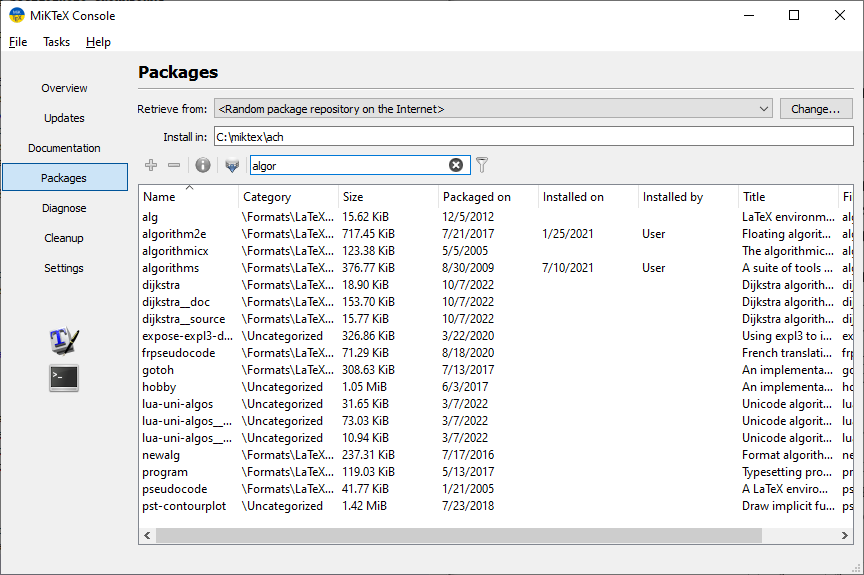
\includegraphics[height=5cm]{workbook-extras/miktex-console}
}\quad
\subfloat[правое изображение] {
   \label{составной рисунок 2}
   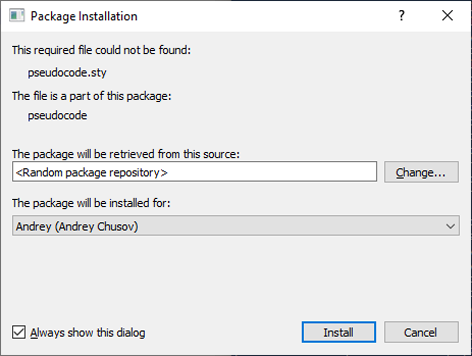
\includegraphics[height=5cm]{
      workbook-extras/miktex-package-installation}
} \\
\subfloat[нижнее изображение]{
   \label{составной рисунок 3}
   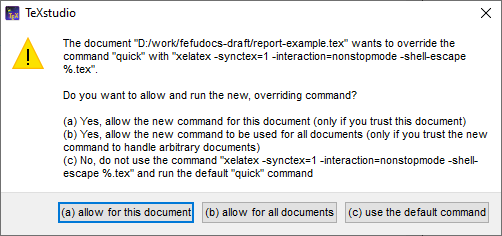
\includegraphics[height=4cm]{
      workbook-extras/texstudio-rules-override}
}
\caption{Пример составного рисунка}
\label{составной рисунок}
\end{figure}

Для этого существует несколько расширений языка \LaTeX{}.
Популярными и удобными являются расширения \texttt{subcaption} и \texttt{subfig}, однако многие издательства журналов Scopus и WebOfScience, такие как Springer, IEEE и ACM, отдают предпочтения второму, а их классы \LaTeX{} являются несовместимыми с расширениями \texttt{subcaption}, поэтому ниже описан метод создания таких составных рисунков, предоставляемый расширением \texttt{subfig}.

Это расширение среди прочего добавляет в список директив, которые можно использовать внутри окружения \texttt{figure}, директиву \verb+\subfloat+, которая в качестве обязательного параметра принимает описание добавляемого в качестве подрисунка изображение, а в качестве опционального --- текст подрисуночной надписи, которая относится к подрисунку.

Например, код, использованный для вставки рисунка \ref{составной рисунок} в документ \LaTeX{}, следующий:
\begin{verbatim}
\begin{figure}[ht]
\centering
\subfloat[левое изображение] {
   \label{составной рисунок 1}
   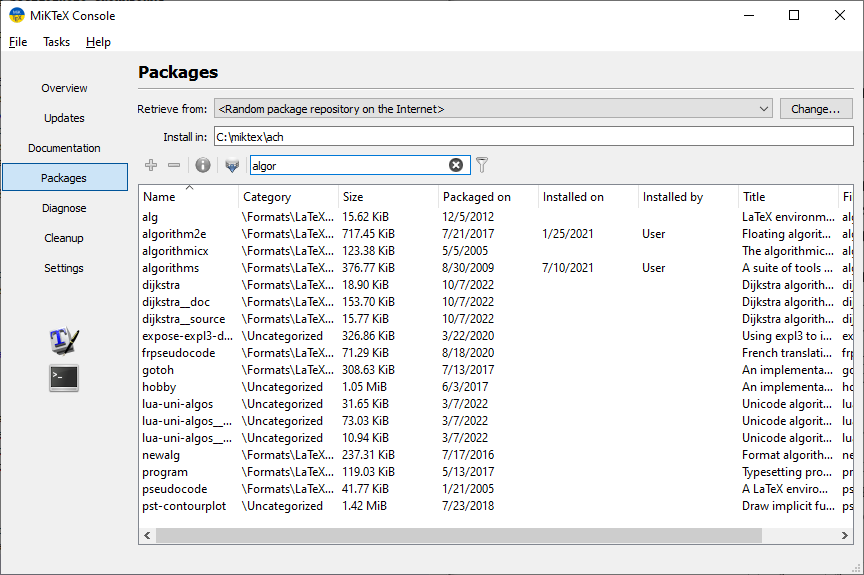
\includegraphics[height=5cm]{workbook-extras/miktex-console}
}\quad
\subfloat[правое изображение] {
   \label{составной рисунок 2}
   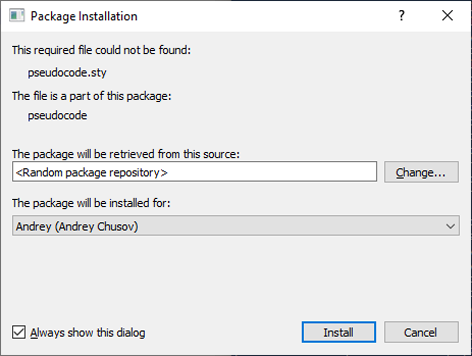
\includegraphics[height=5cm]{
      workbook-extras/miktex-package-installation}
} \\
\subfloat[нижнее изображение]{
   \label{составной рисунок 3}
   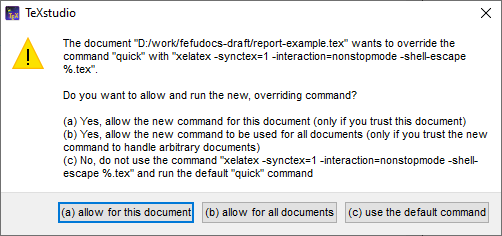
\includegraphics[height=4cm]{
      workbook-extras/texstudio-rules-override}
}
\caption{Пример составного рисунка}
\label{составной рисунок}
\end{figure}
\end{verbatim}

На весь рисунок составной рисунок можно ссылаться, как и в случае с простыми рисунками, используя директиву \verb+\ref+ с текстом \verb+\label+ в качестве параметра.
Например, \verb+\ref{составной рисунок}+ транслируется в номер рисунка \ref{составной рисунок}.

Компоненты рисунка идентифицируются директивой \verb+\label+, которая располагается "внутри" (то есть в обязательном параметре) директивы \verb+\subfigure+.
Например, на правое изображение в приведенном примере можно сослаться, используя команду \verb+\ref{составной рисунок 2}+, что производит ссылку: \ref{составной рисунок 2}.

В коде выше, использованном для добавления рисунка \ref{составной рисунок}, обратите внимание на две директивы.

Директива \verb+\quad+ используется для принудительного добавления пробела в \LaTeX{} даже там, откуда он обычно убирается.
На рисунке \ref{составной рисунок} он использован для добавления некоторого расстояния между рисунками \ref{составной рисунок 1} и \ref{составной рисунок 2}.
Существует чуть более длинная версия принудительного пробела, реализуемая директивой \verb+\qquad+ (с двумя "q").
Такие принудительные пробелы могут быть использованы и в других местах, например в формулах.

Также обратите внимание на то, что рисунок \ref{составной рисунок 3} вынесен в отдельную строку, что сделано с помощью директивы \textbackslash\textbackslash{} принудительного переноса строк (см.~раздел~\ref{подраздел про абзацы}).

\subsubsection{Рисование непосредственно в \LaTeX{}.}\label{раздел про рисование в latex}
Существует несколько инструментов, позволяющих рисовать в документе \LaTeX{}, задавая изображение его текстовым описанием.
Одним из наиболее примитивных является окружение \texttt{picture}, доступное при использовании любых компиляторов и дистрибутивов \LaTeX{}.
Однако его функции сильно ограничены, а его команды не удобны, поскольку в значительной мере опираются на координатную сетку документа и требуют значительной работы с деталями его реализации.

Гораздо более функциональным является язык для описания изображений, предоставляемый расширением \texttt{TikZ} и одноименным языком \cite{tikz-website, tikz-ctan}, дополняющим \LaTeX{}.
Расширение и компиляторы TikZ поставляется в составе большинства современных дистрибутивов \TeX{} и \LaTeX{} вместе с большим количеством собственных расширений и библиотек, подключаемых в преамбуле документа \LaTeX{} с помощью директивы \verb+usetikzlibrary+ во многом подобно директиве \verb+\usepackage+ языка \LaTeX{}.
Список библиотек TikZ обширен и включает в себя такие как
\begin{description}
\item[3d] для рисования в трехмерных координатах (см. также \texttt{perspective});
\item[automata] для рисования автоматов и вычислительных машин с состояниями;
\item[circuits] для рисования принципиальных электрических и логических схем;
\item[er] для рисования ER-диаграмм объект-отношение (entity-relationship);
\item[fadings] для использования градиентов;
\item[lindenmayersystems] для рисования фрактальных структур;
\item[perspective] для трехмерных структур; в отличие от библиотеки \texttt{3d} позволяет строить проекционные, не только изометрические, изображения;
\item[petri] для рисования сетей Петри, которые также как и \texttt{automata} описывают состояния систем, однако имеют более широкий круг применения в системотехнике;
\item[tree] для рисования иерархических и древовидных структур;
\item[angles] для выполнения операций и рисования углов;
\item[arrows] --- библиотека стрелок;
\item[calc] дает б\'{о}льшую гибкость при вычислениях координат и автоматизации рисования;
\item[fpu] позволяет выполнять более точные вычисления на основе арифметики с плавающей запятой;
\item[patterns] для использования в рисунках мозаичных структур (например, штрихование);
\item[shadows] для рисования теней;
\item[shape] библиотека геометрических фигур;
\end{description}
и другие.

Преимуществами TikZ по сравнению с обычными файлами в рисунках являются, во-первых, инкапсуляция рисунков в одном документе и отсутствии необходимости сопровождать файлы \LaTeX{} дополнительными файлами рисунков, а во-вторых, в согласованности размеров и стилей оформления, например размеров и шрифтов текстовых элементов, формул, которые можно задавать, используя тот же синтаксис из раздела \ref{раздел про формулы}, с правилами, которые заданы для документа в целом.

Пример блок-схемы алгоритма на языке TikZ:
\begin{verbatim}
\begin{figure}[ht]
\centering
\begin{tikzpicture}
 [
  every node/.style={
   node distance=0.4cm and 0.3cm
  },
  start/.style={circle, draw},
  end/.style={circle, draw, anchor=south},
  init/.style={
   trapezium, draw, trapezium left angle=60,
   trapezium right angle=120, align=left
  },
  action/.style={rectangle, draw},
  conditional/.style={diamond, shape aspect=2, draw}
 ]
 \node[start] (start) {};
 \node[init, below=of start] (input){
  $x \in F$ --- основание \\
  $y_M\in\mathbb{N}_0$ --- мантисса степени \\
  $y_E \in \mathbb{N}_0$ --- экспонента степени
 };
 \node[action, below=of input] (записать 1 в r)
  {$r \leftarrow 1$};
 \node[action, below=of записать 1 в r] (записать x в t) {
  $t \leftarrow x$
 };
 \node[conditional, below=of записать x в t]
  (проверить y равно 0) {$y_M = 0$};
 \node[conditional, below=of проверить y равно 0]
  (проверить четность y) {$y_M \bmod 1 = 1$};
 \node[action, below right=of проверить четность y]
  (увеличить r) {$r \leftarrow r \cdot t$};
 \node[action, below=of проверить четность y] (увеличить t) {
  $t \leftarrow t \cdot t$
 };
 \node[action, below=of увеличить t] (разделить y на 2) {
  $I_{y_I} \leftarrow \lfloor y_M/2 \rfloor$
 };
 \node[action, right=of проверить y равно 0]
  (учесть экспоненту y) {$r \leftarrow r^{(\beta^{y_E})}$};
 \node[end, right=of учесть экспоненту y] (конец){};
 \node[right=of конец] {вернуть $r$};
 \draw (start) -> (input) -> (записать 1 в r) -> (записать x в t)
  -> (проверить y равно 0) coordinate [midway] (начало цикла)
   -> (проверить четность y) node[at start, right] {\tiny{0}}
    -> (увеличить t) node [at start, right] {\tiny{0}}
     -> (разделить y на 2);
 \coordinate[left=of проверить четность y]
  (точка левее 2-го условия);
 \draw (разделить y на 2) -| (точка левее 2-го условия)
  |- (начало цикла);
 \draw (проверить четность y)
  -| (увеличить r) node[at start, above] {\tiny{1}}
   -| (увеличить t);
 \draw (проверить y равно 0)
  -> (учесть экспоненту y) node [at start, above] {\tiny{1}}
   -> (конец);
\end{tikzpicture}
\caption{Возведение $x$ неотрицательную степень
  $y = y_M \cdot \beta^{y_E}$}
\label{блок-схема алгоритма на tikz}
\end{figure}
\end{verbatim}

Результатом является рисунок \ref{блок-схема алгоритма на tikz}.
\begin{figure}[ht]
\centering
\begin{tikzpicture}
 [
  every node/.style={
   node distance=0.4cm and 0.3cm
  },
  start/.style={circle, draw},
  end/.style={circle, draw, anchor=south},
  init/.style={
   trapezium, draw, trapezium left angle=60,
   trapezium right angle=120, align=left
  },
  action/.style={rectangle, draw},
  conditional/.style={diamond, shape aspect=2, draw}
 ]
 \node[start] (start) {};
 \node[init, below=of start] (input){
  $x \in F$ --- основание \\
  $y_M\in\mathbb{N}_0$ --- мантисса степени \\
  $y_E \in \mathbb{N}_0$ --- экспонента степени
 };
 \node[action, below=of input] (записать 1 в r)
  {$r \leftarrow 1$};
 \node[action, below=of записать 1 в r] (записать x в t) {
  $t \leftarrow x$
 };
 \node[conditional, below=of записать x в t]
  (проверить y равно 0) {$y_M = 0$};
 \node[conditional, below=of проверить y равно 0]
  (проверить четность y) {$y_M \bmod 1 = 1$};
 \node[action, below right=of проверить четность y]
  (увеличить r) {$r \leftarrow r \cdot t$};
 \node[action, below=of проверить четность y] (увеличить t) {
  $t \leftarrow t \cdot t$
 };
 \node[action, below=of увеличить t] (разделить y на 2) {
  $I_{y_I} \leftarrow \lfloor y_M/2 \rfloor$
 };
 \node[action, right=of проверить y равно 0]
  (учесть экспоненту y) {$r \leftarrow r^{(\beta^{y_E})}$};
 \node[end, right=of учесть экспоненту y] (конец){};
 \node[right=of конец] {вернуть $r$};
 \draw (start) -> (input) -> (записать 1 в r) -> (записать x в t)
  -> (проверить y равно 0) coordinate [midway] (начало цикла)
   -> (проверить четность y) node[at start, right] {\tiny{0}}
    -> (увеличить t) node [at start, right] {\tiny{0}}
     -> (разделить y на 2);
 \coordinate[left=of проверить четность y]
  (точка левее 2-го условия);
 \draw (разделить y на 2) -| (точка левее 2-го условия)
  |- (начало цикла);
 \draw (проверить четность y)
  -| (увеличить r) node[at start, above] {\tiny{1}}
   -| (увеличить t);
 \draw (проверить y равно 0)
  -> (учесть экспоненту y) node [at start, above] {\tiny{1}}
   -> (конец);
\end{tikzpicture}
\caption{Возведение $x$ неотрицательную степень
  $y = y_M \cdot \beta^{y_E}$}
\label{блок-схема алгоритма на tikz}
\end{figure}

Примеры графиков функций, описанных на языке TikZ,  приведены на рисунке \ref{sinc в tikz}.
Эти графики получены в результате компиляции следующего кода \LaTeX{}.
\begin{verbatim}
\begin{figure}[ht]
\centering
\subfloat[в декартовых координатах]{
 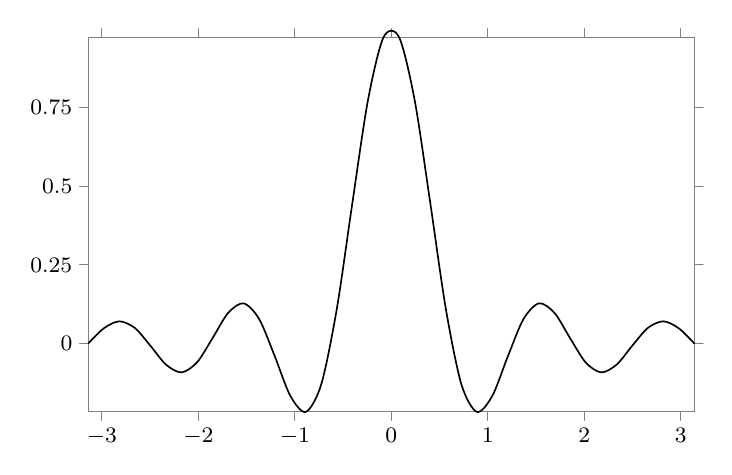
\begin{tikzpicture}[scale=1.54] \datavisualization
  [
   scientific axes,
   visualize as smooth line=sinc
  ]
  data [set=sinc, format=function] {
   var x : interval[-pi:pi] samples 40;
   func y = sin(5*\value x r) /(5*\value x);
  };
 \end{tikzpicture}
}
\quad
\subfloat[в полярных координатах]{
 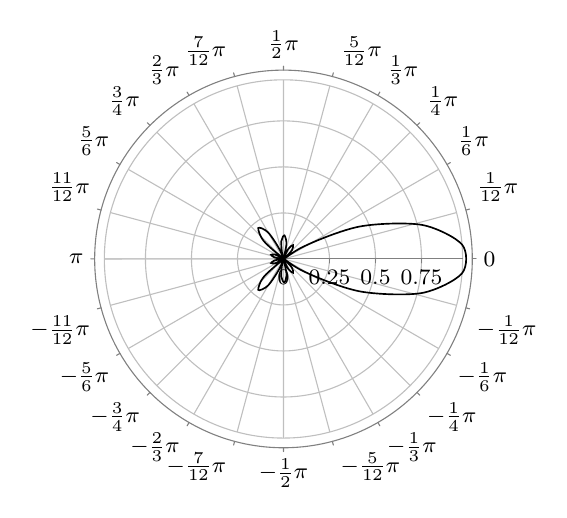
\begin{tikzpicture}[scale=.7] \datavisualization
  [
   scientific polar axes={-pi to pi, clean},
   all axes=grid,
   visualize as smooth line=sinc
  ]
  data [set=sinc, format=function] {
   var angle : interval[-pi:pi] samples 40;
   func radius = sin(5*\value{angle}r) /(5*\value{angle});
  };
 \end{tikzpicture}
}
\caption{Графики функции $\operatorname{sinc} x =
   \frac{\sin x}{x}$}
\label{sinc в tikz}
\end{figure}
\end{verbatim}

\begin{figure}[ht]
\centering
\subfloat[в декартовых координатах]{
 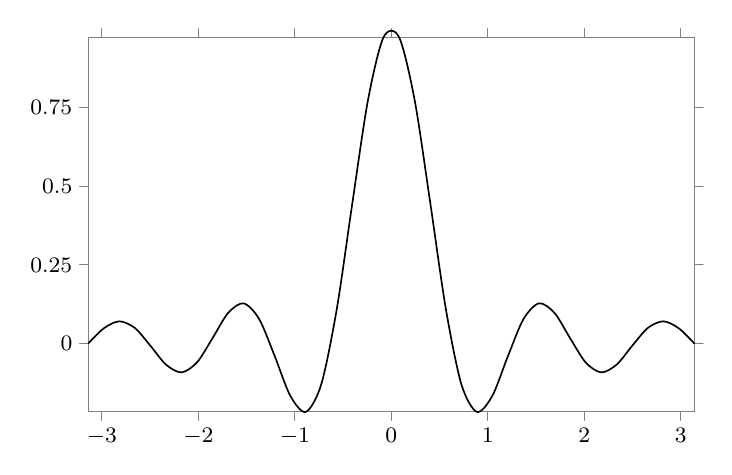
\begin{tikzpicture}[scale=1.54] \datavisualization
  [
   scientific axes,
   visualize as smooth line=sinc
  ]
  data [set=sinc, format=function] {
   var x : interval[-pi:pi] samples 40;
   func y = sin(5*\value x r) /(5*\value x);
  };
 \end{tikzpicture}
}
\quad
\subfloat[в полярных координатах]{
 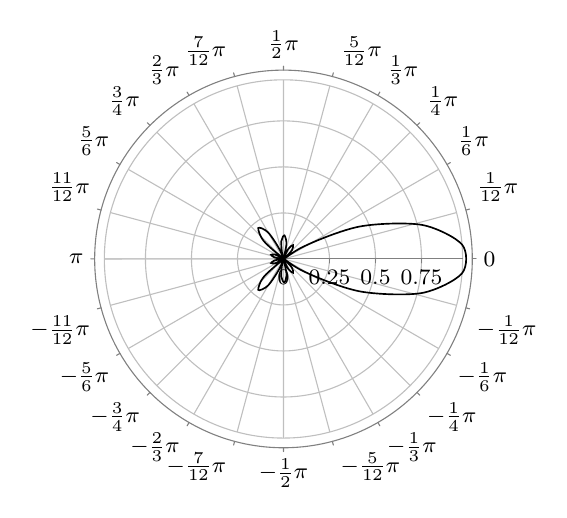
\begin{tikzpicture}[scale=.7] \datavisualization
  [
   scientific polar axes={-pi to pi, clean},
   all axes=grid,
   visualize as smooth line=sinc
  ]
  data [set=sinc, format=function] {
   var angle : interval[-pi:pi] samples 40;
   func radius = sin(5*\value{angle}r) /(5*\value{angle});
  };
 \end{tikzpicture}
}
\caption{Графики функции $\operatorname{sinc} x =
   \frac{\sin x}{x}$}
\label{sinc в tikz}
\end{figure}

Описание TikZ и более низкоуровневого языка PGF, на который опираются компиляторы TikZ, выходит за рамки задач данного документа, однако хорошие учебные и справочные материалы доступны на официальном сайте TikZ \cite{tikz-website}.

\subsection{Таблицы}
Набор таблиц в \LaTeX{} возможно оказываются наименее удобным из всех инструментов.
Поэтому в Интернет \cite{tablesgenerator} и в средах разработки (рис. \ref{таблицы TeXstudio}) доступны средства для визуального создания таблиц, однако эти средства ограничены только стандартными таблицами и чаще не поддерживают дополнительных средств, предоставляемых расширениями.
\begin{figure}[ht]
\centering
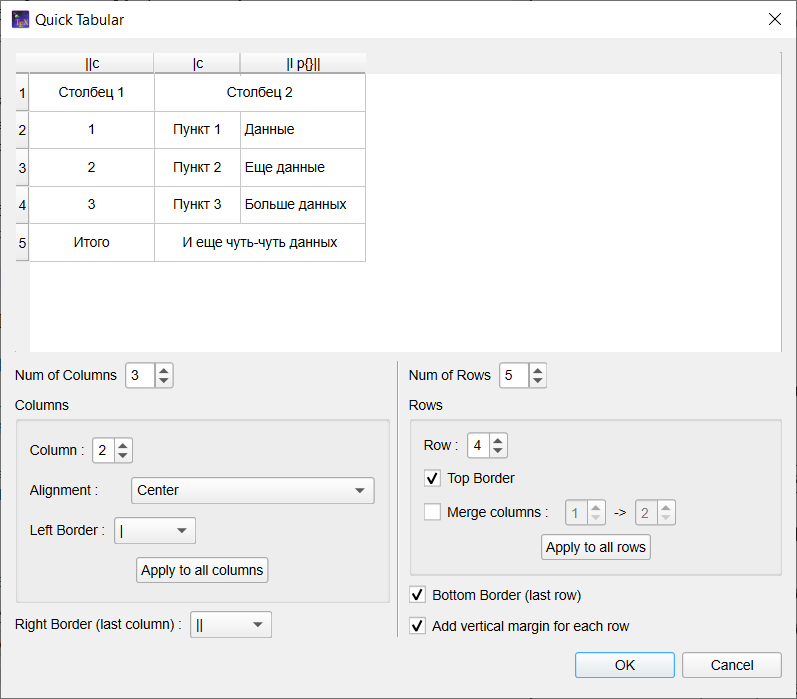
\includegraphics[width=7cm]{workbook-extras/texstudio-tables}
\caption{Визуальное создание таблиц в TeXstudio}
\label{таблицы TeXstudio}
\end{figure}
В данном разделе описаны методы ручного описания таблиц в исходном тексте \LaTeX{}.

Как и в случае с рисунками таблицы задаются, во-первых, описанием содержания таблицы и её структуры, а во-вторых --- позицией плавающих таблиц в окружающем тексте, их заголовками и идентификаторами.

\subsubsection{Синтаксис описания содержимого таблицы.}\label{подраздел про набор содержимого таблицы}
Синтаксис для описания таблиц во многом схож с описанием матриц в формулах, поскольку, также как и для описания матриц, для разграничения строк используется директива \textbackslash\textbackslash{} принудительного разрыва строк, а для разграничения столбцов --- символ амперсанда "\&".

Стандартные таблицы строятся в окружении \texttt{tabular} и, в отличие от матриц, принимают в качестве параметра методы выравнивания и рисования границ для каждого столбца индивидуально, как указано в таблице \ref{таблица с параметрами tabular}.
\begin{table}[ht]
\centering
\caption{Позиционные параметры таблицы \texttt{tabular}}
\label{таблица с параметрами tabular}
\begin{tabular}{|c|p{10cm}|}
\hline \texttt{l} & Задает выравнивание по левому краю столбца. \\
\hline \texttt{c} & Задает выравнивание по середине столбца. \\
\hline \texttt{r} & Задает выравнивание по правому краю столбца. \\
\hline \texttt{p\{ширина\}} & Задает столбец типа "параграф". Текст в ячейках такого столбца автоматически переносится в соответствии с с заданной в фигурных скобках шириной. Данный столбец настоящей таблицы имеет тип \texttt{p}. \\
\hline \texttt{m\{ширина\}} & Тоже задает столбец типа "параграф", но вертикальная середина текста в ячейках столбца выравнивается с верхней границей текста в соседних столбцах типов \texttt{l}, \texttt{c} или \texttt{r}. \\
\hline \texttt{b\{ширина\}} & Тоже столбец типа "параграф", но в отличие от остальных случаев, нижний край текста выравнивается с верхними границами столбцов \texttt{l}, \texttt{c} и \texttt{r}, а также с вертикальной серединой текста в столбцах типа \texttt{m}. \\
\hline
\end{tabular}
\end{table}

Кроме выравнивания между и вокруг столбцов также могут быть заданы визуальные границы: одинарные (с помощью вертикальной черты "|") или двойные (с помощью двух вертикальных черт "||").

В каждой строке такой таблицы может быть также задана директива \verb+\hline+, которая приводит к тому, что над \textit{всей} строкой такой таблицы рисуется горизонтальная линия.
Поэтому для рисования завершающей, нижней, границы таблицы требуется создание дополнительной строки с единственной директивой \verb+\hline+ в ней.
Для рисования двойной горизонтальной границы используется директива \verb+\hhline+ из расширения \texttt{hhline} языка \LaTeX{}.

Пример простейшей таблицы:
\begin{verbatim}
\begin{tabular}{l|rc}
\textbf{ФИО}         & \textbf{Группа}      & \textbf{Телефон} \\
\hline
Иванов Иван Иванович & М3122-11.04.02срр    & +7 222 333 44 55 \\
Петров Петр Петрович & Б9120-09.03.04прогин & +7 666 777 88 99 \\
Сидов  Сид  Сидович  & М9123-09.04.04рпис   & +7 000 111 22 33 \\
\hline
\end{tabular}
\end{verbatim}
Этот код компилируется в таблицу \\
\begin{tabular}{l|rc}
\textbf{ФИО}            & \textbf{Группа}      & \textbf{Телефон} \\
\hline
Иванов Иван Иванович & М3122-11.04.02срр    & +7 222 333 44 55 \\
Петров Петр Петрович & Б9120-09.03.04прогин & +7 666 777 88 99 \\
Сидов  Сид  Сидович  & М9123-09.04.04рпис   & +7 000 111 22 33 \\
\hline
\end{tabular}

Обратите внимание на указанные типы столбцов: \texttt{l|rc}.
В соответствии с такой спецификацией, во-первых, левый столбец не содержит со своей левой стороны рисуемой границы, а его содержимое выравнивается по левому (l --- "\underline{l}eft") краю; во-вторых, между первым и вторым столбцами вертикальной чертой задано рисование одинарной вертикальной границы; в-третьих, текст второго столбца выравнивается по правому (r --- "\underline{r}ight") краю этого столбца; в-четвертых между вторым и третьим столбцами граница не рисуется; в-пятых, в третьем, правом, столбце текст выравнивается центру (c --- "\underline{c}enter"); в-шестых, правый столбец справа не содержит рисуемой границы.

Также обратите внимание на рисуемые горизонтальные границы и их соответствие директиве \verb+\hline+ в коде \LaTeX{} для этой таблицы.

Ниже представлен пример таблицы с параграфами (то есть многострочным содержимым ячеек столбца).
Обратите также внимание на использование двойных границ --- вертикальных слева и справа в соответствии со спецификацией, в которой эти границы заданы по краям двумя сплошными вертикальными линиями.
Также в этом же примере использовано расширение \texttt{hhline} и одноимённой директивы \verb+\hhline+, описание которой не приводится здесь, но его очень короткая документация на английском языке приведена в \cite{hhline}.
\begin{verbatim}
\begin{tabular}{||l|p{4cm}|m{4cm}|b{4cm}||}
\hhline{|t:====:t|}
1. & Параграф \texttt{p}, который выравнивается
     по верхней границе текста.
   & Параграф \texttt{m} с равнением текста по вертикальной
     середине.
   & Параграф \texttt{b} с равнением по нижней границе. \\
\hline
2. & Это следующий параграф \texttt{p}, который выравнивается по
     верхней границе текста.
   & Еще один параграф типа \texttt{m}, текст которого
     выравнивается по своей середине с текстом других ячеек той
     же строки.
   & Еще один параграф \texttt{b} с вырвниванием текста по его
     низу. \\
\hhline{|b:====:b|}
\end{tabular}
\end{verbatim}
Указанный код собирается в таблицу\\
\begin{tabular}{||l|p{4cm}|m{4cm}|b{4cm}||}
\hhline{|t:====:t|}
1. & Параграф \texttt{p}, который выравнивается
     по верхней границе текста.
   & Параграф \texttt{m} с равнением текста по вертикальной
     середине.
   & Параграф \texttt{b} с равнением по нижней границе. \\
\hline
2. & Это следующий параграф \texttt{p}, который выравнивается по
     верхней границе текста.
   & Еще один параграф типа \texttt{m}, текст которого
     выравнивается по своей середине с текстом других ячеек той
     же строки.
   & Еще один параграф \texttt{b} с вырвниванием текста по его
     низу. \\
\hhline{|b:====:b|}
\end{tabular}

Обращаем внимание на то, что, как и в случае с матрицами в формулах, выравнивания текста в исходном тексте \LaTeX{}, как это сделано выше, не требуется для корректного отображения таблицы, но оно удобно для визуального восприятия исходного текста и сопровождения таблиц и исправления ошибок.

Также как и в случае с рисунками (директивой \verb+\includegraphics+ --- см. раздел~\ref{раздел про рисунки из файла}) для выравнивания таких таблиц по центру может быть использовано окружение \texttt{center}, например
\begin{verbatim}
\begin{center}
\begin{tabular}{l|lc}
\textbf{ФИО}         & \textbf{Группа}      & \textbf{Телефон} \\
\hline
Иванов Иван Иванович & М3122-11.04.02срр    & +7 222 333 44 55 \\
Петров Петр Петрович & Б9120-09.03.04прогин & +7 666 777 88 99
\end{tabular}
\end{center}
\end{verbatim}
что производит \\
\begin{center}
\begin{tabular}{l|lc}
\textbf{ФИО}         & \textbf{Группа}      & \textbf{Телефон} \\
\hline
Иванов Иван Иванович & М3122-11.04.02срр    & +7 222 333 44 55 \\
Петров Петр Петрович & Б9120-09.03.04прогин & +7 666 777 88 99
\end{tabular}
\end{center}

Для объединения нескольких горизонтально расположенных ячеек таблицы в один служит директива \verb+\multicolumn+, которая принимает три обязательных параметра --- число объединяемых столбцов, способ оформления текста в объединенной ячейке и содержимое объединённой ячейки.

Для объединения нескольких вертикально расположенных ячеек таблицы служит директива \verb+\multirow+, использование которой однако, в отличие от \verb+\multicolumn+, требует подключения расширения \texttt{multirow}.
Также как и \verb+\multicolumn+, директива \verb+\multirow+ принимает три обязательных параметра, но в отличие от \verb+\multicolumn+, второй параметр задает ширину объединенной ячейки и допускает указание астериска "*" для вычисления содержимого на основе содержания ячейки.

Независимо от того, как объединены строки ячейки, рассмотренная выше директива \verb+\hline+ рисует горизонтальную линию через \textit{всю таблицу}, даже если эта линия будет пересекать текст объединённой ячейки.
Во избежание этого используется директива \verb+\cline+, которая принимает в качестве параметра диапазон столбцов, через который она должна проходить, например \verb+\cline{2-4}+.
Данную директиву можно указывать несколько раз, например \verb+\cline{2-4}\cline{6-6}+.

Пример \LaTeX{}-кода таблицы с объединенными ячейками:
\begin{verbatim}
\begin{tabular}{|r|l|c|c|}
\hline
\multirow{2}{*}{№}&\multicolumn{2}{c|}{Студенты}&\multirow{2}{*}
                                                  {Подгруппа} \\
\cline{2-3}       & ФИО            &     Оценка &             \\
\hline          1 & Андреев Б. В.  &          1 &\multirow{3}
                                                       {*}{I} \\
\cline{1-3}     2 & Борисов Г. В.  &          2 &             \\
\cline{1-3}     3 & Викторов Г. Д. &          3 &             \\
\hline          4 & Григорьев Д. В &          4 & \multirow{2}
                                                       {*}{II}\\
\cline{1-3}     5 & Дмитриев Е. Ж. &          5 &             \\
\hline
\end{tabular}
\end{verbatim}
В результате трансляции таблица приобретает вид \\
\begin{tabular}{|r|l|c|c|}
\hline
\multirow{2}{*}{№} & \multicolumn{2}{c|}{Студенты}& \multirow{2}{*}
                                                    {Подгруппа} \\
\cline{2-3}        & ФИО             &     Оценка &             \\
\hline           1 & Андреев Б. В.   &          1 & \multirow{3}
                                                         {*}{I} \\
\cline{1-3}      2 & Борисов Г. В.   &          2 &             \\
\cline{1-3}      3 & Викторов Г. Д.  &          3 &             \\
\hline           4 & Григорьев Д. В. &          4 & \multirow{2}
                                                         {*}{II}\\
\cline{1-3}      5 & Дмитриев Е. Ж.  &          5 &             \\
\hline
\end{tabular}

Размеры таблиц, создаваемых с помощью окружения \texttt{tabular}, определяется содержимым их ячеек, а в случае параграфических ячеек типов \texttt{p}, \texttt{m} и \texttt{b} ещё и требуют ручного задания ширины столбцов.

Это не всегда удобно и не всегда применимо при рисовании таблиц --- иногда требуется задать ширину таблицы целиком и определять ширину индивидуальных столбцов уже на основе этой совокупной ширины.

Для этих целей существуют расширение \texttt{tabularx} языка \LaTeX{} и предоставляемое им одноимённое окружение \texttt{tabularx}, а также расширение \texttt{tabulary} с одноименным окружением \texttt{tabulary}.
Окружение \texttt{tabularx} в наибольшей степени похоже на стандартное окружение \texttt{tabularx}, поэтому ниже рассмотрено оно, а с \texttt{tabulary}, как и со всеми другими расширениями, можно ознакомиться в CTAN \cite{tabulary}.

В отличие от \texttt{tabular}, окружение \texttt{tabularx}, во-первых, требует указания еще одного обязательного параметра --- ширины таблицы, а во-вторых --- предоставляет еще один тип столбца: \texttt{X} в дополнение к указанным в таблице \ref{таблица с параметрами tabular}.
Столбцы типа \texttt{X} определяют столбцы с параграфами, то есть с автоматически переносимым на новые строки длинным текстом подобно стандартному расширению \texttt{p}.
В отличие от столбцов типа \texttt{p}, столбцы типа \texttt{X} имеют вариативную длину --- процессор окружения \texttt{tabularx} может самостоятельно и автоматически подбирать ширину столбцов \texttt{X} на основе, во-первых, ширины таблицы в целом, а во-вторых --- содержимого ячеек столбца.

Например, чтобы растянуть таблицу \ref{таблица с параметрами tabular} на всю страницу, можно использовать следующий код.
\begin{verbatim}
\begin{tabularx}{\textwidth}{|l|X|}
\hline \texttt{l} & Задает выравнивание по левому краю столбца.\\
\hline \texttt{c} & Задает выравнивание по середине столбца. \\
\hline \texttt{r} & Задает выравнивание по правому краю
                                                      столбца. \\
\hline \texttt{p\{ширина\}}
                  & Задает столбец типа "параграф". Текст в
		    ячейках такого столбца автоматически
		    переносится в соответствии с заданной в
		    фигурных скобках шириной. Данный столбец
		    настоящей таблицы имеет тип \texttt{p}. \\
\hline \texttt{m\{ширина\}}
                  & Тоже задает столбец типа "параграф", но
                    вертикальная середина текста в ячейках
		    столбца выравнивается с верхней границей
		    текста в соседних столбцах типов \texttt{l},
		    \texttt{c} или \texttt{r}. \\
\hline \texttt{b\{ширина\}}
                  & Тоже столбец типа "параграф", но в отличие
		    от остальных случаев, нижний край текста
                    выравнивается с верхними границами столбцов
                    \texttt{l}, \texttt{c} и \texttt{r}, а также
		    с вертикальной серединой текста в столбцах
		    типа \texttt{m}. \\
\hline
\end{tabularx}
\end{verbatim}

И этот код производит следующую таблицу: \\
\begin{tabularx}{\textwidth}{|l|X|}
\hline \texttt{l} & Задает выравнивание по левому краю столбца.\\
\hline \texttt{c} & Задает выравнивание по середине столбца. \\
\hline \texttt{r} & Задает выравнивание по правому краю
                                                      столбца. \\
\hline \texttt{p\{ширина\}}
                  & Задает столбец типа "параграф". Текст в
		    ячейках такого столбца автоматически
		    переносится в соответствии с заданной в
		    фигурных скобках шириной. Данный столбец
		    настоящей таблицы имеет тип \texttt{p}. \\
\hline \texttt{m\{ширина\}}
                  & Тоже задает столбец типа "параграф", но
                    вертикальная середина текста в ячейках
		    столбца выравнивается с верхней границей
		    текста в соседних столбцах типов \texttt{l},
		    \texttt{c} или \texttt{r}. \\
\hline \texttt{b\{ширина\}}
                  & Тоже столбец типа "параграф", но в отличие
		    от остальных случаев, нижний край текста
                    выравнивается с верхними границами столбцов
                    \texttt{l}, \texttt{c} и \texttt{r}, а также
		    с вертикальной серединой текста в столбцах
		    типа \texttt{m}. \\
\hline
\end{tabularx}

Также обращаем внимание на расширение \texttt{makecell} \cite{makecell}, которое предоставляет набор директив для кастомизации отображения индивидуальных ячеек таблиц.
Например, ячейка-заголовок может быть указана директивой \verb+\thead+, которая принимает в качестве параметра текст ячейки, и, в отличие от рассмотренных ранее методов включения текста, позволяет, во-первых, настроить единые правила оформления заголовочных ячеек, а во-вторых --- произвольно переносить текст на новые строки с помощью директивы \textbackslash\textbackslash, даже в ячейках типов \texttt{l}, \texttt{c} или \texttt{r}, преобразуя их в многострочные ячейки.
Обычные, не заголовочные, ячейки могут быть аналогичным образом кастомизированы с помощью директивы \verb+\makecell+.

\subsubsection{Плавающие таблицы.}\label{плавающие таблицы}
Как и в случае с рисунками таблицы обычно принято не просто вставлять в текст, но сопровождать их заголовками и номерами, ссылаться на них в тексте, располагая вблизи первой ссылки на них, не делая их частью основного текста документа, как в примерах предыдущего раздела, но формируя \textit{плавающие блоки} в документе подобно рисункам.

Как указано в разделе \ref{плавающие рисунки}, для того, чтобы сделать рисунки плавающими блоками, используется окружение \texttt{figure}, и это окружение на самом деле можно использовать и для таблиц --- но тогда они будут оформлены и пронумерованы как рисунки:
\begin{verbatim}
\begin{figure}[ht]
\centering
\begin{tabular}{l|lc}
\textbf{ФИО}         & \textbf{Группа}      & \textbf{Телефон} \\
\hline
Иванов Иван Иванович & М3122-11.04.02срр    & +7 222 333 44 55 \\
Петров Петр Петрович & Б9120-09.03.04прогин & +7 666 777 88 99
\end{tabular}
\label{таблица как рисунок}
\caption{Таблица, вставленная как рисунок}
\end{figure}
\end{verbatim}
производит таблицу, представленную как рис.~\ref{таблица как рисунок}.
\begin{figure}[ht]
\centering
\begin{tabular}{l|lc}
\textbf{ФИО}            & \textbf{Группа}      & \textbf{Телефон} \\
\hline
Иванов Иван Иванович & М3122-11.04.02срр    & +7 222 333 44 55 \\
Петров Петр Петрович & Б9120-09.03.04прогин & +7 666 777 88 99
\end{tabular}
\caption{Таблица, вставленная как рисунок}
\label{таблица как рисунок}
\end{figure}

Обычно же оформление таблиц требует обращение с ними именно как с таблицами, а не как с рисунками.
Поэтому для этих целей существует отдельное окружение \texttt{table}.
Наполнение окружения \texttt{table} во многом аналогично наполнению окружения \texttt{figure}, и отличается лишь собственной нумерацией и наименованием (например, в зависимости от класса и языка документа, будет отображено слово "таблица" вместо "рисунок").

В действительности и рисунок можно вставить в документ как таблицу:
\begin{verbatim}
\begin{table}[ht]
\centering
\caption{Рисунок, вставленный как таблица}
\label{рисунок как таблица}

\includegraphics[height=2cm]{это рисунок}
\end{table}
\end{verbatim}
что производит "таблицу" \ref{рисунок как таблица}.
\begin{table}[ht]
\centering
\caption{Рисунок, вставленный как таблица}
\label{рисунок как таблица}

\includegraphics[height=2cm]{это рисунок}
\end{table}

В этой связи директивы окружения \texttt{table} эквивалентны директивам окружения \texttt{figure}.
Повторим их кратко:
\begin{itemize}
\item \verb+\centering+ центрирует наполнение своего плавающего блока, заданное ниже директивы;
\item \verb+\caption+ задаёт название плавающего блока, отображаемое в скомпилированном документе;
\item \verb+\label+ задаёт идентификатор плавающего блока, используемый для конструкции ссылок на блок с помощью директивы \verb+\ref+, подобно идентификаторам разделов, рисунков и уравнений, задаваемых этой же директивой.
\end{itemize}
Напомним, что для того, чтобы центрировать таблицу, её описание (например, с помощью окружений \texttt{tabular} или \texttt{tabularx}) должно быть приведено после директивы \verb+\centering+.

В большинстве случаев заголовки таблиц требуется указывать сверху таблиц, а не снизу, как в случае с рисунками, поэтому, в отличие от рисунков, директиву \verb+\caption+ следует указывать до, а не после, описания таблицы.

Как и в случае с рисунками нумерация формируется директивой \verb+\caption+, а не \verb+\label+, поэтому для корректного формирования идентификаторов и ссылок директиву \verb+\label+ следует указывать после директивы \verb+\caption+.

Также как и \texttt{figure} окружение \texttt{table} опционально может принимать позиционные параметры в квадратных скобках: \texttt{h} ("\underline{h}ere"), \texttt{t} ("\underline{t}op"), \texttt{b} ("\underline{b}ottom"), \texttt{p} ("\underline{p}age") и дополнительно предоставляемый расширением \texttt{float} параметр \texttt{H} ("\underline{H}ere"). Подробное описание этих параметров приведено в таблице~\ref{таблица позиционных параметров figure}.
Также как и в случае с \texttt{figure} эффект от этих параметров может быть усилен с помощью восклицательного знака.

Пример, оформленный как плавающий блок и полученной в результате компиляции кода
\begin{verbatim}
\begin{table}[h!t]
\centering
\caption{Таблица как плавающий блок}
\label{плавающая таблица}
\begin{tabular}{|r|l|c|c|}
\hline
\multirow{2}{*}{№}&\multicolumn{2}{c|}{Студенты}&\multirow{2}{*}
                                                  {Подгруппа} \\
\cline{2-3}       & ФИО            &     Оценка &             \\
\hline          1 & Андреев Б. В.  &          1 & \multirow{3}
                                                       {*}{I} \\
\cline{1-3}     2 & Борисов Г. В.  &          2 &             \\
\cline{1-3}     3 & Викторов Г. Д. &          3 &             \\
\hline          4 & Григорьев Д. В.&          4 & \multirow{2}
                                                       {*}{II}\\
\cline{1-3}     5 & Дмитриев Е. Ж. &          5 &             \\
\hline
\end{tabular}
\end{table}
\end{verbatim}
представлен таблицей \ref{плавающая таблица}.
\begin{table}[h!t]
\centering
\caption{Таблица как плавающий блок}
\label{плавающая таблица}
\begin{tabular}{|r|l|c|c|}
\hline
\multirow{2}{*}{№}&\multicolumn{2}{c|}{Студенты}&\multirow{2}{*}
                                                  {Подгруппа} \\
\cline{2-3}       & ФИО            &     Оценка &             \\
\hline          1 & Андреев Б. В.  &          1 & \multirow{3}
                                                       {*}{I} \\
\cline{1-3}     2 & Борисов Г. В.  &          2 &             \\
\cline{1-3}     3 & Викторов Г. Д. &          3 &             \\
\hline          4 & Григорьев Д. В.&          4 & \multirow{2}
                                                       {*}{II}\\
\cline{1-3}     5 & Дмитриев Е. Ж. &          5 &             \\
\hline
\end{tabular}
\end{table}

Расположение заголовка таблицы \ref{плавающая таблица}, ширина которой меньше ширины документа, может быть неудовлетворительным.
Чтобы выравнить заголовок с левым краем таблицы, может быть использовано расширение \texttt{threeparttable} и его одноимённое окружение \texttt{threeparttable}, которое располагается внутри окружения \texttt{table}.
Тогда заголовок \verb+\caption+, идентификатор \verb+\label+ и содержимое таблицы, в свою очередь, указывается внутри окружения \texttt{threeparttable}.

Таким образом код таблицы \ref{плавающая таблица} можно модифицировать:
\begin{verbatim}
\begin{table}[h!t]
\centering
\begin{threeparttable}
\caption{Таблица как плавающий блок с выравненным заголовком}
\label{плавающая таблица с выравненным заголовком}
\begin{tabular}{|r|l|c|c|}
\hline
\multirow{2}{*}{№}&\multicolumn{2}{c|}{Студенты}& \multirow{2}
                                               {*}{Подгруппа} \\
\cline{2-3}       & ФИО             &    Оценка &             \\
\hline          1 & Андреев Б. В.   &         1 & \multirow{3}
                                                       {*}{I} \\
\cline{1-3}     2 & Борисов Г. В.   &         2 &             \\
\cline{1-3}     3 & Викторов Г. Д.  &         3 &             \\
\hline          4 & Григорьев Д. В. &         4 & \multirow{2}
                                                       {*}{II}\\
\cline{1-3}     5 & Дмитриев Е. Ж.  &         5 &             \\
\hline
\end{tabular}
\end{threeparttable}
\end{table}
\end{verbatim}
и получить таблицу \ref{плавающая таблица с выравненным заголовком} с выравненным заголовком.
\begin{table}[h!t]
\centering
\begin{threeparttable}
\caption{Таблица как плавающий блок с выравненным заголовком}
\label{плавающая таблица с выравненным заголовком}
\begin{tabular}{|r|l|c|c|}
\hline
\multirow{2}{*}{№}&\multicolumn{2}{c|}{Студенты}& \multirow{2}
                                               {*}{Подгруппа} \\
\cline{2-3}       & ФИО             &    Оценка &             \\
\hline          1 & Андреев Б. В.   &         1 & \multirow{3}
                                                       {*}{I} \\
\cline{1-3}     2 & Борисов Г. В.   &         2 &             \\
\cline{1-3}     3 & Викторов Г. Д.  &         3 &             \\
\hline          4 & Григорьев Д. В. &         4 & \multirow{2}
                                                       {*}{II}\\
\cline{1-3}     5 & Дмитриев Е. Ж.  &         5 &             \\
\hline
\end{tabular}
\end{threeparttable}
\end{table}

\subsubsection{Многостраничные таблицы.}
Иногда требуется создавать крупные таблицы, которые вследствие своего размера растягиваются на несколько страниц.
Хотя таких ситуаций следует избегать, если альтернатив нет, то можно использовать расширение \texttt{longtable} \cite{longtable}, которое предоставляет одноимённое окружение \texttt{longtable}, сразу заменяющее собой стандартные окружения \texttt{table} и \texttt{tabular}.
Примером многостраничной таблицы является таблица \ref{таблица с методами выделения текста}.

Для разграничения директив, относящихся к определению плавающего блока \texttt{longtable}, и директив, которые относятся непосредственно к определению содержимого таблицы, служат директивы \verb+\endfirsthead+, \verb+\endhead+, \verb+\endfoot+ и \verb+\endlastfoot+.

Основной заголовок всей таблицы, отображаемый на первой странице, на которой отображается таблица в результате компиляции и задаваемый с помощью известной директивы \verb+\caption+, а также идентификатор таблицы, задаваемый с помощью директивы \verb+\label+, указываются в самом начале, сразу за возможным \verb+\centering+, окружения \texttt{longtable}.
После этого необходимо указать, что описание таблицы для её первой страницы завершено с помощью директивы \verb+\endfirsthead+.
Заголовки этой же таблицы, отображаемые на последующих страницах, указываются с помощью той же директивы \verb+\caption+ между \verb+\endfirsthead+ и \verb+\endhead+.
Если заголовок требуется указать только на первой странице, обе директивы --- \verb+\endfirsthead+ и \verb+\endhead+ указываются одна за другой.

После директивы \verb+\endhead+ может задаваться содержимое многостраничной таблицы.

Ниже приведен фрагмент длинной таблицы из рабочей учебной программы университета, растянутой на несколько таблиц.
Для того, чтобы установить заголовки, используется директива \verb+\thead+ из расширения \texttt{makecell}, упомянутого в разделе \ref{подраздел про набор содержимого таблицы}.
Также обращаем внимание на размер текста в таблице, который установлен в соответствии с нормативами университета.
Это сделано, во-первых, для заголовков --- переопределением директивы \verb+\theadfont+ расширения \texttt{makecell}, переопределения директив в \LaTeX{} выполняются с помощью директивы \verb+\renewcommand+, описание которой выходит за рамки данного документа, поскольку в общем случае это требует рассмотрения аспектов программирования на Тьюринг-полных языках \TeX{} и \LaTeX{}.

Во-вторых, малый размер шрифта для таблицы установлен директивой-переключателем \verb+\footnotesize+ (этот размер в рефератах класса \texttt+fefudoc+ соответствует требуемому).
Как указано в разделе \ref{раздел про директивы}, такие директивы действуют до выхода из структурного компонента текста \LaTeX{} (то есть до закрывающей фигурной скобки, если переключение произошло внутри таких скобок), либо до явного или опосредованного (например директивой нового раздела) использования альтернативной директивы.

Поэтому, чтобы размер текста был изменен только для таблицы и ничего более, после окончания описания длинной таблицы выполняются два действия: восстанавливается исходный стиль отображения заголовков \verb+\thead+, используя ту же директиву \verb+\theadfont+, а также восстанавливается нормальный размер документа использованием директивы переключателя \verb+\normalsize+.

Код длинной таблицы следующий.
\begin{verbatim}
\renewcommand\theadfont{\footnotesize\bfseries}
\footnotesize
\begin{longtable}{|l|p{3cm}|p{2.5cm}|p{3.2cm}|p{2.2cm}|p{2.3cm}|}
\caption{Пример длинной таблицы}\label{длинная таблица}
\endfirsthead
\caption{Пример длинной таблицы (\textit{продолжение})}
\endhead
\hline
\multirow{3}{*}{\thead[l]{№\\п/п}} &
\multirow{4}{*}
 {\thead[l]{Контролируемые\\модули/разделы/\\темы дисциплины}} &
\multirow{5}{*}
 {\thead[l]{Код\\идентификатора\\достижения\\компетенции}} &
\multirow{2}{*}{\thead[l]{Результаты обучения}} &
\multicolumn{2}{c|}{\thead[l]
 {Оценочные средства --- \\ наименование}} \\
\cline{5-6}                           &
                                      &
                                      &
                                      &
\thead[l]{текущий\\контроль}          &
\thead[l]{промежуточная\\аттестация} \\
\hline
1 & Методология автоматизированного проектирования
  & ОПК-1.1 Систематизирует положения, законы и методы в области
    математики, естественных и технических наук для решения задач
    управления
  & Знает актуальные методы автоматизированного
    проектирования технических систем и фундаментальных принципов
    автоматизированного проектирования.
  & Собеседование (УО-1); дискуссия (УО-4); конспект (ПР-7).
  & Вопросы к зачету 1, 4, 7, 10. \\
\cline{4-6}
  &
  &
  & Умеет применять методы автоматизированного проектирования
    технических систем, формулировать и обосновывать адекватные
    требования к системам автоматизированного проектирования.
  & Собеседование (УО-1); дискуссия (УО-4); конспект (ПР-7).
  & Вопросы к зачету 1, 4, 7, 10. \\
\cline{4-6}
  &
  &
  & Владеет навыками использования методов проектирования,
    моделирования и анализа технических систем с помощью систем
    автоматизированного проектирования.
  & Собеседование (УО-1); дискуссия (УО-4); конспект (ПР-7).
  & Вопросы к зачету 1, 4, 7, 10. \\
\cline{3-6}
  &
  & ОПК-1.2 Выявляет сущность проблем управления
  & Знает методы компьютерной реализации систем
    автоматизированного проектирования, принципов
    использования распространенных систем компьютерного
    проектирования и моделирования технических систем.
  & Собеседование (УО-1); дискуссия (УО-4); конспект (ПР-7).
  & Вопросы к зачету 2, 5, 8. \\
\cline{4-6}
  &
  &
  & Умеет самостоятельно решать задачи проектирования,
    моделирования, синтеза и анализа компьютерных моделей
    технических систем, выбирать и развертывать адекватные
    компоненты комплекса средств компьютерного
    автоматизированного проектирования и приводить формальное
    обоснование принятых решений документально.
  & Собеседование (УО-1); дискуссия (УО-4); конспект (ПР-7).
  & Вопросы к зачету 2, 5, 8. \\
\cline{4-6}
  &
  &
  & Владеет навыками решения задач профессиональной
    деятельности, проектирования, моделирования и анализа
    технических систем и устройств, с помощью средств
    компьютерного автоматизированного проектирования.
  & Собеседование (УО-1); дискуссия (УО-4); конспект (ПР-7).
  & Вопросы к зачету 2, 5, 8. \\
\hline
\end{longtable}
\renewcommand\theadfont{\normalsize\bfseries}
\normalsize
\end{verbatim}

Обратите внимание на наличие двух заголовков, директив \verb+\caption+, внутри окружения \texttt{longtable}.
Первый и главный из них, указываемый до директивы \verb+\endfirsthead+, отображается только на первой странице, на которой отображена таблица.
Второй указан после \verb+\endfirsthead+ и до \verb+\endhead+; он отображается только на дополнительных страницах, на которых оказывается таблица.
Этот второй заголовок можно не указывать (то есть удалить в примере второе использование директивы \verb+\caption+), что приведет к тому, что в результате компиляции на дополнительных страницах не будет указано вообще никаких заголовков.

В результате компиляции такого кода производится таблица \ref{длинная таблица}.

\renewcommand\theadfont{\footnotesize\bfseries}
\footnotesize
\begin{longtable}{|l|p{3cm}|p{2.5cm}|p{3.2cm}|p{2.2cm}|p{2.3cm}|}
\caption{Пример длинной таблицы}\label{длинная таблица}
\endfirsthead
\caption{Пример длинной таблицы (\textit{продолжение})}
\endhead
\hline
\multirow{3}{*}{\thead[l]{№\\п/п}} &
\multirow{4}{*}
 {\thead[l]{Контролируемые\\модули/разделы/\\темы дисциплины}} &
\multirow{5}{*}
 {\thead[l]{Код\\идентификатора\\достижения\\компетенции}} &
\multirow{2}{*}{\thead[l]{Результаты обучения}} &
\multicolumn{2}{c|}{\thead[l]
 {Оценочные средства --- \\ наименование}} \\
\cline{5-6}                           &
                                      &
                                      &
                                      &
\thead[l]{текущий\\контроль}          &
\thead[l]{промежуточная\\аттестация} \\
\hline
1 & Методология автоматизированного проектирования
  & ОПК-1.1 Систематизирует положения, законы и методы в области
    математики, естественных и технических наук для решения задач
    управления
  & Знает актуальные методы автоматизированного
    проектирования технических систем и фундаментальных принципов
    автоматизированного проектирования.
  & Собеседование (УО-1); дискуссия (УО-4); конспект (ПР-7).
  & Вопросы к зачету 1, 4, 7, 10. \\
\cline{4-6}
  &
  &
  & Умеет применять методы автоматизированного проектирования
    технических систем, формулировать и обосновывать адекватные
    требования к системам автоматизированного проектирования.
  & Собеседование (УО-1); дискуссия (УО-4); конспект (ПР-7).
  & Вопросы к зачету 1, 4, 7, 10. \\
\cline{4-6}
  &
  &
  & Владеет навыками использования методов проектирования,
    моделирования и анализа технических систем с помощью систем
    автоматизированного проектирования.
  & Собеседование (УО-1); дискуссия (УО-4); конспект (ПР-7).
  & Вопросы к зачету 1, 4, 7, 10. \\
\cline{3-6}
  &
  & ОПК-1.2 Выявляет сущность проблем управления
  & Знает методы компьютерной реализации систем
    автоматизированного проектирования, принципов
    использования распространенных систем компьютерного
    проектирования и моделирования технических систем.
  & Собеседование (УО-1); дискуссия (УО-4); конспект (ПР-7).
  & Вопросы к зачету 2, 5, 8. \\
\cline{4-6}
  &
  &
  & Умеет самостоятельно решать задачи проектирования,
    моделирования, синтеза и анализа компьютерных моделей
    технических систем, выбирать и развертывать адекватные
    компоненты комплекса средств компьютерного
    автоматизированного проектирования и приводить формальное
    обоснование принятых решений документально.
  & Собеседование (УО-1); дискуссия (УО-4); конспект (ПР-7).
  & Вопросы к зачету 2, 5, 8. \\
\cline{4-6}
  &
  &
  & Владеет навыками решения задач профессиональной
    деятельности, проектирования, моделирования и анализа
    технических систем и устройств, с помощью средств
    компьютерного автоматизированного проектирования.
  & Собеседование (УО-1); дискуссия (УО-4); конспект (ПР-7).
  & Вопросы к зачету 2, 5, 8. \\
\hline
\end{longtable}
\renewcommand\theadfont{\normalsize\bfseries}
\normalsize

\subsection{Сноски и заметки}
\subsubsection{Сноски.} Сноски служат для кратких дополнительных пояснений в тексте и реализуются в \LaTeX{} с помощью встроенной директивы \verb+\footnote+ с параметром --- текстом сноски. Например, \verb+текст\footnote{Это сноска}+ компилируется в "текст\footnote{Это сноска}".
Позиция и методы нумерации сносок определяются классом документа \LaTeX{}, используемыми расширениями и настройками.
Например, класс \texttt{fefudoc} устанавливает для рефератов нумерацию арабскими цифрами индивидуально для каждой страницы.
Так пронумерованы сноска\footnote{Сноска} и сноска\footnote{Еще сноска}, приведенные внизу этой страницы.

Следует отметить, что стандартные сноски плохо работают с плавающими блоками, такими как таблицы или рисунки.
Если необходимо, чтобы плавающий блок содержал сноску, необходимо подключать расширение \texttt{footnotehyper} \cite{footnotehyper} и использовать его директиву \texttt{makesavenoteenv} и окружение \texttt{savenotes} для соответствующих плавающих блоков.

\subsubsection{Заметки на полях.}
Иногда, особенно в черновых версиях документа, удобно добавлять краткие заметки для себя, других авторов, редакторов или руководителя на полях.

Заметки реализуются в \LaTeX{} с помощью расширения \textit{marginnote} \cite{marginnote} и его одноименной директивы \verb+\marginnote+ с параметром --- текстом заметки.
Например, команда \verb+\marginnote{ОК}+\marginnote{ОК} создает заметку, которую можно наблюдать с правой стороны этой страницы.

Текст заметки должен быть очень кратким, чтобы он вместился в поля документа.

Обычно заметки при компиляции отображаются в правом поле документов, предназначенных для односторонней печати (таких как реферат) и во внешнем поле в документах, предназначенных для двусторонней печати.
Сторону, с которой должны отображаться заметки можно изменить с помощью директивы-переключателя \verb+\reversemarginpar+.
Например, команда \verb+\reversemarginpar\marginnote{NB}+\reversemarginpar\marginnote{NB} проставила заметку в левом поле страницы.

Заметки, также как и сноски, рекомендуется в исходном тексте \LaTeX{} примыкать с левой стороны к слову (последнему слову фразы), к которому эта заметка относится, в противном случае заметка будет размещена при компиляции в некорректной позиции.

Также отметим, что семантика черновых заметок реализуется также директивой \texttt{todo} для документов класса \texttt{fefudoc}.
Эта директива помечает текст, вместо того, чтобы выносить его на небольшие поля, корректно работает с кириллическими (и иными) алфавитами и, если собирается чистовая версия документа, а не черновая (что определяется параметром \texttt{draught} класса \texttt{fefudoc}), то искусственно создается ошибка сборки документа, чтобы не дать забыть о метке.
Данная директива рассмотрена в разделе \ref{раздел про выделение текста}.

\subsection{Ссылки внутри документа}\label{раздел про ссылки внутри документа}

В документе \LaTeX{} можно определять ссылки на различные нумерованые тем или иным образом компоненты --- структурные компонеты документа (части, главы, разделы, подразделы --- см. раздел \ref{раздел про структуру документа}), плавающие блоки (\texttt{figure}, описанный в разделе \ref{плавающие рисунки}, \texttt{table} из раздела \ref{плавающие таблицы}, некоторые алгоритмы из раздела \ref{раздел про исходный код} и другие), формулы (см. раздел \ref{раздел про формулы}) --- на всё, что идентифицируется с помощью директивы \verb+\label+.

Поэтому идентификатор, который может быть любой строкой на любом языке, содержать знаки препинания и пробелы, должен быть уникальным для каждого идентифицируемого компонента документа \LaTeX{}, будь то рисунок, таблица, раздел документа или уравнение.
Частой практикой является составление структурных идентификаторов.
Например, все рисунки \texttt{figure} можно идентифицировать строкой \texttt{f: имя рисунка} или \verb+рис_имя_рисунка+, таблицы --- \texttt{t:глава: имя таблицы} или \verb+глава/табл/имя_таблицы+, уравнения --- \texttt{eq: краткое описание или имя уравнения} или \verb+урав_имя уравнения+ --- то есть закодировать идентификатором содержание, тип и контекст идентифицируемого компонента.
Естественно, имя идентификатора нигде в скомпилированном документе не отображается и служит исключительно для идентификации компонентов внутри исходного текста \LaTeX{}.

Например, идентификатор рисунка можно задать строкой "разд.2/рис.пример" следующим образом:
\begin{verbatim}
\begin{figure}[ht]
\centering

\includegraphics[height=2cm, width=\textwidth/2]{это рисунок}
\caption{Пример рисунка}
\label{разд.2/рис.пример}
\end{figure}
\end{verbatim}

Напоминаем, что если адресуемый объект является плавающим блоком с заголовком, создаваемым директивой \verb+\caption+, то идентификатор такого блока должен быть указан директивой \verb+\label+ \textit{после} директивы \verb+\caption+.

Существует несколько способов сослаться на идентифицированный объект.
Наиболее универсальным и распространенным является реализуемый директивой \verb+\ref+, которая принимает в качестве своего параметра идентификатор адресуемого объекта и приводит к замене ее при компиляции номером объекта.
Этот номер может быть составным, как в примерах со ссылками на разделы выше, и буквенным, например, как в случае с компонентами составных рисунков --- такими как рисунок \ref{составной рисунок 2}, ссылка на который здесь получена командой \verb+\ref{составной рисунок 2}+, формирующей номер "\ref{составной рисунок 2}".

На уравнения принято ссылаться директивой \verb+\eqref+ языка \LaTeX{}, даже несмотря на то, что использование стандартной \verb+\ref+ этих целей тоже возможно.
Например, на уравнение
\begin{verbatim}
\begin{equation}\label{уравнения/парабола}
f(x) = x^2
\end{equation}
\end{verbatim}
можно сослаться командой \verb+\eqref{уравнения/парабола}+ или, что менее предпочтительно, командой \verb+(\ref{уравнения/парабола})+.

Существует также возможность ссылаться не на сам идентифицируемый компонент, а на страницу, на которой в результате этот компонент оказывается.
Для этого существует стандартная директива \verb+\pageref+ языка \LaTeX{}.
Например, код \LaTeX{}
\begin{verbatim}
Рисунок \ref{это рисунок} находится на странице
\pageref{это рисунок}, а раздел \ref{раздел про исходный код}
--- на странице \pageref{раздел про исходный код}.
\end{verbatim}
в настоящем документе компилируется следующим образом.
Рисунок \ref{это рисунок} находится на странице
\pageref{это рисунок}, а раздел \ref{раздел про исходный код}
--- на странице \pageref{раздел про исходный код}.

\subsection{Алгоритмы и исходный код}\label{раздел про исходный код}
\subsubsection{Описание алгоритмов.}\label{подраздел про алгоритмы}
В \LaTeX{} существует множество способов описать алгоритм.
\paragraph{Добавление алгоритмов как рисунков.} Во-первых, алгоритм можно просто нарисовать и вставить в документ \LaTeX{} как обычный рисунок.
Тогда для таких алгоритмов достаточно лишь операций и директив \LaTeX{}, которые описаны в разделе \ref{раздел про рисунки}.
Пример блок-схемы, добавленной как изображение, показан на рисунке \ref{блок-схема алгоритма Эвклида на tikz}\footnote{Рисунок набран на языке TikZ (см. раздел \ref{раздел про рисование в latex}), его код можно просмотреть в исходном файле \LaTeX{} к настоящему документу.}.

\begin{figure}[ht]
\centering
\begin{tikzpicture}
 [
  every node/.style={
   node distance=0.4cm and 0.3cm
  },
  start/.style={circle, draw},
  end/.style={circle, draw, anchor=south},
  init/.style={
   trapezium, draw, trapezium left angle=60,
   trapezium right angle=120, align=left
  },
  action/.style={rectangle, draw},
  conditional/.style={diamond, shape aspect=2, draw}
 ]
 \node[start] (start) {};
 \node[init, below=of start] (input){
  $x \in \mathbb{Z}$ \\
  $y\in\mathbb{Z}$
 };
 \coordinate [below=of input] (начало цикла);
 \node[conditional, below=of начало цикла] (равенство y нулю)
  {$y = 0$};
 \node[action, below=of равенство y нулю] (модуль) {
  $x \leftarrow x \bmod{y}$
 };
 \node[action, below=of модуль] (записать в x сумму) {
  $x \leftarrow x + y$
 };
 \node[action, below=of записать в x сумму] (получить новый y) {
  $y \leftarrow x - y$
 };
 \node[action, below=of получить новый y] (получить новый x) {
  $x \leftarrow x - y$
 };
 \node[end, right=of равенство y нулю] (конец){};
 \node[right=of конец] {вернуть $x$};
 \coordinate[left=of равенство y нулю] (точка левее теста);
  \draw (start) -> (input)
  -> (равенство y нулю) -> node[at start, right] {\tiny{0}} (модуль)
    -> (записать в x сумму)
    -> (получить новый y) -> (получить новый x)
    -| (точка левее теста) |- (начало цикла);
 \draw (равенство y нулю) -> node[at start, above]{\tiny{1}}(конец);
\end{tikzpicture}
\caption{Блок-схема алгоритма}
\label{блок-схема алгоритма Эвклида на tikz}
\end{figure}

\paragraph{Расширение algorithm2e.} Во-вторых, кроме обычных рисунков существуют специализированные расширения языка \LaTeX{}, которые достаточно часто используются в профессиональных технических и научных текстах, включая те, которые издаются IEEE и Springer.

Одним из таких расширений является \texttt{algorithm2e} \cite{algorithm2e}.
Это расширение предоставляет собственный отдельный плавающий блок \texttt{algorithm}, задаваемый одноимённым окружением.
Это окружение принимает те же опциональные позиционные параметры, что и рисунки \texttt{figure} и таблицы \texttt{table}, \texttt{longtable} (см. рис. \ref{таблица позиционных параметров figure}); в этом окружении также разрешены стандартные директивы для плавающих блоков, задающие их заголовок \verb+\caption+ и идентификатор \verb+\label+ (см. раздел \ref{раздел про ссылки внутри документа}).

Ниже описаны только основные директивы, используемые для описания алгоритмов в окружении \texttt{algorithm2e}.
Более подробную информацию можно найти в \cite{algorithm2e}.

Примером использования окружения \texttt{algorithm} является алгоритм \ref{Пример algorithm2e - алгоритм Эвклида}, код которого следующий.
\begin{verbatim}
\begin{algorithm}[ht]
\KwData{целочисленные значения $x,y\in\mathbb{N}_0$}
\KwResult{наибольший общий делитель $x$ и $y$}
\While{$y \ne 0$}{
 $x \leftarrow x\bmod{y}$\;
 $x \leftarrow x + y$\;
 $y \leftarrow x - y$\;
 $x \leftarrow x - y$\;
}
\Return{$x$}
\caption{Пример алгоритма, заданного с помощью расширения
 \texttt{algorithm2e} и окружения \texttt{algorithm}
}
\label{Пример algorithm2e - алгоритм Эвклида}
\end{algorithm}
\end{verbatim}

\begin{algorithm}[ht]
\KwData{целочисленные значения $x,y\in\mathbb{N}_0$}
\KwResult{наибольший общий делитель $x$ и $y$}
\While{$y \ne 0$}{
 $x \leftarrow x\bmod{y}$\;
 $x \leftarrow x + y$\;
 $y \leftarrow x - y$\;
 $x \leftarrow x - y$\;
}
\Return{$x$}
\caption{Пример алгоритма, заданного с помощью расширения
 \texttt{algorithm2e} и окружения \texttt{algorithm}
}
\label{Пример algorithm2e - алгоритм Эвклида}
\end{algorithm}

Расширение \texttt{algotithm2e} предоставляет большой набор известных операторов, полный список которых приведен в \cite[разд. 10]{algorithm2e}.
Среди них такие, как \verb+\If+, \verb+\Switch+ и \verb+\Case+, \verb+\For+, \verb+\ForEach+, \verb+\ForAll+, \verb+\While+, \verb+\Repeat+, а также их варианты.

Входные данные для алгоритма \texttt{algorithm2e} можно задать либо с помощью директивы \verb+\KwData+, либо с помощью \verb+\KwIn+.
Обе директивы принимают на вход описание входных данных в синтаксисе \LaTeX{}.
Например,\\
\verb+\KwData{Значение $x \in \mathbb{N}$, не равное нулю}+

Выходные данные можно задать либо директивой \verb+\KwResult+, либо директивой \verb+\KwOut+.
Cинтаксис обеих директив тот же, что и у \verb+\KwData+, например:
\begin{verbatim}
\KwResult{\texttt{true}, если $x$ --- простое число, иначе
 --- \texttt{false}}
\end{verbatim}

Еще один пример алгоритма \texttt{algorithm2e} представлен кодом
\begin{verbatim}
\begin{algorithm}[ht]
\DontPrintSemicolon
\LinesNumbered
\KwIn{Вектор $V \in \mathbb{N}^n$.}
\KwOut{Наименьшее общее кратное всех элементов вектора}
{
 $r \leftarrow 1$\;
 \For{$i = 0$ \KwTo $n-1$}{
  \If {$V_i = 0$} {
   \Return{0}
  }
  $r \leftarrow \frac{r \cdot V_i}{\gcd(r, V_i)}$
 }
 \Return{res}
}
\caption{Пример условия "if" и цикла "for"}
\label{if and for in algorithm2e}
\end{algorithm}
\end{verbatim}
Компиляция данного кода в документе \LaTeX{} приводит к алгоритму \ref{if and for in algorithm2e}.
\begin{algorithm}[ht]
\DontPrintSemicolon
\LinesNumbered
\KwIn{Вектор $V \in \mathbb{N}^n$.}
\KwOut{Наименьшее общее кратное всех элементов вектора}
{
 $r \leftarrow 1$\;
 \For{$i = 0$ \KwTo $n-1$}{
  \If {$V_i = 0$} {
   \Return{0}
  }
  $r \leftarrow \frac{r \cdot V_i}{\gcd(r, V_i)}$
 }
 \Return{res}
}
\caption{Пример условия "if" и цикла "for"}
\label{if and for in algorithm2e}
\end{algorithm}

Обратите внимание на то, что алгоритм \ref{if and for in algorithm2e} имеет пронумерованные линии, что задано использованной директивой \verb+\LinesNumbered+.
Также, в отличие от алгоритма {Пример algorithm2e - алгоритм Эвклида}, алгоритм {if and for in algorithm2e} не содержит в конце действий точек с запятой, что сделано с помощью директивы \verb+\DontPrintSemicolon+.

Настройки подобные тем, что заданы директивами \verb+\LinesNumbered+ и \verb+\DontPrintSemicolon+ можно выполнить глобально для всех алгоритмов с помощью опций включения расширения \texttt{algorithm2e} с помощью директивы \verb+\usepackage+ в квадратных скобках.
Так можно, например, указать опцию \texttt{linesnumbered}, что проставляет нумерацию строк отображаемых алгоритмов; опция \texttt{noline} запрещает рисование вертикальных линий, соединяющих границы составных алгоритмических операций (начало и конец циклов, условий и~т.~п.) --- например между строками 2 и 6, а также между 3 и 5, алгоритма \ref{if and for in algorithm2e}; опция \texttt{boxed} заставляет компилятор \LaTeX{} рисовать прямоугольную рамку вокруг алгоритмов --- эта опция включена в алгоритмах данного документа.
Среди важных опций, включение которых может требоваться организацией, для которой готовится документ \LaTeX{}, является опция \texttt{figure}, наличие которой приводит к тому, что алгоритмы типа \texttt{algorithm2e} оформляются в документе как рисунки и плавающие блоки типа \texttt{figure}, а не типа \texttt{algorithm}, даже будучи указанными в окружении \texttt{algorithm}.
Это значит использование нумерации и подрисуночных подписей, как это определено для рисунков.
Однако, если при этом также указана опция \texttt{boxed}, рамка вокруг алгоритмов может рисоваться не правильно.

\paragraph{Диаграммы последовательностей} используются для визуализации на рисунках различного рода взаимодействий.

Несмотря на то, что эти диаграммы можно, также как и алгоритмы, рисовать и включать как обычные рисунки (см. раздел \ref{раздел про рисунки}), существует удобное расширение \texttt{pgf-umlsd} \cite{pgf-umlsd}, которое позволяет описывать рисуемые диаграммы последовательностей прямо в \LaTeX{}.
Также как и TikZ (см. раздел \ref{раздел про рисование в latex}), расширение \texttt{pgf-umlsd} построено на основе языка описания рисунков PGF.

Расширение \texttt{pgf-umlsd} определяет окружение \texttt{sequencediagram}, которое может включаться в состав плавающих блоков, обычно \texttt{figure} (см. раздел \ref{плавающие рисунки}).

Примером диаграммы последовательностей, созданной с помощью \texttt{pgf-umlsd}, является диаграмма, представленная на рис.~\ref{пример pgf-umlsd}.
\begin{figure}[ht]
\begin{sequencediagram}
\newthread{clnt}{Клиент}
\newinst[1.3]{dns}{Сервер адресов}
\newinst{srv}{Сервер данных}
\newinst{db}{База данных}
\begin{call}{clnt}{запросить адрес}{dns}{адрес}
\end{call}
\begin{sdblock}{Цикл}{цикл обращений к данным}
 \begin{call}{clnt}{запросить данные}{srv}{данные}
   \begin{call}{srv}{\shortstack{прочитать\\данные}}{db}{даные}
    \begin{callself}{db}{\shortstack{подготовить\\данные}}{}
    \end{callself}
   \end{call}
 \end{call}
\end{sdblock}
\end{sequencediagram}
\caption{Пример диаграммы последовательностей,
 созданной с помощью расширения \texttt{pgf-umlsd}}
\label{пример pgf-umlsd}
\end{figure}

Её \LaTeX{}-описание следующее.
\begin{verbatim}
\begin{figure}[ht]
\begin{sequencediagram}
\newthread{clnt}{Клиент}
\newinst[1.3]{dns}{Сервер адресов}
\newinst{srv}{Сервер данных}
\newinst{db}{База данных}
\begin{call}{clnt}{запросить адрес}{dns}{адрес}
\end{call}
\begin{sdblock}{Цикл}{цикл обращений к данным}
 \begin{call}{clnt}{запросить данные}{srv}{данные}
   \begin{call}{srv}{\shortstack{прочитать\\данные}}{db}{даные}
    \begin{callself}{db}{\shortstack{подготовить\\данные}}{}
    \end{callself}
   \end{call}
 \end{call}
\end{sdblock}
\end{sequencediagram}
\caption{Пример диаграммы последовательностей,
 созданной с помощью расширения \texttt{pgf-umlsd}}
\label{пример pgf-umlsd}
\end{figure}
\end{verbatim}

Участниками взаимодействия, визуализируемого с помощью \texttt{pgf-umlsd}, являются "потоки" (thread) и "экземпляры" (instance).
Эти участники создаются соответственно директивами \verb+\newthread+ и \verb+\newinst+.
Обе эти директивы принимают по два обязательных параметра --- имя участника в окружении \texttt{sequencediagram} и его же имя, отображаемое в результате компиляции.

Например, при вызове \verb+\newthread{clnt}{Клиент}+ строка "clnt" идентифицирует участника внутри окружения \texttt{sequencediagram}, а строка "Клиент" идентифицирует его же на уже построенной диаграмме в скомпилированном документе.

Обе директивы принимают также по опциональному параметру в квадратных скобках.

У директивы \verb+\newthread+ этим параметром является цвет (точнее, имя цвета на английском языке, см. \cite[раздел 4]{xcolor}) активности на диаграмме.

У директивы \verb+\newinst+ этим параметром является относительное расстояние слева от соседних потоков и участников.

Коммуникация на диаграмме последовательностей может быть \textit{вызовом} (call) или \textit{сообщением} (message).
Чаще в системотехнике и инфокоммуникациях это называется соответственно синхронным и асинхронным обращением.

Вызов предполагает ожидание вызывающей стороной ответа со стороны вызываемого, так как функция всегда должна возвращать управление вызывающему её.

В отличие от вызовов, посылка сообщения не требует ожидания ответа от получателя.

В \texttt{pgf-umlsd} вызов осуществляется с помощью окружения \texttt{call}.
Это окружение принимает четыре обязательных параметра --- идентификатор отправителя, краткое текстовое описание вызова, идентификатор получателя и краткое описание ответа получателя отправителю. Например, код
\begin{verbatim}
\begin{call}{A}{"дай телефон"}{B}{"не дам"}\end{call}
\end{verbatim}
рисует на диаграмме отправку запроса "дай телефон" от стороны A стороне B, а также ответа "не дам".

Сообщение, не требующее ответа, в \texttt{pgf-umlsd} реализуется с помощью окружения \texttt{messcall}.
Это окружение принимает только три обязательных параметра --- идентификатор отправителя, краткое описание сообщения и идентификатор получателя.
\begin{verbatim}
\begin{messcall}{A}{"Привет"}{B}\end{messcall}
\end{verbatim}
Реализует передачу сообщения "Привет" от стороны A стороне B.

Оба этих окружения, \texttt{call} и \texttt{messcall}, могут внутри себя содержать вложенные сообщения и вызовы, отправляемые другим участникам, как указано в примере выше.

Если необходимо осуществить самовызов, используется окружение \texttt{callself}, которое принимает в качестве своих трёх параметров идентификатор участника, осуществляющего самовызов, краткое описание самовызова, а также краткое описание ответа самому себе.
На рисунке \ref{пример pgf-umlsd} и в его коде выше показан пример описания самовызова с помощью \texttt{callself}.

Также в этом же примере показано применение окружения \texttt{sdblock}, которое позволяет объединить множество операций, показываемых на диаграмме последовательностей, в один семантический блок.
Данное окружение принимает два параметра --- короткое имя блока, которое отображается на скомпилированном рисунке в рамке, а также чуть более длинное и подробное описание блока.
Операции, заключаемые в блок диаграммы последовательностей, указываются внутри окружения \texttt{sdblock}.

Если текстовый компонент диаграммы последовательностей требует переноса строк, то этого можно достичь, используя директиву \texttt{shortstack} с единственным параметром --- текстовым компонентом, а также проставив в требуемом месте принудительный перенос строк, реализуемый с помощью \textbackslash\textbackslash{} (см.~раздел~\ref{подраздел про абзацы}).
Использование этой директивы также показано на примере рисунка \ref{пример pgf-umlsd}.

Существует и несколько дополнительных директив и способов кастомизации отображения диаграмм последовательностей, таких как цвет компонентов, наклоны стрелок, которыми показываются взаимодействия и т.п.
Ознакомиться с ними можно в \cite{pgf-umlsd}.

\subsubsection{Листинги программ.}
Обычно текст программ на языке программирования не рекомендуется включать в текстовые документы --- предпочтение отдается описаниям алгоритмов, методы которых представлены в разделе \ref{подраздел про алгоритмы}.

Вместе с тем, иногда интерес для читателя могут представлять именно такие листинги программ.
В этом случае их следует делать небольшими и умещаемыми в одну страницу документа.

Одним из очевидных способов сделать это является рисунок, который вставляется в документ \LaTeX{}.

Однако вместо того, чтобы рисовать такой рисунок, существуют расширения \LaTeX{}, позволяющие осуществить вставку кода непосредственно на языке программирования в документ.

Наиболее распространены два таких расширения --- \texttt{listings} \cite{listings} и \texttt{minted} \cite{minted}.

Главным недостатком первого для использования в неанглоязычных текстах является очень плохая поддержка нелатинских алфавитов, включая кириллические.

Второе расширение решает этот недостаток, а также поддерживает более актуальные языки программирования, по сравнению с \texttt{listings}, однако использование \texttt{minted} требует установки на компьютере, на котором осуществляется сборка документа \LaTeX{}, помимо компиляторов \LaTeX{} еще и интерпретатора языка программирования Python вместе с его библиотекой Pygments.

По этой причине в настоящем документе кратко описано лишь расширение \texttt{listings}, но читателю настоятельно рекомендуется также ознакомиться с \texttt{minted}.

Расширение \texttt{listings} для описание листингов программ предоставляет окружение \texttt{lstlisting} и директиву \verb+\lstinputlisting+, которые часто оформляется как изображение --- то есть как плавающий блок типа \texttt{figure} (см. раздел~\ref{плавающие рисунки}).

Директива \verb+\lstinputlisting+ используется аналогично директиве \verb+\includegraphics+, рассмотренной в разделе \ref{раздел про рисунки из файла}: то есть принимает путь к текстовому файлу с листингом.
В отличие от этой директивы, окружение \texttt{lstlisting} позволяет приводить листинг программы прямо в исходном тексте \LaTeX{}.
В остальном директива и окружения аналогичны: обе принимают одинаковый набор доступных опций, обе могут быть использованы в плавающем блоке.

В качестве опциональных параметров окружение \texttt{lstlisting}  и директива \verb+\lstinputlisting+ могут принимать настройки отображения листинга программ, некоторые из которых приведены ниже.

Параметр \texttt{language} принимает наименование языка программирования, на котором написан отображаемый листинг, например \texttt{language=Python}, \texttt{language=\{[11]\{C++\}\}} (язык программирования C++ версии 2011 года, известный также как C++11), \texttt{language=\{[LaTeX]TeX\}}, \texttt{language=\{[x86masm]Assembler\}}.
Этот параметр используется для выделения ключевых слов и специальных конструкций в соответствии с синтаксическими правилами выбранного языка.
В квадратных скобках указывается диалект или версия языка.
Полный список поддерживаемых расширением \texttt{listings} языков программирования представлен в \cite[раздел~2.4]{listings}.

Параметр \texttt{numbers} позволяет сопровождать листинги номерами строк (подобно \texttt{algorithm2e} в алгоритме \ref{if and for in algorithm2e}) слева \verb+numbers=left+ или справа \verb+numbers=right+.

Параметры \texttt{showspaces} и \texttt{showstringspaces} при их установке в значение \texttt{true} (это значение \texttt{showstringspaces} по умолчанию) заставляют заменять пробелы в, соответственно в листинге и в строках листинга, на короткие символы подчеркивания, показывающие пробелы.
Чтобы скрывать эти символы, значения данных параметров должны быть установлены в \texttt{false}.

Параметр \texttt{emph} позволяет задавать ключевые слова или фразы в листинге, которые автоматически выделяются при сборке документа \LaTeX{}.

Параметр \texttt{keepspaces} позволяет разрешать (\verb+keepspaces=true+) или запрещать (\verb+keepspaces=false+) удаление пробелов и конвертацию табуляторов в пробелы с целью выравнивания строк листинга.

Параметр \texttt{inputencoding} позволяет явно указывать кодировку текста листинга программы, что может быть более актуальным при считывания листинга из стороннего файла с помощью директивы \verb+\lstinputlisting+.

Параметр \texttt{extendedchars} позволяет включать поддержку дополнительных алфавитов, кроме латинского, однако эти алфавиты всё равно сильно ограничены только однобайтовыми кодировками\footnote{Речь идет о символах расширенной таблицы ASCII с кодами символов от 128 до 255.}.
Тем не менее, поддержку дополнительных алфавитов всё равно рекомендуется включать (\verb+extendedchars=true+), и это предпочтительно делать глобально с помощью директивы \verb+\lstset+ (см. ниже).

Параметр \texttt{frame} позволяет обрамлять листинги линиями.
Например, \verb+frame=single+ заставит компилятор нарисовать рамку в виде одинарной тонкой линии вокруг листинга программы.

Параметр \texttt{texcl} разрешает использовать синтаксис \LaTeX{} в комментариях листинга, в том числе использовать формулы и оформление текса.

Другие параметры окружения \texttt{lstlisting} и директивы \verb+\lstinputlisting+ представлены в \cite{listings} и определяют, например, стили оформления элементов листинга (ключевые слова, строки, переменные и~т.~п.), расстояния между компонентами листинга при компиляции документа \LaTeX{}, методы нумерации и подобное.

Вместо того, чтобы задавать параметры индивидуально при каждом использовании окружения \texttt{lstlisting}, существует возможность задать параметры по умолчанию для всех листингов, реализуемых расширением \texttt{listings}.
Делается это с помощью директивы \verb+\lstset+, обычно указываемой в преамбуле документа \LaTeX{}.
Эта директива принимает обязательный список параметров, указываемых аналогично списку параметров окружения \texttt{listings}.
Например, в преамбуле файла \LaTeX{}, на основе которого сгенерирован данный документ, можно найти код
\begin{verbatim}
\lstset{ %общие параметры расширения listings
	basicstyle=\ttfamily\small,
	keywordstyle=\bfseries,
	commentstyle=\itshape,
	keepspaces=true,
	showstringspaces=false,
	columns=flexible,
	inputencoding=utf-8,
	extendedchars=true,
	frame=single,
	tabsize=2,
	texcl=true
}
\end{verbatim}

Пример листинга программы на языке C++ приведен на рисунке~\ref{lstlisting C++ example}, который получен в результате компиляции следующего кода \LaTeX{}.
\begin{verbatim}
\begin{figure}[ht]
\begin{lstlisting}[language=C++]
#include <iostream>

int main(int argc, char** argv) {
 std::cout << "Hello, World!\n";
 return 0;
}
\end{lstlisting}
\caption{Пример программы на языке C++, добавленной с помощью
 окружения \texttt{lstlisting}}
\label{lstlisting C++ example}
\end{figure}
\end{verbatim}

\begin{figure}[ht]
\begin{lstlisting}[language=C++]
#include <iostream>

int main(int argc, char** argv) {
 std::cout << "Hello, World!\n";
 return 0;
}
\end{lstlisting}
\caption{Пример программы на языке C++, добавленной с помощью
 окружения \texttt{lstlisting}}
\label{lstlisting C++ example}
\end{figure}

\subsection{Списки литературы}\label{раздел про списки литературы}
\LaTeX{} предлагает несколько методов организации и управления списками источников, включая стандартное окружение \texttt{thebibliography} и директивы \texttt{bibitem}, а также расширения \texttt{bibtex} и \texttt{biblatex}.

Окружение \texttt{thebibliography} является наиболее базовым методом, который требует ручного указания деталей, таких как ширина номера источника и ручного перечисления сведений о нём.

Расширения же несколько автоматизируют управление, перенос и сопровождение списков литературы, за счёт создания базы данных источников, в исходном файле документа \LaTeX{} или в отдельном текстовом файле, назначение каждому источнику уникального (среди источников литературы) идентификатора и индивидуально задаваемыми сведениями о названии, авторстве, издательстве и~т.~п.
На основе этих сведений из базы данных, при цитировании источников в теле документа, директивой \verb+\printbibliography+ автоматически конструируется список литературы, согласно правилам, заданным классом документа \LaTeX{}.

\subsubsection{Проставление ссылок на источники}\label{раздел про cite}

Проставление ссылок на эти источники осуществляется директивой \verb+\cite+ с идентификатором адресуемого источника в качестве параметра.
Например, ссылка на источник с документацией к расширению \texttt{biblatex}, который идентифицируется в данном пособии ключом \texttt{biblatex23}, имеет вид \verb+\cite{biblatex23}+, что компилируется в "\cite{biblatex23}".

В качестве опционального параметра директива \verb+\cite+ может принимать уточняющие сведения: например, раздел или страница в источнике, на который осуществляется ссылка.
Так ссылка на раздел 2.1.1 источника \cite{biblatex23} может быть представлена командой \texttt{\textbackslash cite[раздел 2.1.1]\{biblatex23\}}, которая транслируется в "\cite[раздел 2.1.1]{biblatex23}".

Директива \verb+\cite+ может принимать в качестве параметра сразу несколько источников, перечисляемых через запятую.
Например, текст \LaTeX{}
\begin{verbatim}
Основополагающими на тему языков \TeX{} и \LaTeX{} являются
 работы \cite{TheTexBook, Lamport96}.
\end{verbatim}
компилируется в текст:\\
Основополагающими на тему языков \TeX{} и \LaTeX{} являются
 работы \cite{TheTexBook, Lamport96}.

\subsubsection{Использование расширения biblatex}

Современные методы управления списками источников предполагают создание отдельных файлов --- баз данных об источниках.

Де-факто стандартом сегодня является использование для этого расширения \texttt{biblatex}, которое является развитием более старого расширения \texttt{bibtex} и его дополнений.

Расширение \texttt{biblatex} предполагает создание отдельного файла, обычно с расширением BIB, в котором хранятся сведения об источниках.
Достаточно часто на Интернет-сайтах издательств, особенно зарубежных, нормой считается размещение сведений о том или ином источнике в формате biblatex, эти сведения можно скопировать и перенести таким образом в файл BIB.
Более того, респектабельные издательства часто сопровождают опубликованные работы информацией о публикации в формате BIB (чаще называемом BibTeX, поскольку синтаксис для описания источников в \texttt{bibtex} и \texttt{biblatex} одинаков), который описан ниже, так что для включения в документ \LaTeX{} ссылки на источник достаточно скопировать BibTeX-запись о нём из Интернет-сайта издательства в собственный файл с набором источников.

Например, по интернет-адресу \url{https://ieeexplore.ieee.org/document/8528296} приведена информация издательства IEEE о публикации \cite{latex-bibtex-example}.
В верхнем-левом углу этой веб-страницы можно найти кнопку "Cite This", по нажатию которой появляется всплывающее окно (рис.~X),
\begin{figure}
\centering
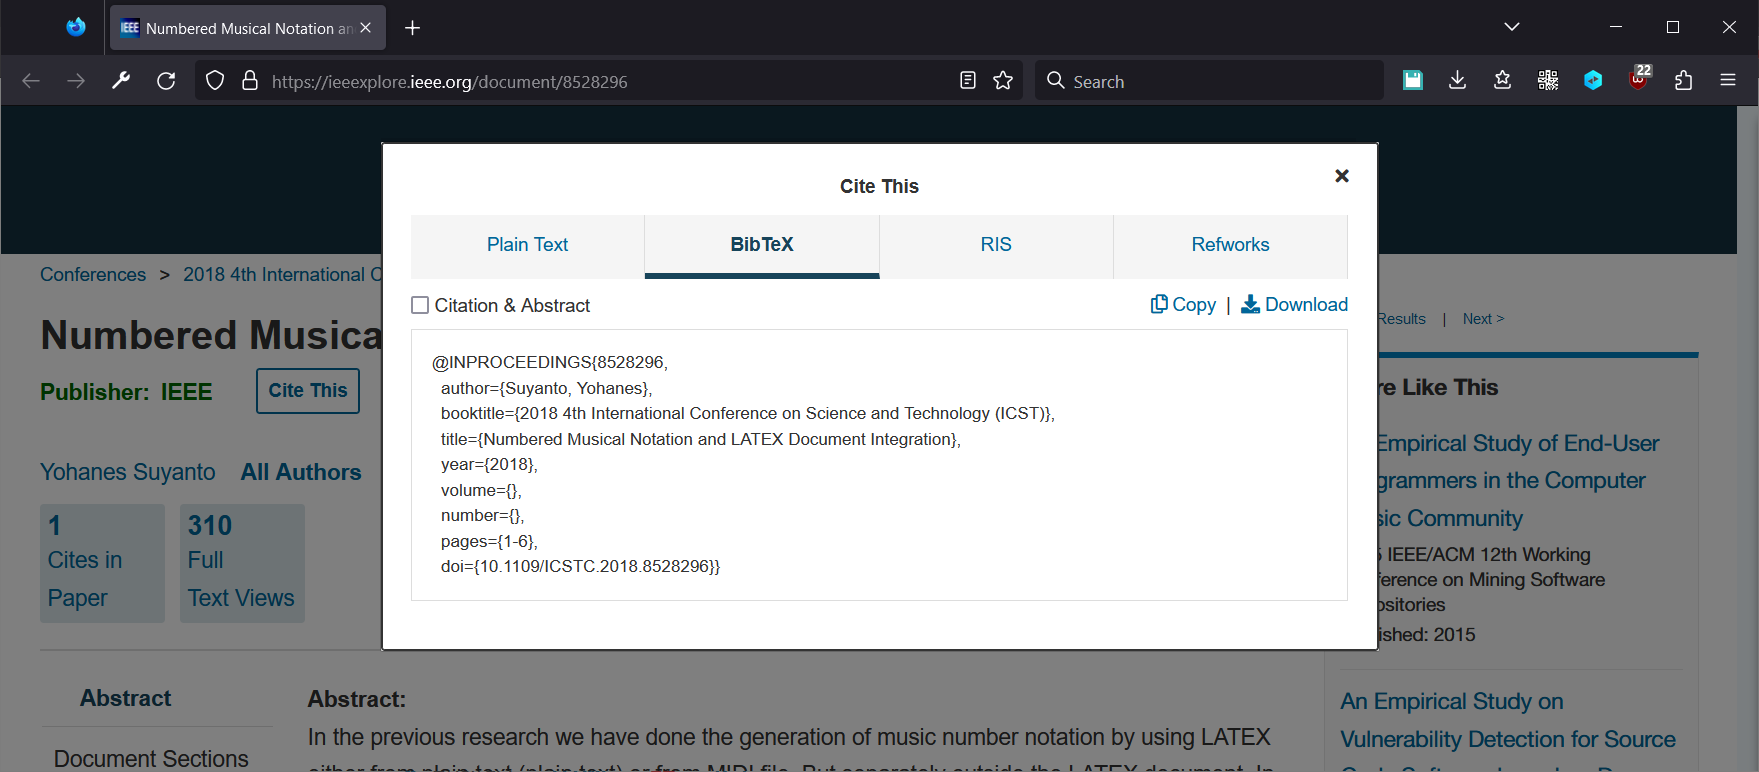
\includegraphics[width=0.75\textwidth]{workbook-extras/ieee-cite-this}
\caption{Запись о литературном источнике в формате BIB на сайте IEEE Xplore}
\label{IEEE Cite This}
\end{figure}
во вкладке "BibTeX" которого можно прочитать и скопировать ссылку на источник в формате BibTeX.

Файл \LaTeX{}, в котором создан настоящий документ, сопровождается текстовым файлом "example-sources.bib", в котором в формате BibTeX приведены все использованные источники.

Для того, чтобы ассоциировать \LaTeX{}-файл со списком источников, в преамбуле файла \LaTeX{} используется директива \verb+\addbibresource+ с именем (путём в файловой системе относительно \LaTeX{}-файла) ассоциируемого BIB-файла, например
\begin{verbatim}
\addbibresource{example-sources.bib}
\end{verbatim}

Можно подключать несколько файлов с источниками литературы, например
\begin{verbatim}
\addbibresource{основные источники.bib}
\addbibresource{мои работы.bib}
\end{verbatim}

Для того, чтобы в тело документа \LaTeX{} вставить непосредственно список литературы, то есть отобразить его в желаемом месте, в этом месте (естественно, внутри окружения \texttt{document} и чаще всего в самом конце) необходимо использовать директиву \verb+\printbibliography+.
Эта директива принимает лишь опциональные параметры, связанные с фильтрацией источников из файла BibTeX, методами отображения источников и~т.~.п.
Однако во многих случаях менять методы отображения не следует, поскольку они уже задаются стандартизированно классом документа \LaTeX{}, который предоставляется организацией, для которой готовится документ.
Поэтому в большинстве случаев достаточно использовать директиву \verb+\printbibliography+ без параметров.

Эта директива выбирает из BibTeX-файла те \textit{и только те} источники, ссылки на которые проставлены в тексте документа рассмотренной выше директивой \verb+\cite+, сортирует их в соответствии с требованиями класса документа или опций, и отображает их в виде списка литературы, опять же в формате, который установлен классом документа и/или опциями.

\paragraph{Формат библиографической записи BibTeX.} Библиографические сведения об источнике литературы начинаются с определения типа источника, который предваряется символом "@" (at).
Распространенными типами являются: книга (\texttt{@book}), раздел книги (\texttt{@inbook}), статья (\texttt{@article}), материалы конференции (\texttt{@conference} или эквивалентный тип \texttt{@inproceedings}), технические мануалы (\texttt{@manual}), диссертации (\texttt{@thesis}), технические спецификации (\texttt{@techreport}), интернет-публикации и веб-сайты (\texttt{@online}) и прочее (\texttt{@misc}).
Существуют и другие типы библиографических источников, с их полным списком можно ознакомится в \cite[разд.~2.1]{biblatex23}.

Далее в фигурных скобках приводятся сведения об источнике.
Во-первых, указывается идентификатор библиографической записи, который используется в ассоциированном документе \LaTeX{} в качестве параметра директивы \verb+\cite+, рассмотренной в разделе~\ref{раздел про cite}.

Во-вторых, через запятую указываются сами сведения о публикации парами "поле=\{значение\}".
Эти сведения включают в себя:
\begin{itemize}
\item авторство, например, \verb+author={Дональд Эрвин Кнут}+;
\item заголовок, например, \verb+title={Все про \TeX{}}+;
\item издательство, например, \verb+publisher={Вильямс}+;
\item адрес издательства (или просто город), например, \verb+address={Москва}+;
\item число страниц, например, \verb+pagetotal={560}+;
\item год издания, например, \verb+year={2003}+;
\item код ISBN, например, \verb+isbn={5-8459-0382-3}+;
\item и другие.
\end{itemize}

Заданная этими примерами библиографическая запись типа \texttt{@book} с идентификатором "TheTexBook" в формате BibTeX будет иметь вид
\begin{verbatim}
@book{TheTexBook,
 title={Все про \TeX{}},
 author={Дональд Эрвин Кнут},
 pagetotal={560},
 isbn={5-8459-0382-3},
 publisher={Вильямс},
 address={Москва},
 year={2003}
}
\end{verbatim}
Результат компиляции и отображения этой записи в списке литературы к настоящему учебному пособию можно наблюдать в записи источника \cite{TheTexBook} (ссылка сформирована командой \verb+\cite{TheTexBook}+).

В зависимости от поля в библиографической записи BibTeX значения могут быть литерального, списочного, буквального, календарного, целочисленного, диапазонного или некоторых других типов.

Значения \textbf{литерального} типа отображается в скомпилированном списке источников так, как они заданы в файле библиографической записи.
Таким является, например, значение заголовка \texttt{title}.

Значения \textbf{списочного} типа перечисляются с разделением элементов с помощью ключевого слова \texttt{and}, а при компиляции документа элементы соответствующего списка группируются процессором расширения \texttt{biblatex} согласно правилам языка и \LaTeX{}-класса документа.
Такими являются значения \texttt{author}, в котором перечисляются авторы источника, \texttt{publisher} и \texttt{address} (а также синоним \texttt{location}), в которых перечисляются соответственно издательства, опубликовавшие источник, и адреса (города) публикации.
Например, авторы могут быть перечислены следующим образом: \texttt{author = \{Петр Иванович Сидоров and Сидор Петрович Иванов and Петров, Иван Сидорович\}}.
В этом примере обратите внимание на последнего автора Ивана Сидоровича Петрова: его имя и отчество указано после фамилии, выделенной запятой --- в отличие от первых двух авторов, которые указаны сначала именем и отчеством и затем --- фамилией.

Отметим, что если элемент значения списочного типа сам по себе должен содержать слово "and", то этот элемент должен обрамляться фигурными скобками.
Так известное издательство Wiley and Sons обрамляется фигурными скобками дважды: \texttt{publisher = \{\{Wiley and Sons\}\}}, поскольку слово "and" является частью названия.

Значения \textbf{буквального} типа подобно значениям литерального типа отображаются при компиляции PDF-файла буквально.
Отличие заключается в том, что в значениях буквального типа разрешается использование специальных символов \LaTeX{}, например, символа "\textbackslash", которые могут требоваться форматами некоторых идентификаторов, таких как DOI (поле \texttt{doi}) или имя файла (поле \texttt{file}).
Предполагается, что в значениях литерального типа необходимость использования таких специальных символов редка настолько, что для их использования можно применять директивы из раздела \ref{раздел про специальные символы} без значительных неудобств для автора файла BIB.
В значениях же буквального типа эти специальные символы могут быть добавлены напрямую.
Кроме этого значения буквального типа могут при компиляции выделяться специальным, в большинстве случаев моноширинным (см. директиву \verb+\texttt+ в табл. \ref{таблица с методами выделения текста}), шрифтом.
Пример использования: \texttt{doi = \{10.1109/ICCSA.2011.47\}}.

Значения \textbf{календарного} типа задают даты в формате "гггг-мм-дд", где "г" --- цифра года, "м" --- месяца, "д" --- дня.
Примерами значений календарного типа являются, во-первых, значение поля \texttt{urldate}, задающее дату доступа к Интернет-ресурсу, например, \texttt{urldate=\{2024-01-20\}}; во-вторых, значение поля \texttt{eventdate}, задающее даты проведения какого-либо события, например, конференции.
Значения календарного типа могут быть диапазонными: через прямой слеш "/" могут указываться дата начала и дата конца события, например, \texttt{eventdate=\{2011-06-20/2011-06-23\}}.
Если даты не заданы или не известны полностью, соответствующий элемент библиографической записи может быть опущен или заменен символами "XX", например, \texttt{eventdate=\{2011-06-XX\}} и \texttt{eventdate=\{2011-06\}}.

Значения \textbf{целочисленного} типа, используются для обозначения томов (поле \texttt{volume}) и порядковых номеров изданий (поле \texttt{edition}).
Такие значения должны быть целыми числами, заданными арабскими или римскими цифрами.
Например, \texttt{volume=\{IV\}} и \texttt{edition=\{2\}}.

\textbf{Диапазонными} значениями задаются целочисленные интервалы, разделяемые одиночным\footnote{Серии дефисов заменяются одним.} дефисом.
При компиляции списка литературы дефисы заменяются знаками диапазона (описанными в разделе \ref{раздел про дефис}).
Применяются такие значения, например, при указании страниц в сборнике публикаций: \texttt{pages=\{123-134\}}.

Обратите внимание на то, что в таких часто используемых полях, как \texttt{number} (номер журнала), \texttt{part} (часть литературной работы), \texttt{pagetotal} (число страниц), \texttt{month} (месяц публикации), \texttt{year} (год публикации), номера \texttt{isbn} и \texttt{issn}, используются значения литерального типа.

Полный список типов значений и их соответствие различным полям приведен в \cite[раздел~2]{biblatex23}.

В зависимости от типа библиографического источника те или иные сведения могут быть обязательными, опциональными или не нужными (игнорируемыми).
Доступные для создания библиографических BibTeX-записей некоторых (распространенных и перечисленных выше) типов обязательные и опциональные поля представлены в таблице~\ref{таблица с полями BibTeX}.

Назначение большинства полей очевидно из их названия, вместе с тем читатель может самостоятельно ознакомиться с подробностями в \cite[раздел~2]{biblatex23}.

\pagebreak
\small
\begin{longtable}{|l|p{0.25\textwidth}|p{0.44\textwidth}|}
\caption{Поля некоторых типов библиографических записей формата BibTeX}
\label{таблица с полями BibTeX}
\endfirsthead
\caption{Поля некоторых типов библиографических записей формата BibTeX \itshape(продолжение)}
\endhead
\hline
\thead{Тип BibTeX} & \thead{Обязательные\\поля} & \thead{Опциональные поля} \\
\hline
\texttt{@article}
 & \texttt{author, title, journaltitle, year/date}
 & \texttt{translator, annotator, commentator, subtitle, titleaddon, editor, editora, editorb, editorc, journalsubtitle, journaltitleaddon, issuetitle, issuesubtitle, issuetitleaddon, language, origlanguage, series, volume, number, eid, issue, month, pages, version, note, issn, addendum, pubstate, doi, eprint, eprintclass, eprinttype, url, urldate}\\
\hline
\texttt{@book}
 & \texttt{author, title, year/date}
 & \texttt{editor, editora, editorb, editorc, translator, annotator, commentator, introduction, foreword, afterword, subtitle, titleaddon, maintitle, mainsubtitle, maintitleaddon, language, origlanguage, volume, part, edition, volumes, series, number, note, publisher, location, isbn, eid, chapter, pages, pagetotal, addendum, pubstate, doi, eprint, eprintclass, eprinttype, url, urldate}\\
\hline
\texttt{@inbook}
 & \texttt{author, title, booktitle, year/date}
 & \texttt{bookauthor, editor, editora, editorb, editorc, translator, annotator, commentator, introduction, foreword, afterword, subtitle, titleaddon, maintitle, mainsubtitle, maintitleaddon, booksubtitle, booktitleaddon, language, origlanguage, volume, part, edition, volumes, series, number, note, publisher, location, isbn, eid, chapter, pages, addendum, pubstate, doi, eprint, eprintclass, eprinttype, url, urldate}\\
\hline
\texttt{@manual}
 & \texttt{author/editor, title, year/date}
 & \texttt{subtitle, titleaddon, language, edition, type, series, number, version, note, organization, publisher, location, isbn, eid, chapter, pages, pagetotal, addendum, pubstate, doi, eprint, eprintclass, eprinttype, url, urldate}\\
\hline
\texttt{@misc}
 & \texttt{author/editor, title, year/date}
 & \texttt{subtitle, titleaddon, language, howpublished, type, version, note, organization, location, month, addendum, pubstate, doi, eprint, eprintclass, eprinttype, url, urldate}\\
\hline
\texttt{@online}
 & \texttt{author/editor, title, year/date, doi/eprint/url}
 & \texttt{subtitle, titleaddon, language, version, note, organization, month, addendum, pubstate, eprintclass, eprinttype, urldate}\\
\hline
\makecell{\texttt{@inproceedings}\\и \texttt{@conference}}
 & \texttt{author, title, booktitle, year/date}
 & \texttt{editor, subtitle, titleaddon, maintitle, mainsubtitle, maintitleaddon, booksubtitle, booktitleaddon, eventtitle, eventtitleaddon, eventdate, venue, language, volume, part, volumes, series, number, note, organization, publisher, location, month, isbn, eid, chapter, pages, addendum, pubstate, doi, eprint, eprintclass, eprinttype, url, urldate}\\
\hline
\texttt{@techreport}
 & \texttt{author, title, type, institution, year/date}
 & \texttt{subtitle, titleaddon, language, number, version, note, location, month, isrn, eid, chapter, pages, pagetotal, addendum, pubstate, doi, eprint, eprintclass, eprinttype, url, urldate}\\
\hline
\texttt{@thesis}
 & \texttt{author, title, type, institution, year/date}
 & \texttt{subtitle, titleaddon, language, note, location, month, isbn, eid, chapter, pages, pagetotal, addendum, pubstate, doi, eprint, eprintclass, eprinttype, url, urldate}
\\
\hline
\end{longtable}
\normalsize

Пример библиографической записи о материале конференции:
\begin{verbatim}
@inproceedings{Kaneko,
 author={Kaneko, Masataka and Takato, Setsuo},
 booktitle={2011 International Conference on
  Computational Science and Its Applications},
 title={A CAS Macro Package as LaTeX Graphical Command
  Generator and Its Applications},
 pages={72-81},
 doi={10.1109/ICCSA.2011.47},
 eventdate={2011-06-20/2011-06-23},
 url={https://ieeexplore.ieee.org/document/5959564},
 urldate={2023-12}
}
\end{verbatim}

Пример библиографической записи о научной статье:
\begin{verbatim}
@article{фармацевты,
 author = {Frank, Thomas and Gastine, Silke and Lindauer,
  Klaus and Speth, Heiner and Strougo, Ashley
  and Kovar, Andreas},
 title = {LaTeX tutorial for the standardization and
  automation of population analysis reports},
 journal = {CPT: Pharmacometrics \& Systems Pharmacology},
 volume = {10},
 number = {11},
 pages = {1310-1322},
 keywords = {guidelines, LaTeX, pharmacodynamics, population
  pharmacokinetics, report, template},
 doi = {https://doi.org/10.1002/psp4.12705},
 year = {2021},
 publisher={{John Wiley and Sons, Inc.}}
}
\end{verbatim}

\section*{Заключение}
В настоящем документе достаточно поверхностно описаны основные аспекты использования языка \LaTeX{} и его расширений для подготовки документации.

Назначение данного документа --- ознакомить читателя с \LaTeX{} в мере, достаточной для реализации только основных задач при подготовки документации.
Поэтому данный материал ни в коей мере не претендует на полноту, а читателю рекомендуется ознакомиться по мере возможности и возникающих требований со ссылками, которые указаны в тексте документа и приведены в списке литературы ниже.

Вместе с тем, для реализации собственных задач достаточно часто можно просто модифицировать существующие \LaTeX{} файлы, например тот, на основе которого собран данный документ, подменяя существующее содержание и параметры директив своими.

Документ в большой степени ориентирован на написание технической документации, содержащей формулы, алгоритмы, таблицы и рисунки, однако может быть применен и для решения более широкого круга задач.

Кроме собственно \LaTeX{} в настоящем документе приведено описание класса \texttt{fefudoc}, который используется для подготовки документов в ДВФУ.
Основным назначением данного класса является автоматизация основных аспектов оформления таких документов, поэтому он по большей части лишь устанавливает необходимые параметры отображения документа, а набор собственных директив мал и ограничен теми, которые представлены в разделах \ref{раздел про структуру документа} и \ref{раздел про выделение текста}.

В современных реалиях использование более развитых альтернатив по сравнению с несколько устаревающими проприетарными программами, такими как WYSIWYG-редакторы вроде Microsoft Word, видится перспективным и более удобным.

%\clearpage
\printbibliography

\end{document}

